\chapter{Hardware Development}

This chapter covers the development of 3 separate modular sensor payloads, designed in line with our team's concept of operations of modular autonomy. These 3 payloads, Mk. 0, Mk. 1, and Drone, were carried by 3 modular robots, R1, R2, and D1 respectively during the Tunnel Circuit event. A picture of each robot with its payload can be seen in Figure \ref{glamour_shots}. The individual payloads can be seen in Figure \ref{payloads}. A summary of the components and capabilities of each payload is given in Section \ref{Summary of Payloads}. Each payload is capable of performing all of the high level perception and planning tasks for the robot that carries it, and performs all computation on board.

The Mk. 0 payload was the first sensor payload to be built, and is inspired by the use of the "Blue Payload", a payload similar to the Kaarta Traak \cite{kaarta_traak} which is capable of state estimation. Mk. 0 proved to be too heavy to carry on D1 and was thus simplified into the Drone payload. Mk. 0 also has certain hardware limitations and proved to be difficult to maintain, both of which were addressed during the design of Mk. 1. These two payloads maintain the same mounting mechanism and similar form factors, allowing for interchangeability between R1 and R2. A component level schematic for Mk. 1, the most capable payload of the 3, is given in Figure \ref{mk_1_architecture}.

\begin{figure}
	\centering
	\begin{subfigure}{0.32\textwidth}
		\includegraphics[width=\textwidth]{glamour_shots/r1.jpg}
		\caption{R1 with Mk. 0 Payload}
		\label{r1_glamour}
	\end{subfigure}		
	\hfill
	\begin{subfigure}{0.32\textwidth}
		\includegraphics[width=\textwidth]{glamour_shots/r2.jpg}
		\caption{R2 with Mk. 1 Payload}
		\label{r2_glamour}		
	\end{subfigure}
	\hfill
	\begin{subfigure}{0.32\textwidth}
		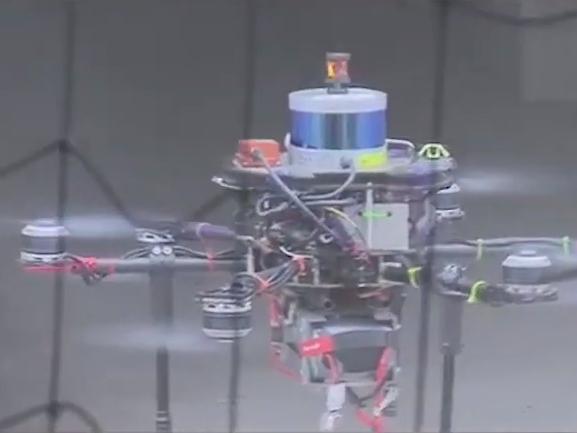
\includegraphics[width=\textwidth]{glamour_shots/d1.png}
		\caption{D1 with Drone Payload}
		\label{d1_glamour}
	\end{subfigure}	
	\caption{Tunnel Circuit robots with sensing payloads}
	\label{glamour_shots}
\end{figure}

\begin{figure}
	\centering
	\begin{subfigure}{0.32\textwidth}
		\includegraphics[width=\textwidth]{mk0_close.jpg}
		\caption{Mk. 0 Payload Close-up}
		\label{mk0_close}
	\end{subfigure}		
	\hfill
	\begin{subfigure}{0.32\textwidth}
		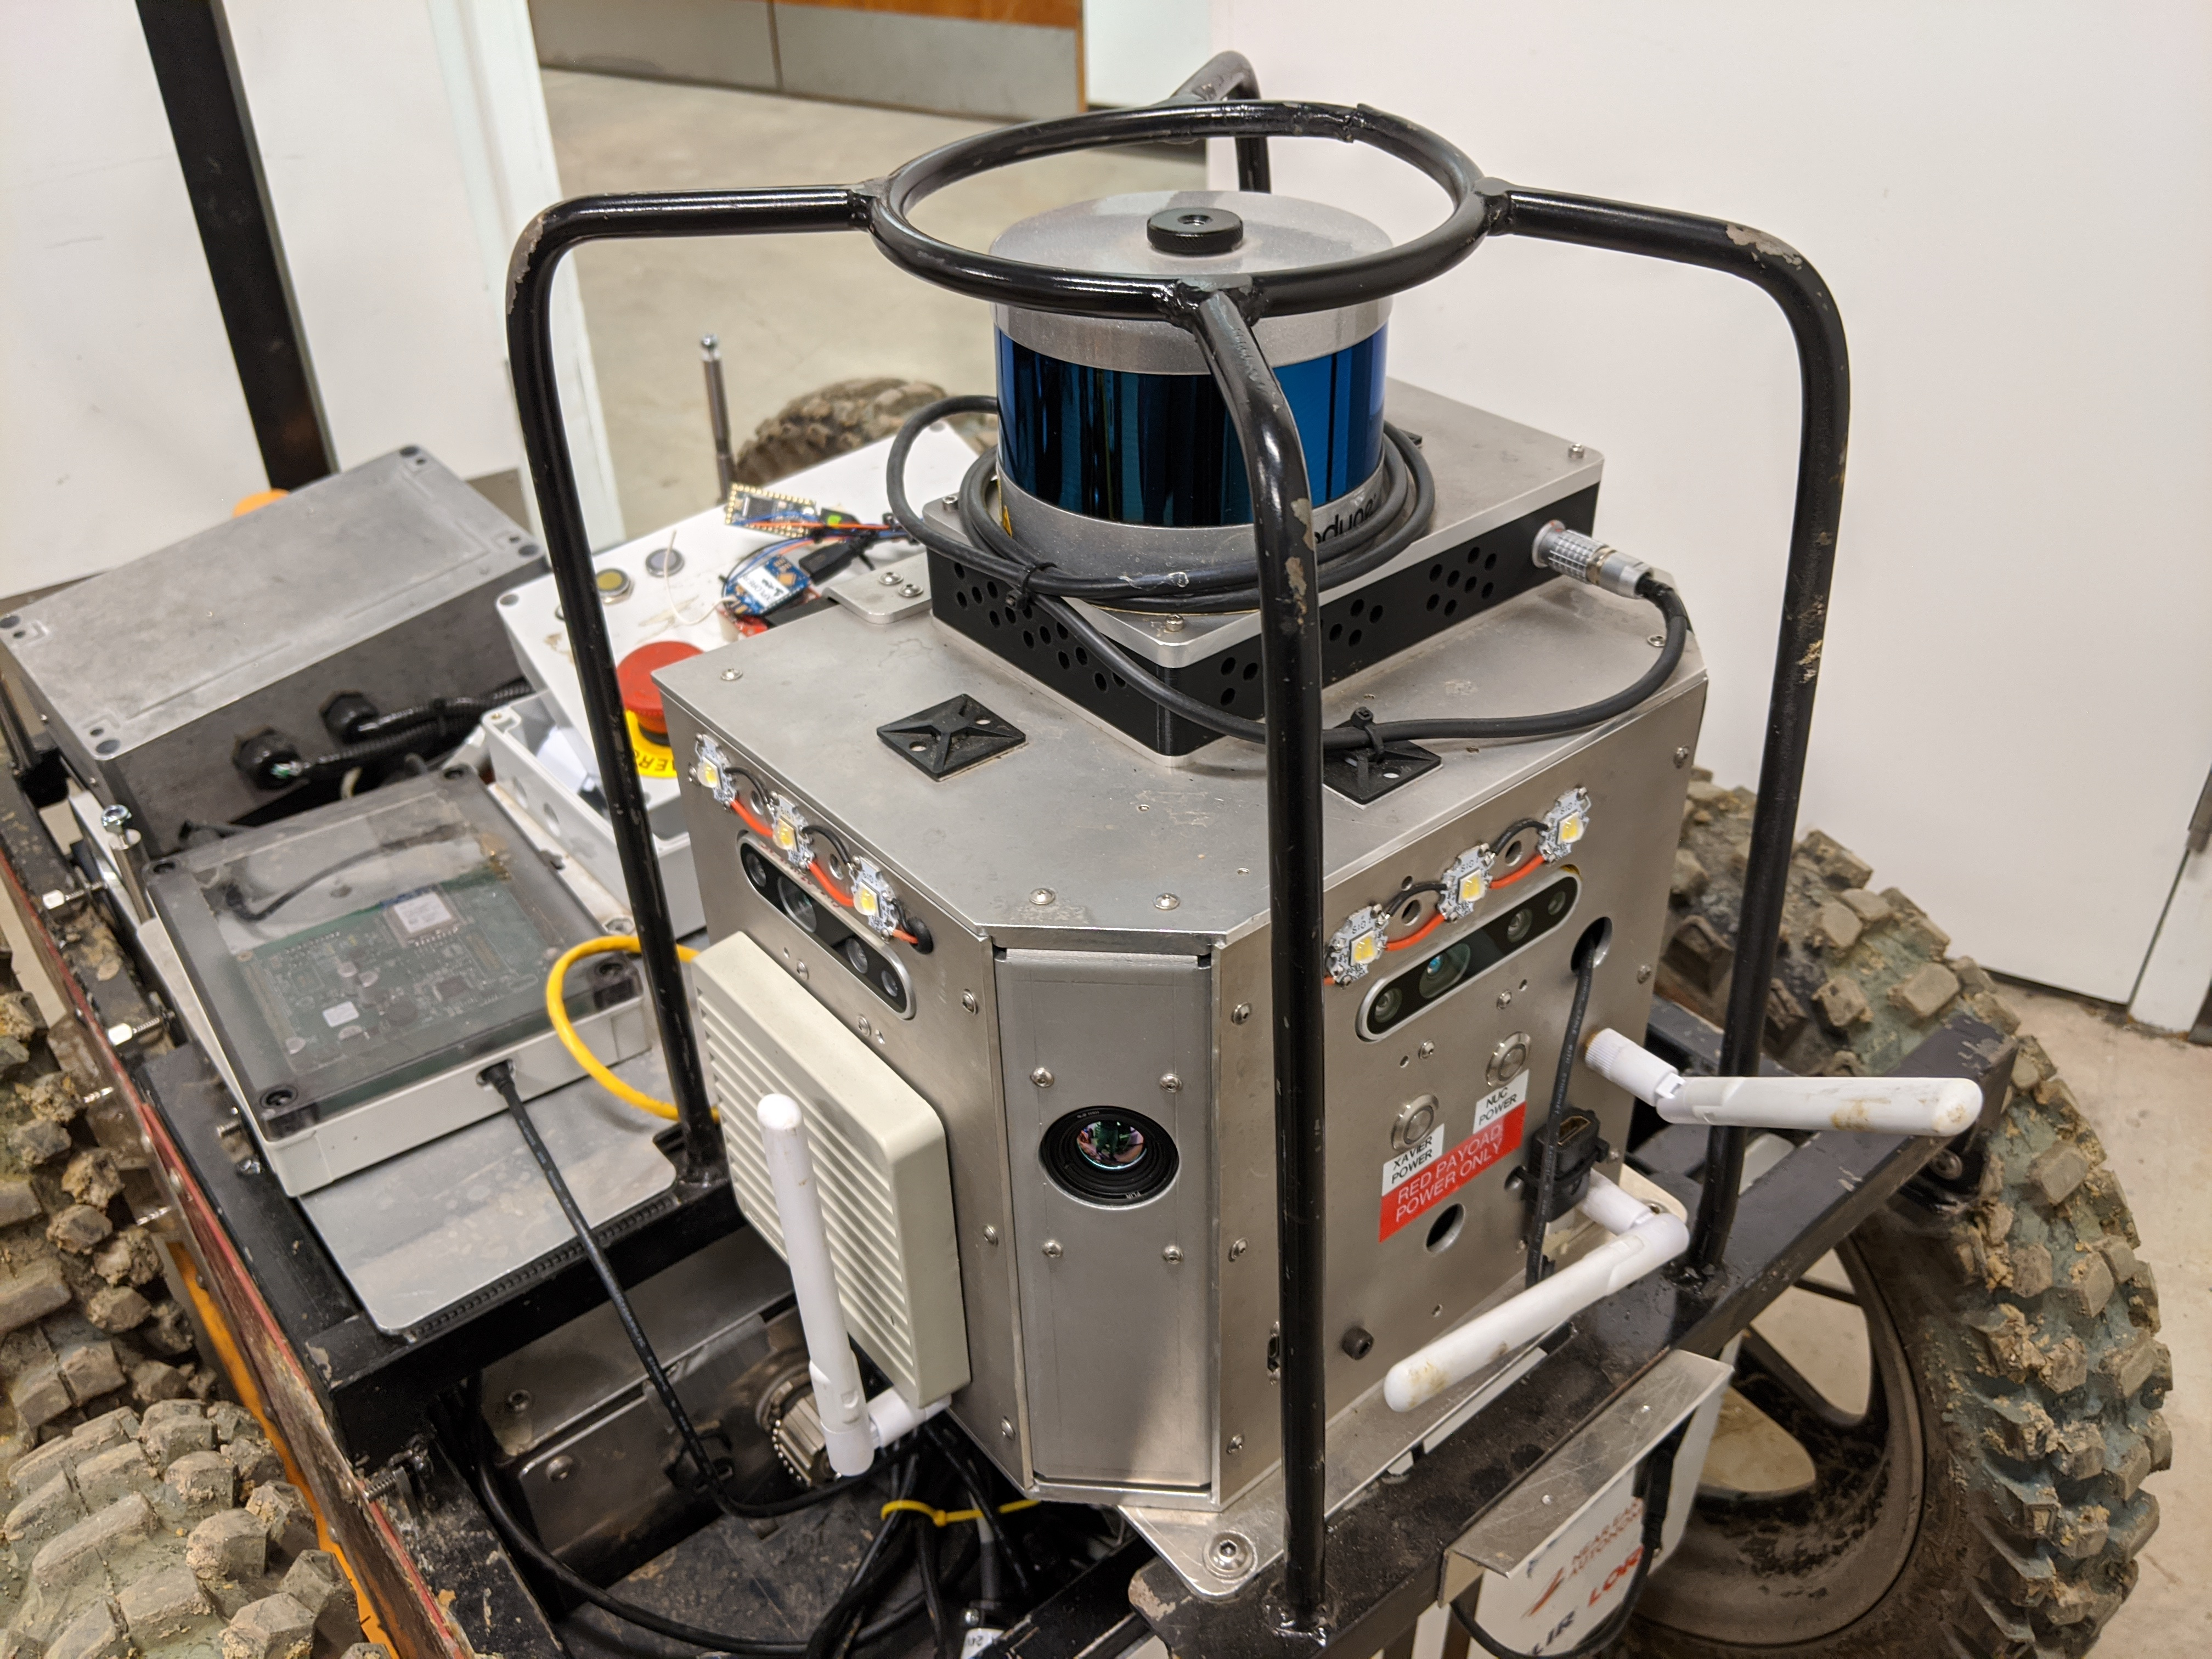
\includegraphics[width=\textwidth]{mk1_close.jpg}
		\caption{Mk. 1 Payload Close-up}
		\label{mk1_close}		
	\end{subfigure}
	\hfill
	\begin{subfigure}{0.32\textwidth}
		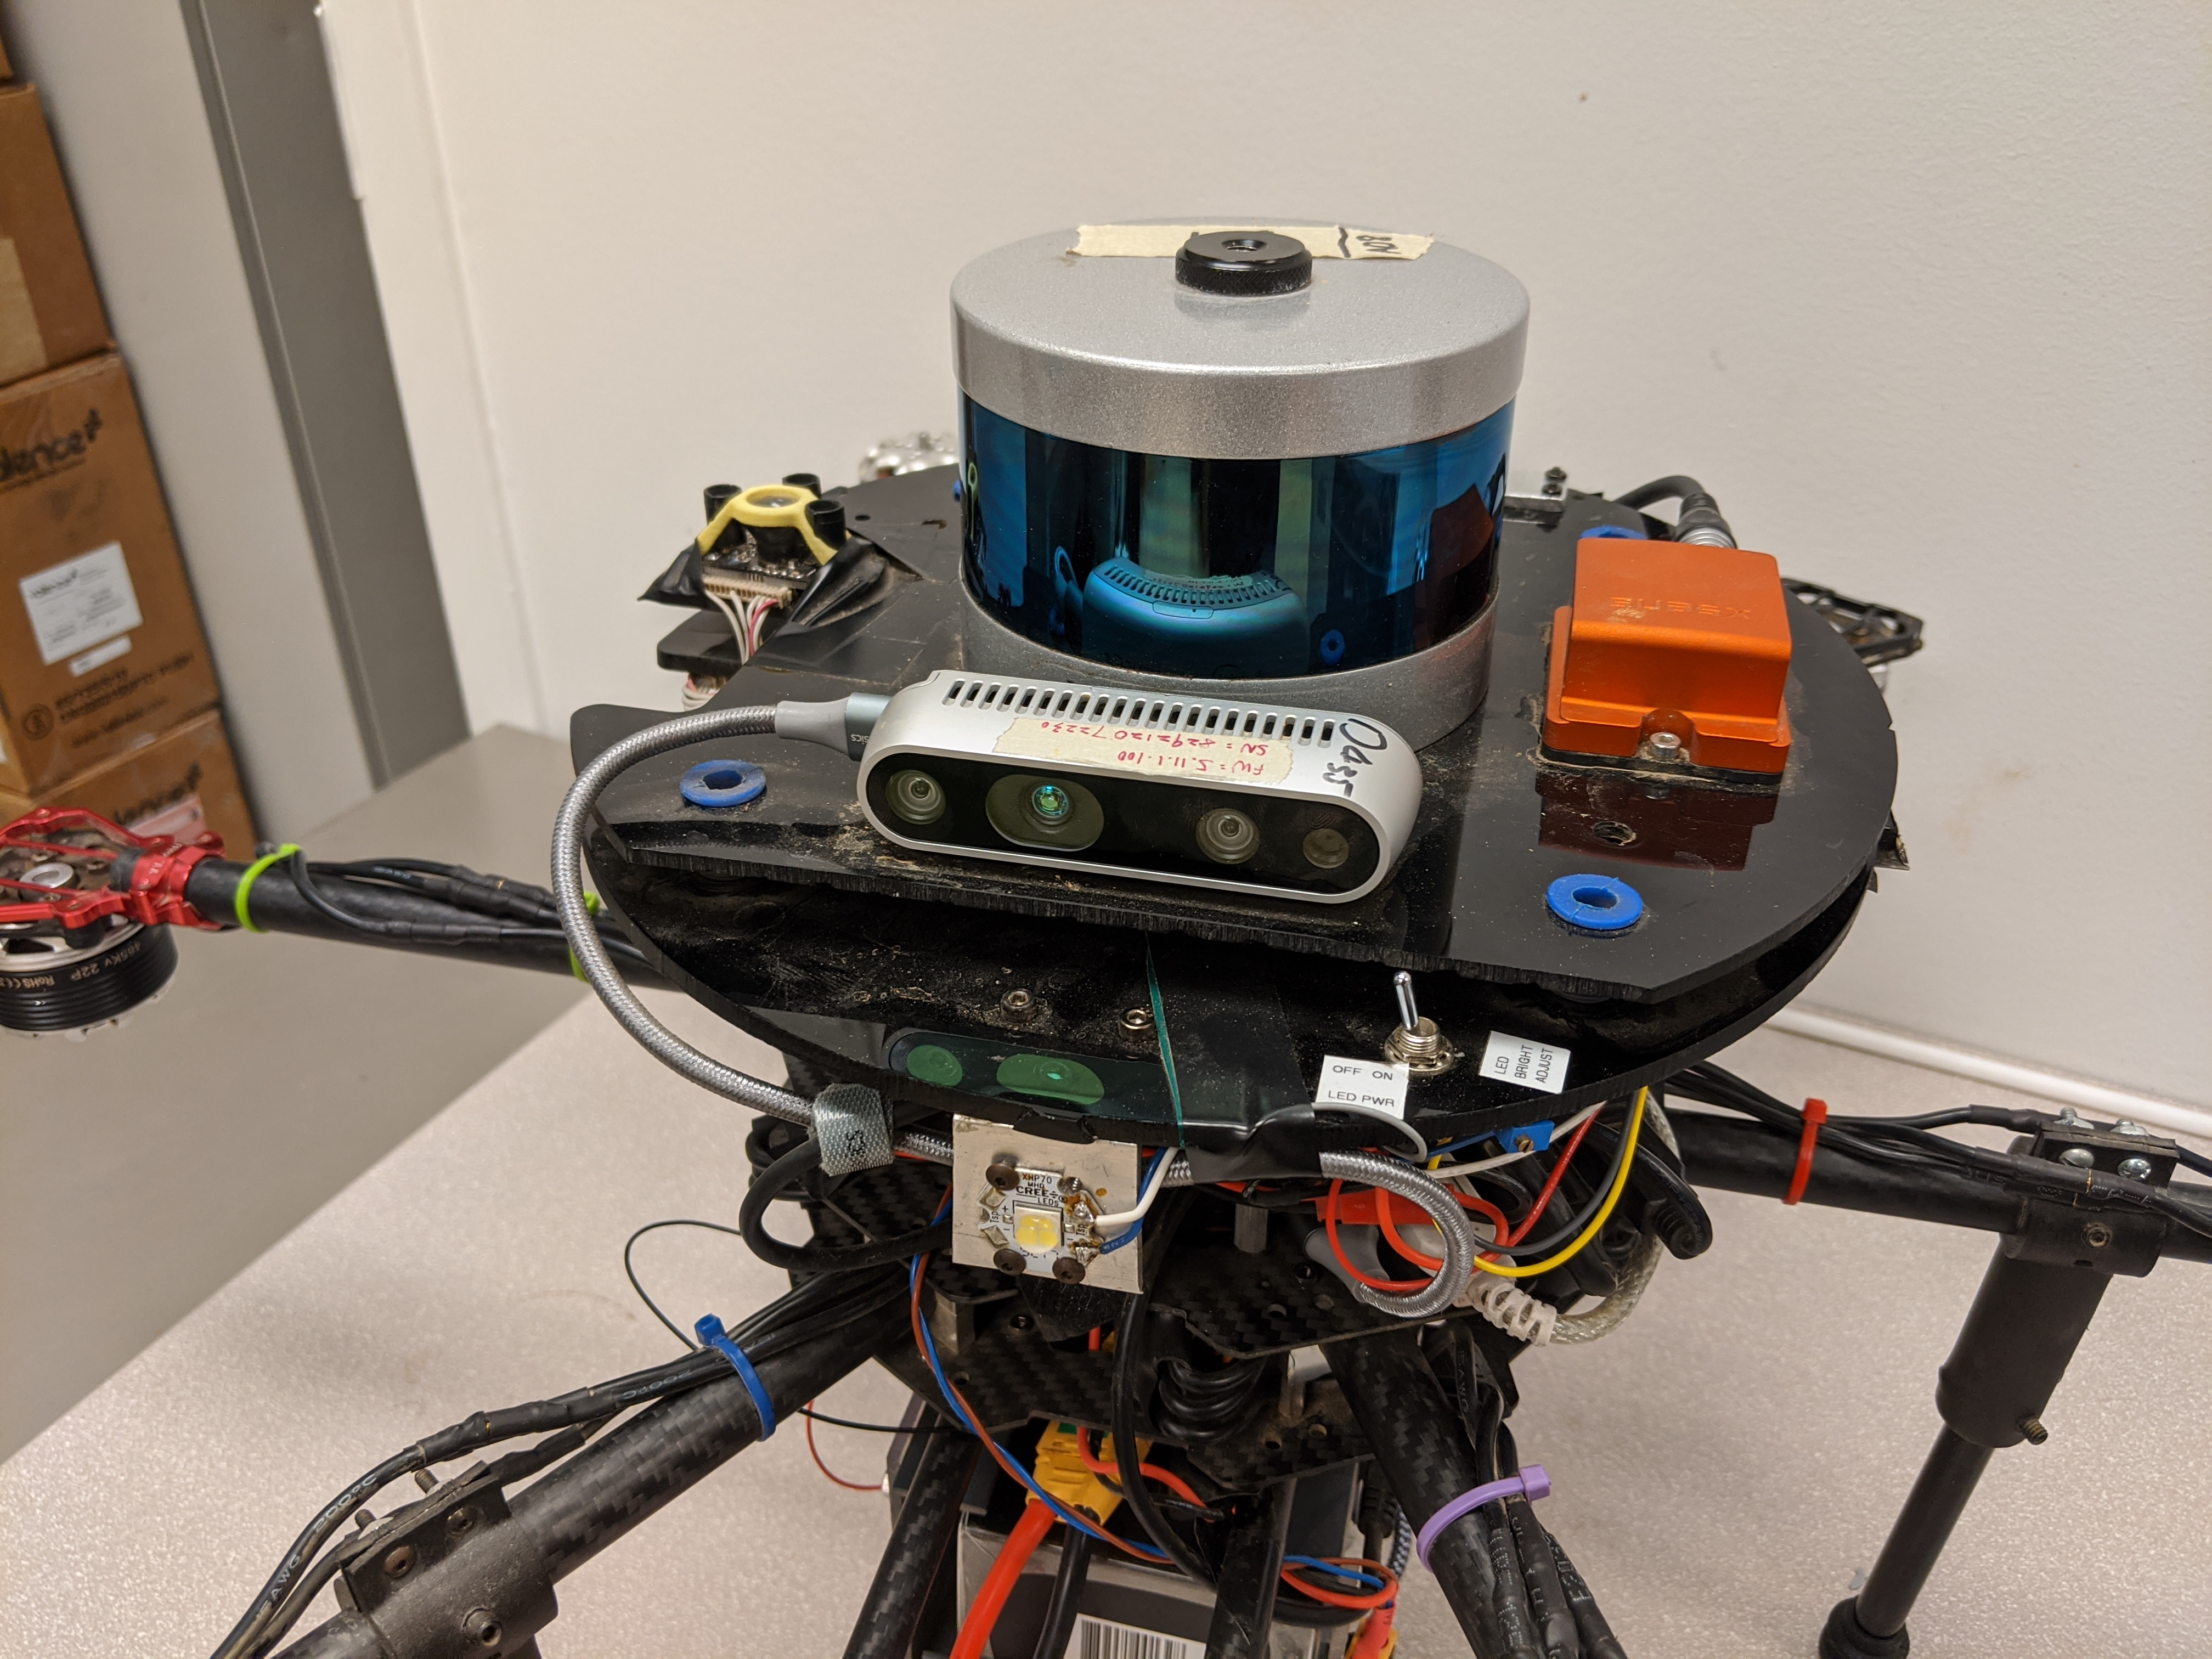
\includegraphics[width=\textwidth]{d1_close.jpg}
		\caption{Drone Payload Close-up}
		\label{drone_closeup}
	\end{subfigure}	
	\caption{Tunnel Circuit payload close-ups}
	\label{payloads}
\end{figure}


\begin{figure}
	\centering
	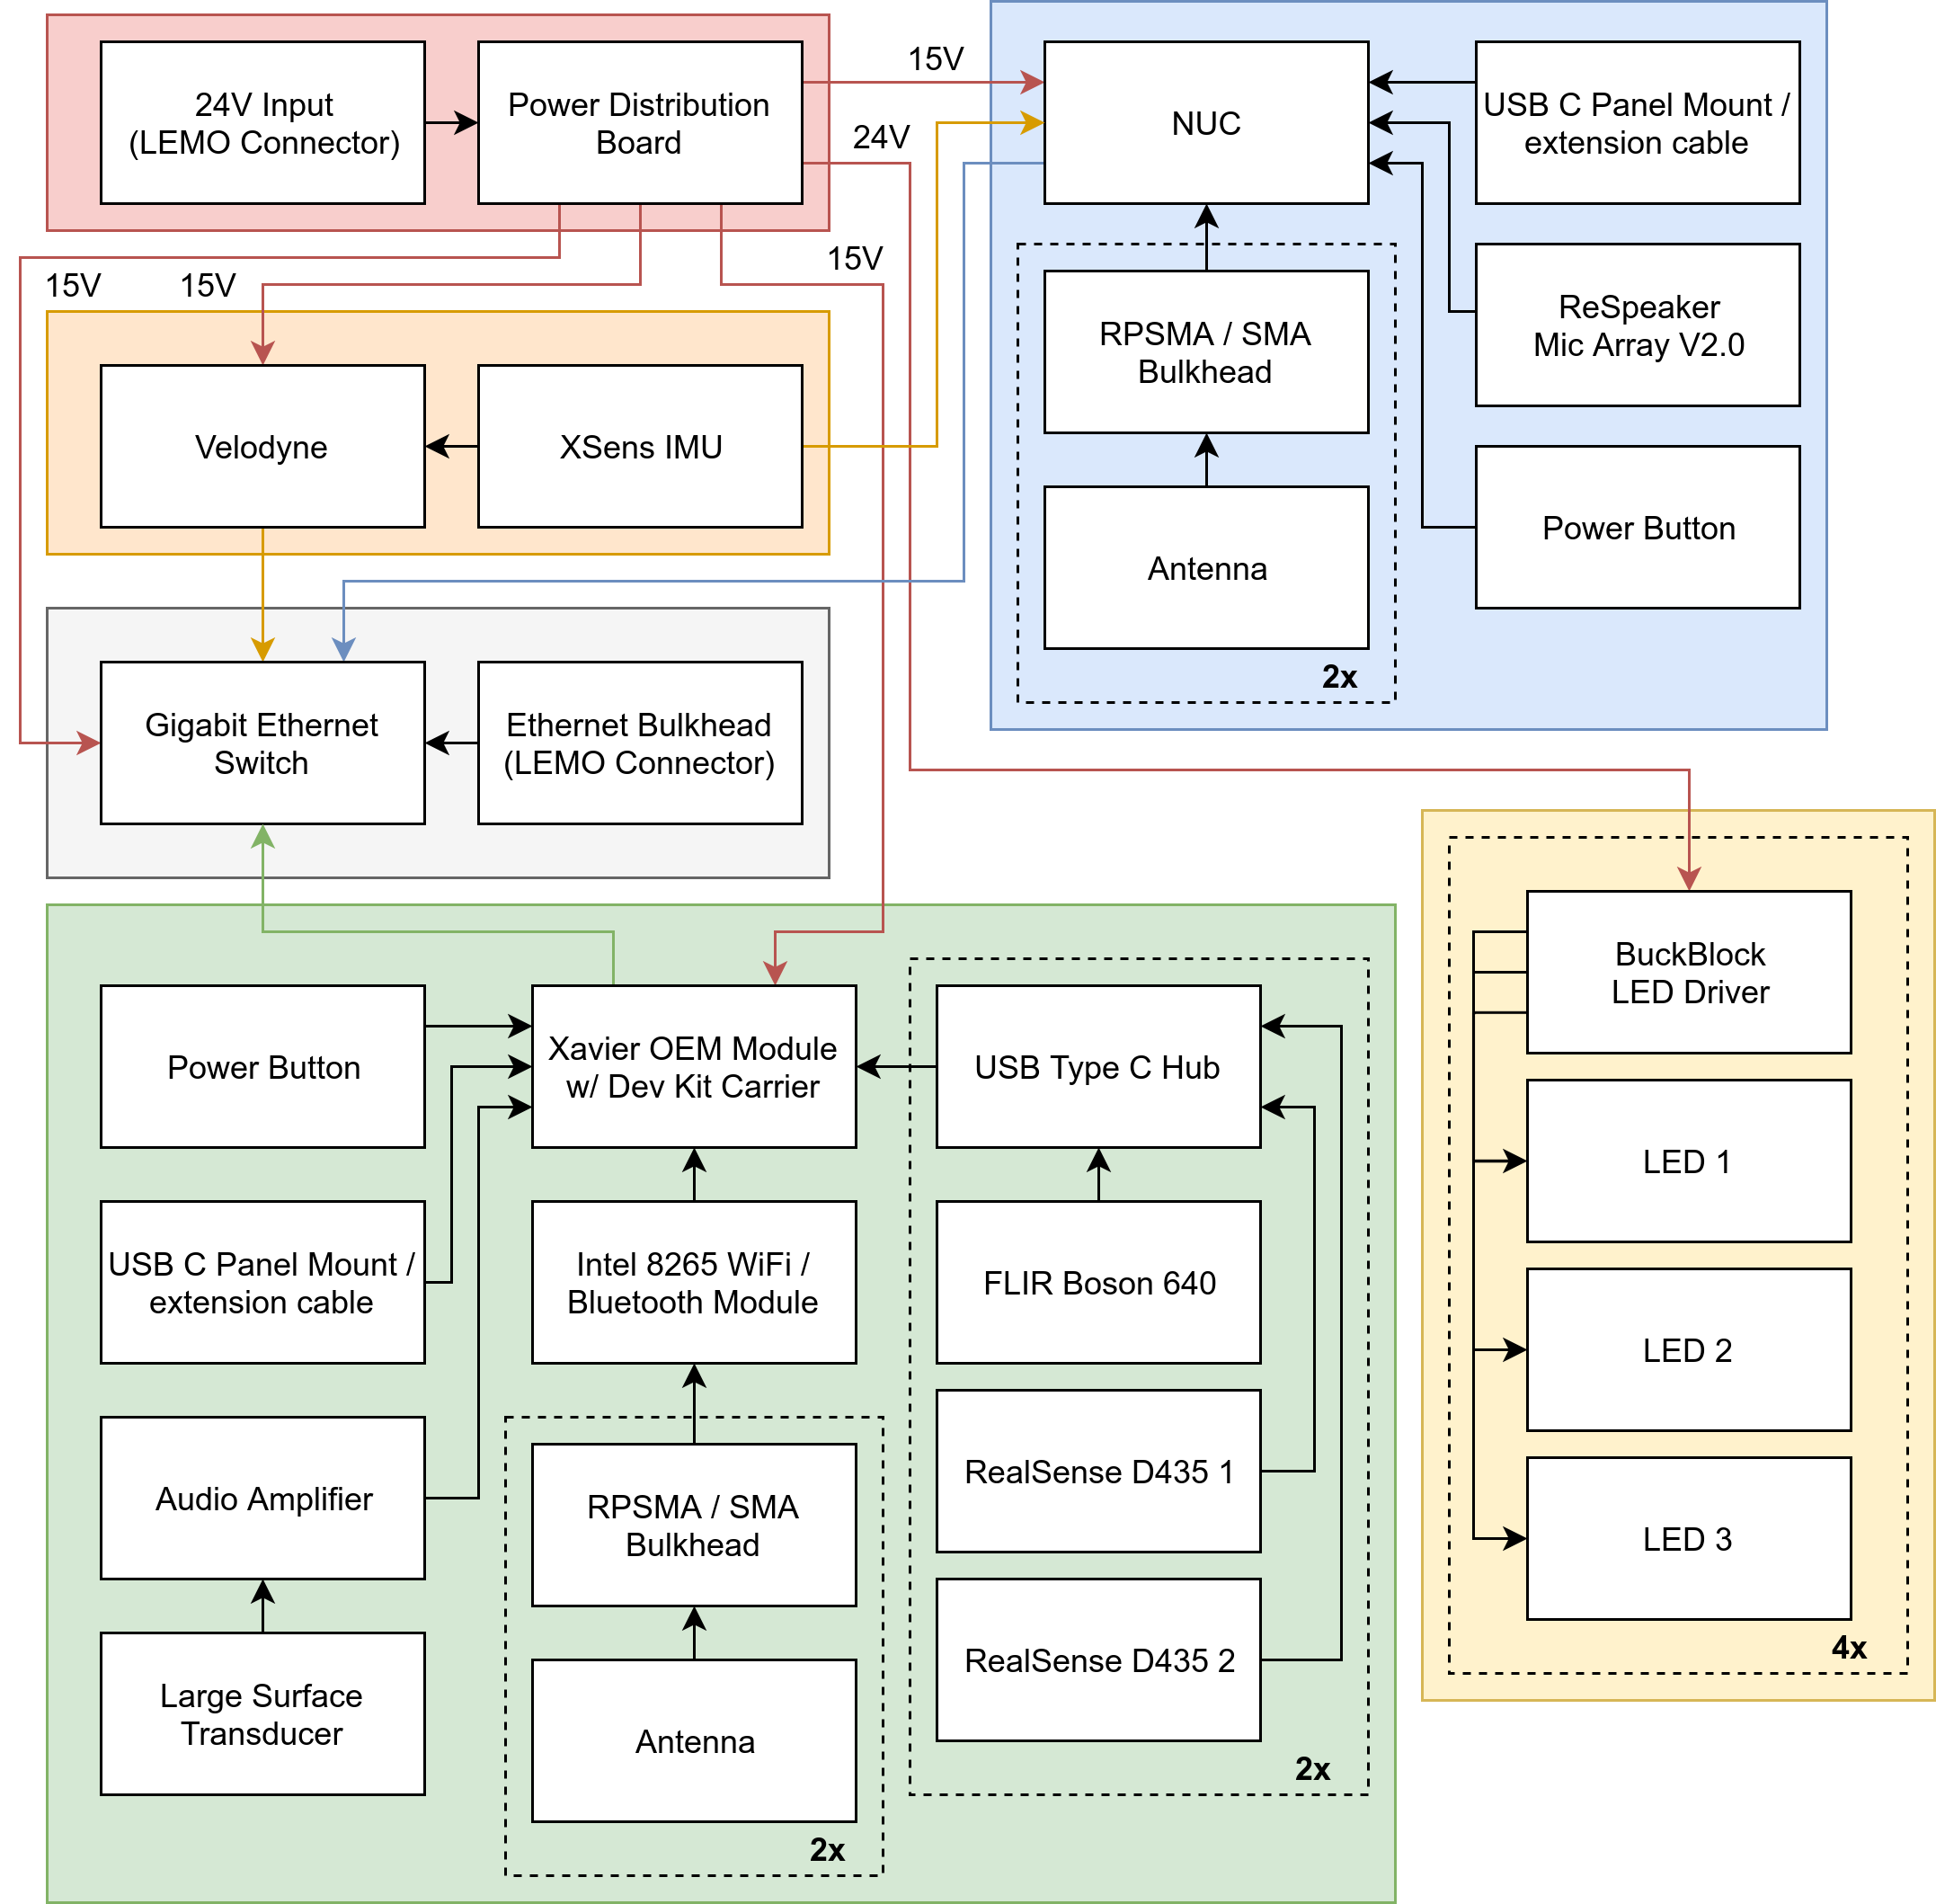
\includegraphics[width=\textwidth]{mk_1_architecture.png}
	\caption[Subsystem diagram for Mk. 1 payload]{Subsystem diagram for the Mk. 1 payload showing the major electrical components present. Payload case fans are not depicted. All state estimation and planning computation happens on the NUC. The Xavier is dedicated solely to artifact detection and localization.}
	\label{mk_1_architecture}
\end{figure}

\section{Payload Requirements}

Inspiration for the design and feasibility of a modular sensing payload resulted from using the Blue payload, a prototype state estimation payload similar to the Kaarta Traak \cite{kaarta_traak}. The payload is self-contained, and can easily be transferred between small and large ground and air robots, as shown in Figure \ref{blue payload robots}. It is simple to use and integrate, requiring only power and a network connection to provide state estimation output. Though the Blue payload's sensing and compute capabilities are insufficient for the complete planning and perception challenges of the DARPA Subterranean Challenges, its use served as the basis for the following hardware requirements (HWR) set for Mk. 0, the first payload built. The requirements are also derived from the timeline and obstacles imposed by the SubT Challenge.

\begin{figure}
	\centering
	\begin{subfigure}{0.32\textwidth}
		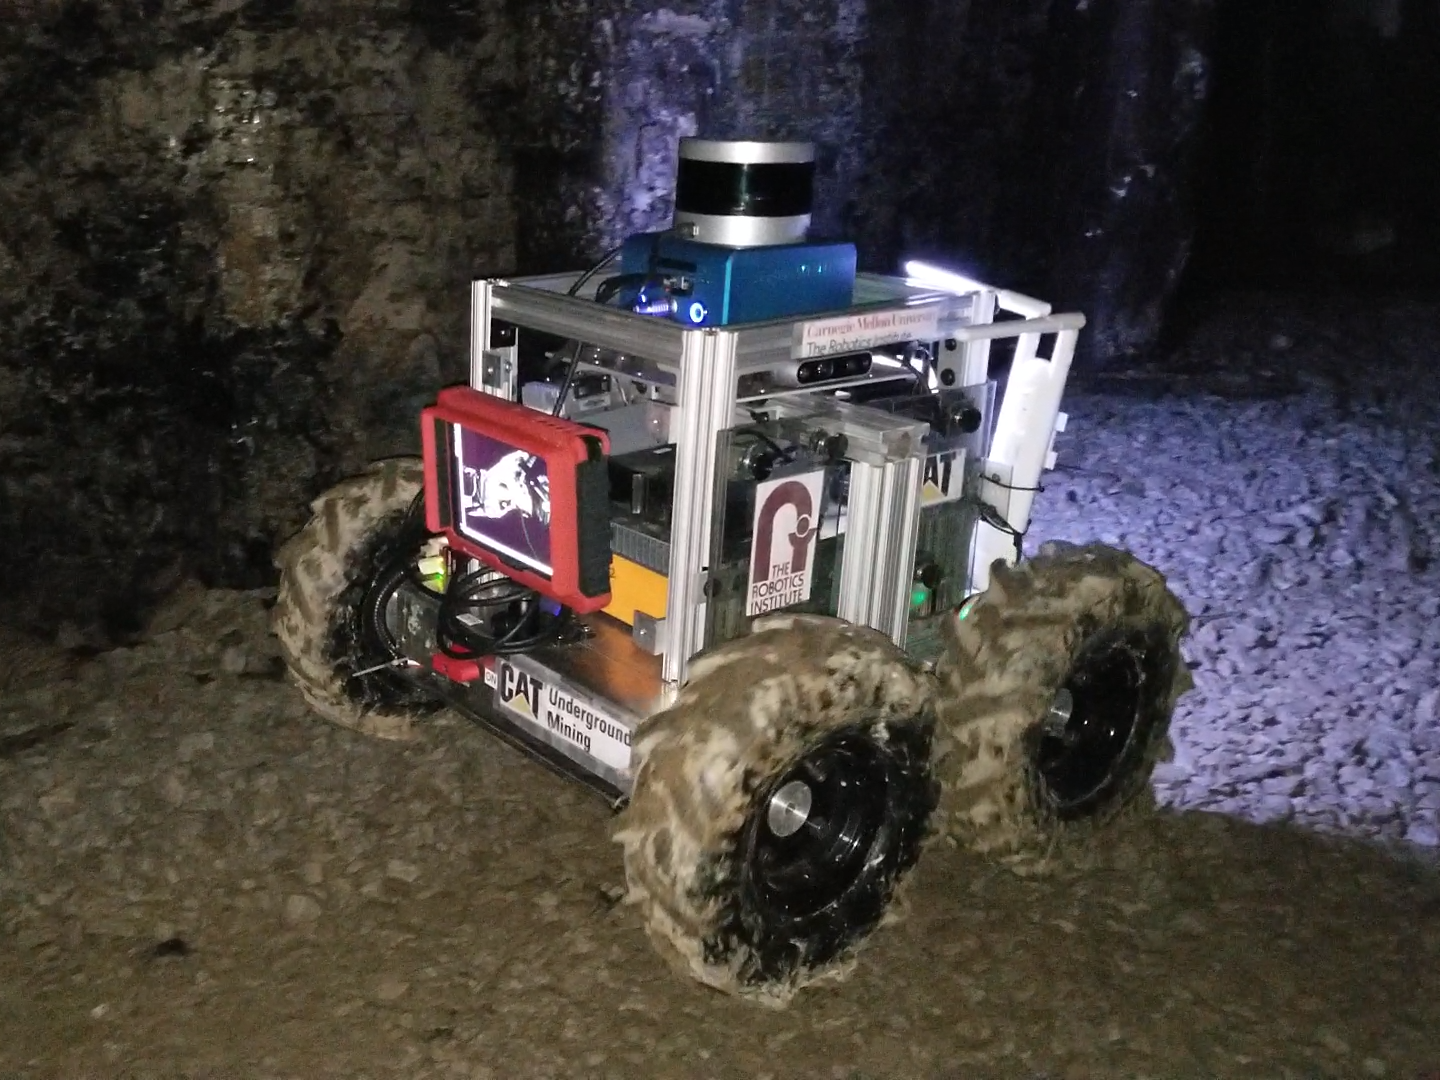
\includegraphics[width=\textwidth]{blue_payload/blue_payload_joeybot_cropped.png}
		\caption{Joeybot with Blue Payload}
		\label{joeybot blue payload}
	\end{subfigure}		
	\hfill
	\begin{subfigure}{0.32\textwidth}
		\includegraphics[width=\textwidth]{blue_payload/r1_with_blue_payload.jpg}
		\caption{R1 with Blue Payload}
		\label{r1 blue payload}		
	\end{subfigure}
	\hfill
	\begin{subfigure}{0.32\textwidth}
		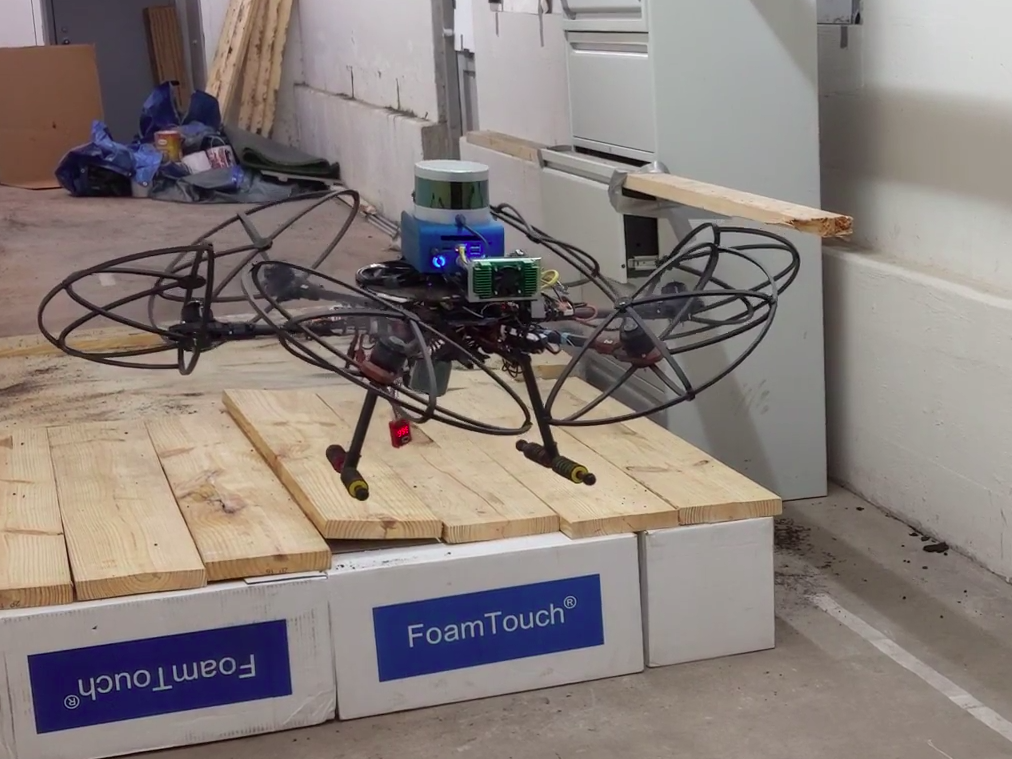
\includegraphics[width=\textwidth]{blue_payload/drone_with_blue_payload_cropped.png}
		\caption{D1 with Blue Payload}
		\label{d1 blue payload}
	\end{subfigure}	
	\caption[Early robots carrying the Blue payload]{The picture shows 3 robots of different sizes each carrying the same Blue payload. Joeybot is a small test platform developed for early testing of autonomy code, but was not used during the Tunnel Circuit. The depicted aerial vehicle is a prototype of D1, featuring tilted rotors instead of level ones.}
	\label{blue payload robots}
\end{figure}

\begin{description}
	\item[HWR1: Rapid Development] There were a little under 3 months from the beginning of the competition (September 2018) to the first qualification deadline (December 2018), by which time the payload must be completed. This short timeline heavily incentivizes drawing from previous experience and familiarity, such as with components and sensors, and prefers in-house manufacturing capabilities with short lead times.
	\item[HWR2: Self-contained] All of the sensing and computation for the high level autonomy features should happen inside the payload itself. Ideally, the payload would only be supplied power and a network connection, just like the Blue Payload, and would output autonomy goals (such as waypoints) and information (such as robot state, maps, and artifact locations) to be relayed to the human supervisor at the base station.
	\item[HWR3: Environmental Robustness] The field environments for the SubT competition events were expected to be somewhat hostile to the sensors. Specifically, the rules mention that "dust, fog, mist, water, and smoke are within scope" for the Tunnel Circuit \cite{tunnel_rules}, and thus the payload should be reasonably protected against these elements. The payload should also be robust to the mechanical loading it would be subject to as a result of rough terrain.
	\item[HWR4: Weight Sensitivity] The Blue payload demonstrated that the ability to use the same payload between ground and aerial platforms, as in Figure \ref{blue payload robots}, was useful in building modular systems, and the same ability was desired for the Mk. 0 payload. The relatively low payload capacity of D1 set a hard upper bound on the weight of Mk. 0, though as low of a weight as possible was preferred due to the inverse relationship between weight and flight time.	
	\item[HWR5: Cost Sensitivity] Though there aren't specific cost restrictions imposed for the robots or payloads, DARPA is interested in identifying cost effective solutions for the SubT Challenge. Minimizing cost is also useful as a design goal to support the creation of multiple copies or iterations of Mk. 0, rather than just a single expensive prototype.
\end{description}

\section{Mk. 0 Component Selection}

The first step in the development of Mk. 0 was the selection of the individual sensors, computers, and supporting components which would be packaged inside the payload. HWR2 (rapid development) dictated that, where possible, familiar components were selected to reduce the time necessary to develop the payload. This was the primary consideration in certain cases, such as with the LIDAR selection. Other components, such as the RGB cameras, were compared against other candidates which significantly exceeded the familiar choice in some metric, such as HWR4 (weight sensitivity), HWR5 (cost sensitivity), or data quality. The unfamiliar choice was chosen if its increased performance or satisfaction of requirements outweighed the decreased familiarity.

It is important to note the context for the development of Mk. 0. During its design, the preliminary planning and navigation stack was being developed and tested on Joeybot, carrying the Blue payload. Work on the artifact detection and localization software pipeline had barely begun. The early stages of these software components meant that sensor processing capabilities and compute requirements were unknown, necessitating educated guesses. Where multiple choices were available, components were selected to allow for the most flexibility in future software algorithms, even at the cost of lower priority requirements.

\subsection{Computer Selection}

Each sensor payload performs 3 broad tasks -- state estimation, path planning and navigation, and artifact detection and localization. Though specific resource requirements weren't known at this stage, previous experience and available literature could be used to make approximations. Computer selection was considered for each task separately.

\subsubsection{State Estimation}

The state estimation system used on the Blue payload is LOAM \cite{zhang2014loam}, the current state of the art for SLAM as measured on the KITTI dataset \cite{Geiger2013IJRR}. Its performance, as well as the familiarity developed with it while working on Joeybot with the Blue payload, made it an easy selection for the SLAM system for all payloads. LOAM was specifically tuned to run on the hardware inside the Blue payload, which has an Intel NUC with an Intel Core i7 processor inside. To avoid the potentially time consuming process of tuning LOAM to run on a different hardware platform, the NUC was selected as a required component for Mk. 0. Specifically, the NUC8i7BEH model was used as it was the NUC board with the most powerful CPU available at the time. LOAM utilizes the majority of 2 cores, leaving an additional 2 physical cores potentially open for other tasks.

\subsubsection{Path Planning and Navigation}

The path planning and navigation stack was being actively developed on Joeybot and ran on Joeybot's internal computer, a mid-range industrial-grade PC from Logic Supply. Though the Logic Supply computer was also using an Intel Core i7 processor, the processor itself was underclocked to reduce heat output. Profiling indicated that it should be possible to run the path planning and navigation stack on the 2 available cores of the NUC being used to run LOAM. Significant increases in the compute load were not expected, so it was decided to use a single NUC8i7BEH to run both LOAM and the path planning and navigation stack to avoid increasing system complexity.

\subsubsection{Artifact Detection and Localization}

At this stage, work on the artifact detection and localization pipeline had just begun. It was unclear what the final approach would be, and thus predicting its computational requirements proved difficult. Convolutional neural networks were shown in the literature to outperform traditional methods in a number of machine perception benchmarks \cite{deng2009imagenet,Geiger2013IJRR,lin2014microsoft}, and were thus expected to be a part of the pipeline. However, they require a significant amount of computing resources to run at high framerates (10+ Hz). Multiple neural networks would potentially need to be run in parallel, depending on the quantity of image-based sensors selected. The following hardware platforms were considered, each selected for being small enough and robust enough for inclusion in a modular sensing payload. 

\begin{enumerate}
	\item Intel Movidius Neural Compute Stick
	\item Integrated GPU on selected NUC (Intel Iris Plus Graphics 655)
	\item Nvidia Jetson TX2
	\item Nvidia Jetson AGX Xavier
\end{enumerate}

Of the available options, the Nvidia Jetson AGX Xavier ("Xavier") offers the highest inference performance due to its many CUDA cores, as well as its specialized Tensor Cores and Deep Learning Accelerators (DLA). Combined, the Xavier is capable of performing more than an order of magnitude more FLOPS (floating point operations per second) than the other platforms, but has the highest cost of all options and weighs the most by a small margin. As no specific compute requirements were determined for the artifact detection and localization stack at this time, the Xavier was selected to provide the highest ceiling for available compute resources.

\subsubsection{LOAM on Xavier}

The option of using the Xavier to run the entire autonomy stack, consisting of state estimation, path planning and navigation, and artifact detection and localization, was briefly considered but summarily dismissed due to a belief that the Xavier's CPU would be insufficient. After the completion of the Mk. 0 payload, some experiments were performed to determine the validity of this hypothesis. Profiling of the NUC revealed that LOAM was one of the heaviest processes, consuming nearly 100\% of a single core in some circumstances, and smaller portions of other cores. Thus, porting LOAM to the Xavier was the first test.

Before benchmarking LOAM on the Xavier, all CPU and GPU cores on the Xavier were enabled (MAX-N mode), and had their frequency maximized. The frequency governor was disabled, and the fan on the Xavier Developer Kit was permanently set to run at the maximum speed to prevent overheating during tests. After setup, LOAM was run in a few different configurations on the Xavier on a playback of pre-recorded data. For each configuration, a downsampling parameter was adjusted which controlled the number of points kept from the laser scan point clouds during a preprocessing step before scan matching inside LOAM. A lower number of points used during scan matching typically results in a lower match accuracy, but requires fewer cpu cycles to run. Additional scans received during scan matching are dropped, requiring that scan matching complete under the output rate of clouds from the LIDAR (10 Hz), and resulting in higher scan matching error otherwise. Figure \ref{loam_xavier} shows a visualization of the results.

\begin{figure}
	\centering
	\begin{subfigure}{0.32\textwidth}
		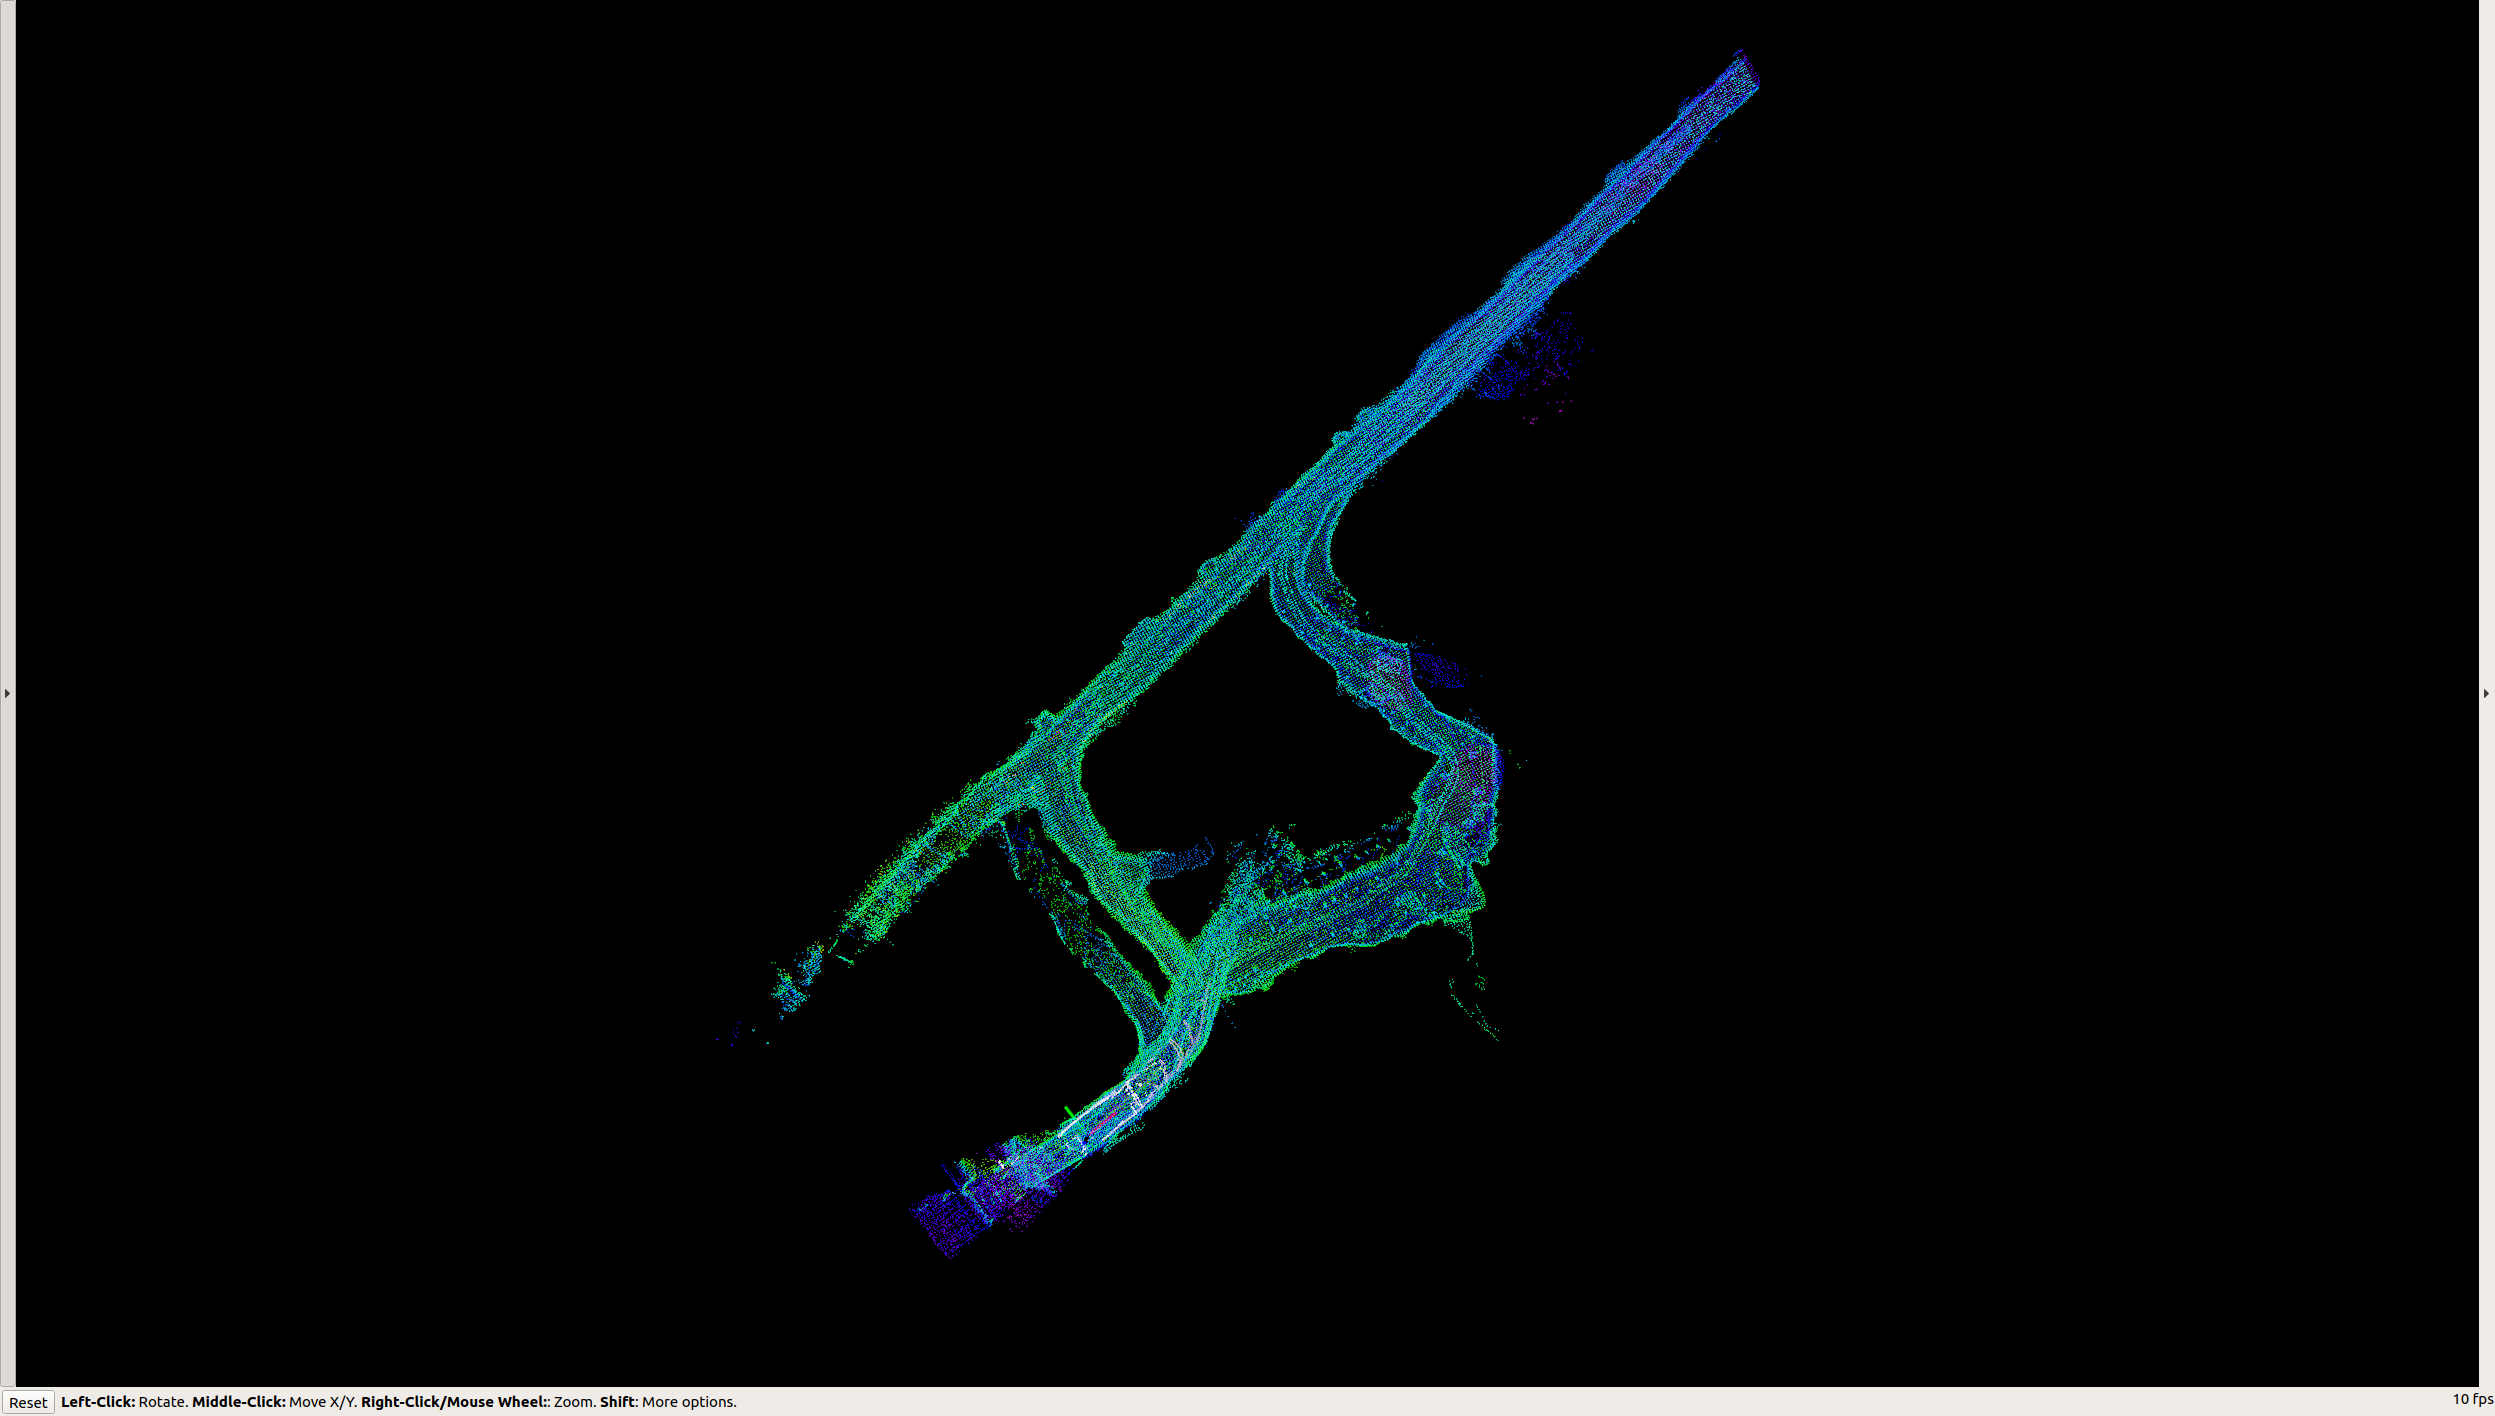
\includegraphics[width=\textwidth]{tour_ed_mine_1-00.png}
		\caption{100\% points kept}
		\label{loam_xavier_100}
	\end{subfigure}		
	\hfill
	\begin{subfigure}{0.32\textwidth}
		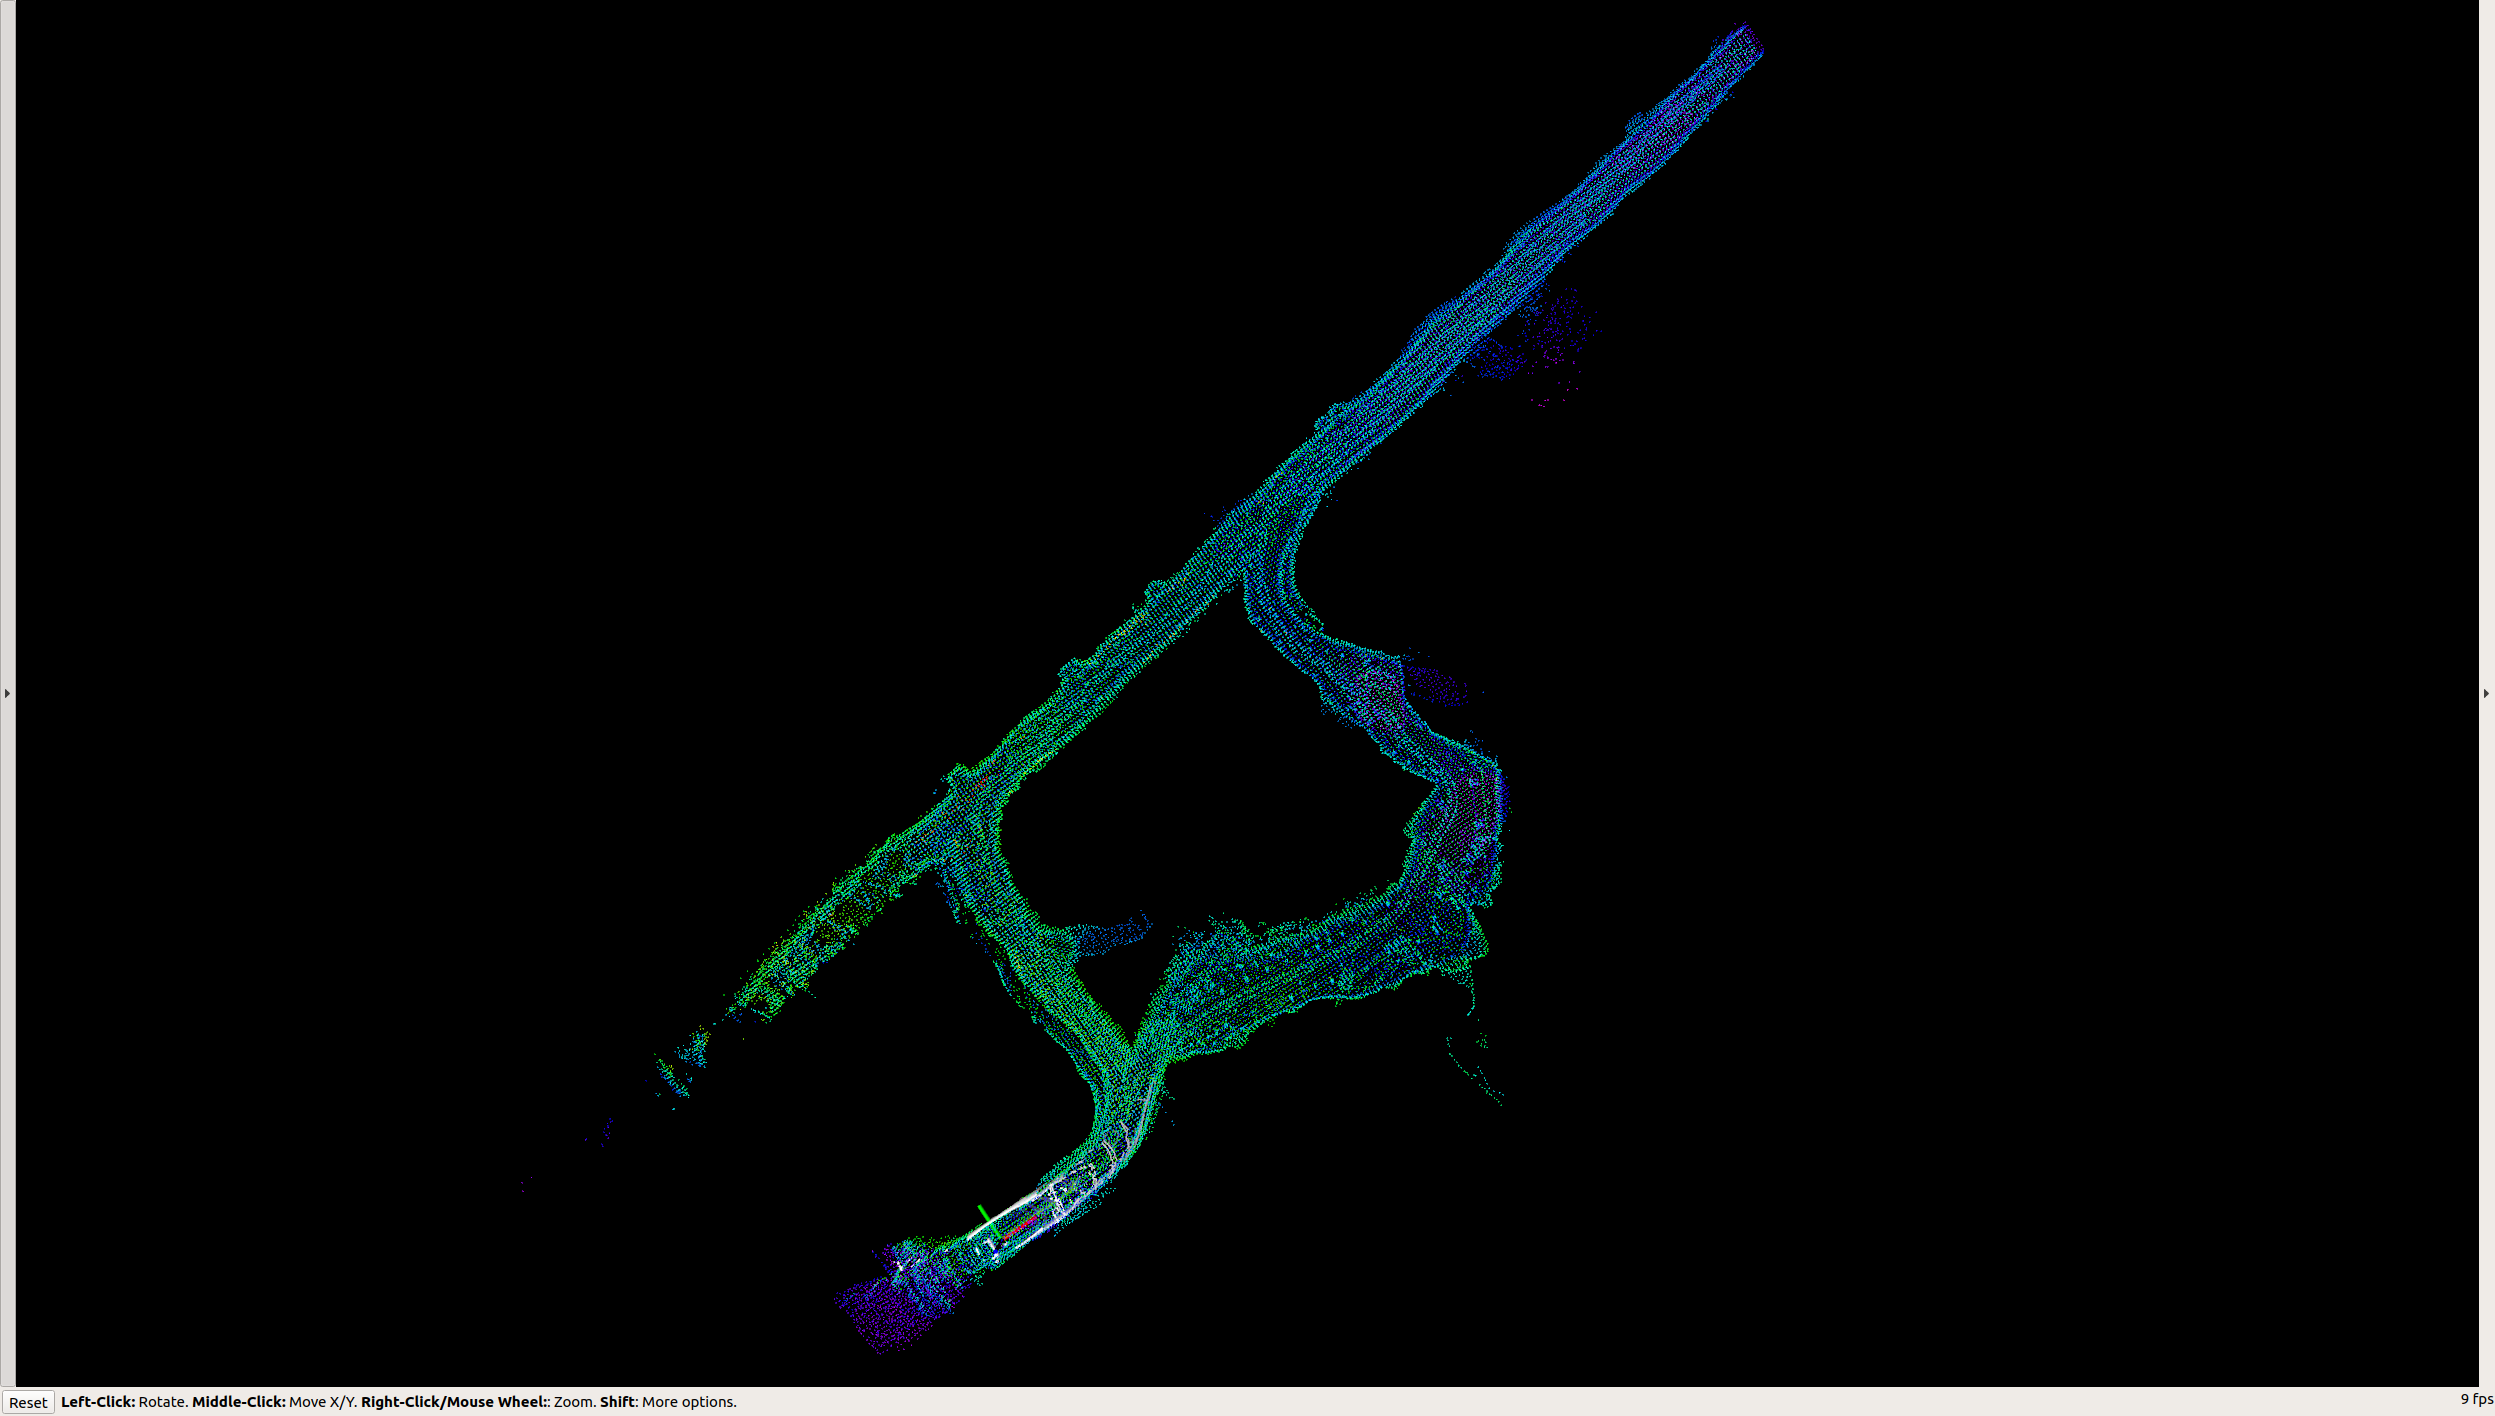
\includegraphics[width=\textwidth]{tour_ed_mine_1-00_1-25s.png}
		\caption{75\% points kept}
		\label{loam_xavier_75}		
	\end{subfigure}
	\hfill
	\begin{subfigure}{0.32\textwidth}
		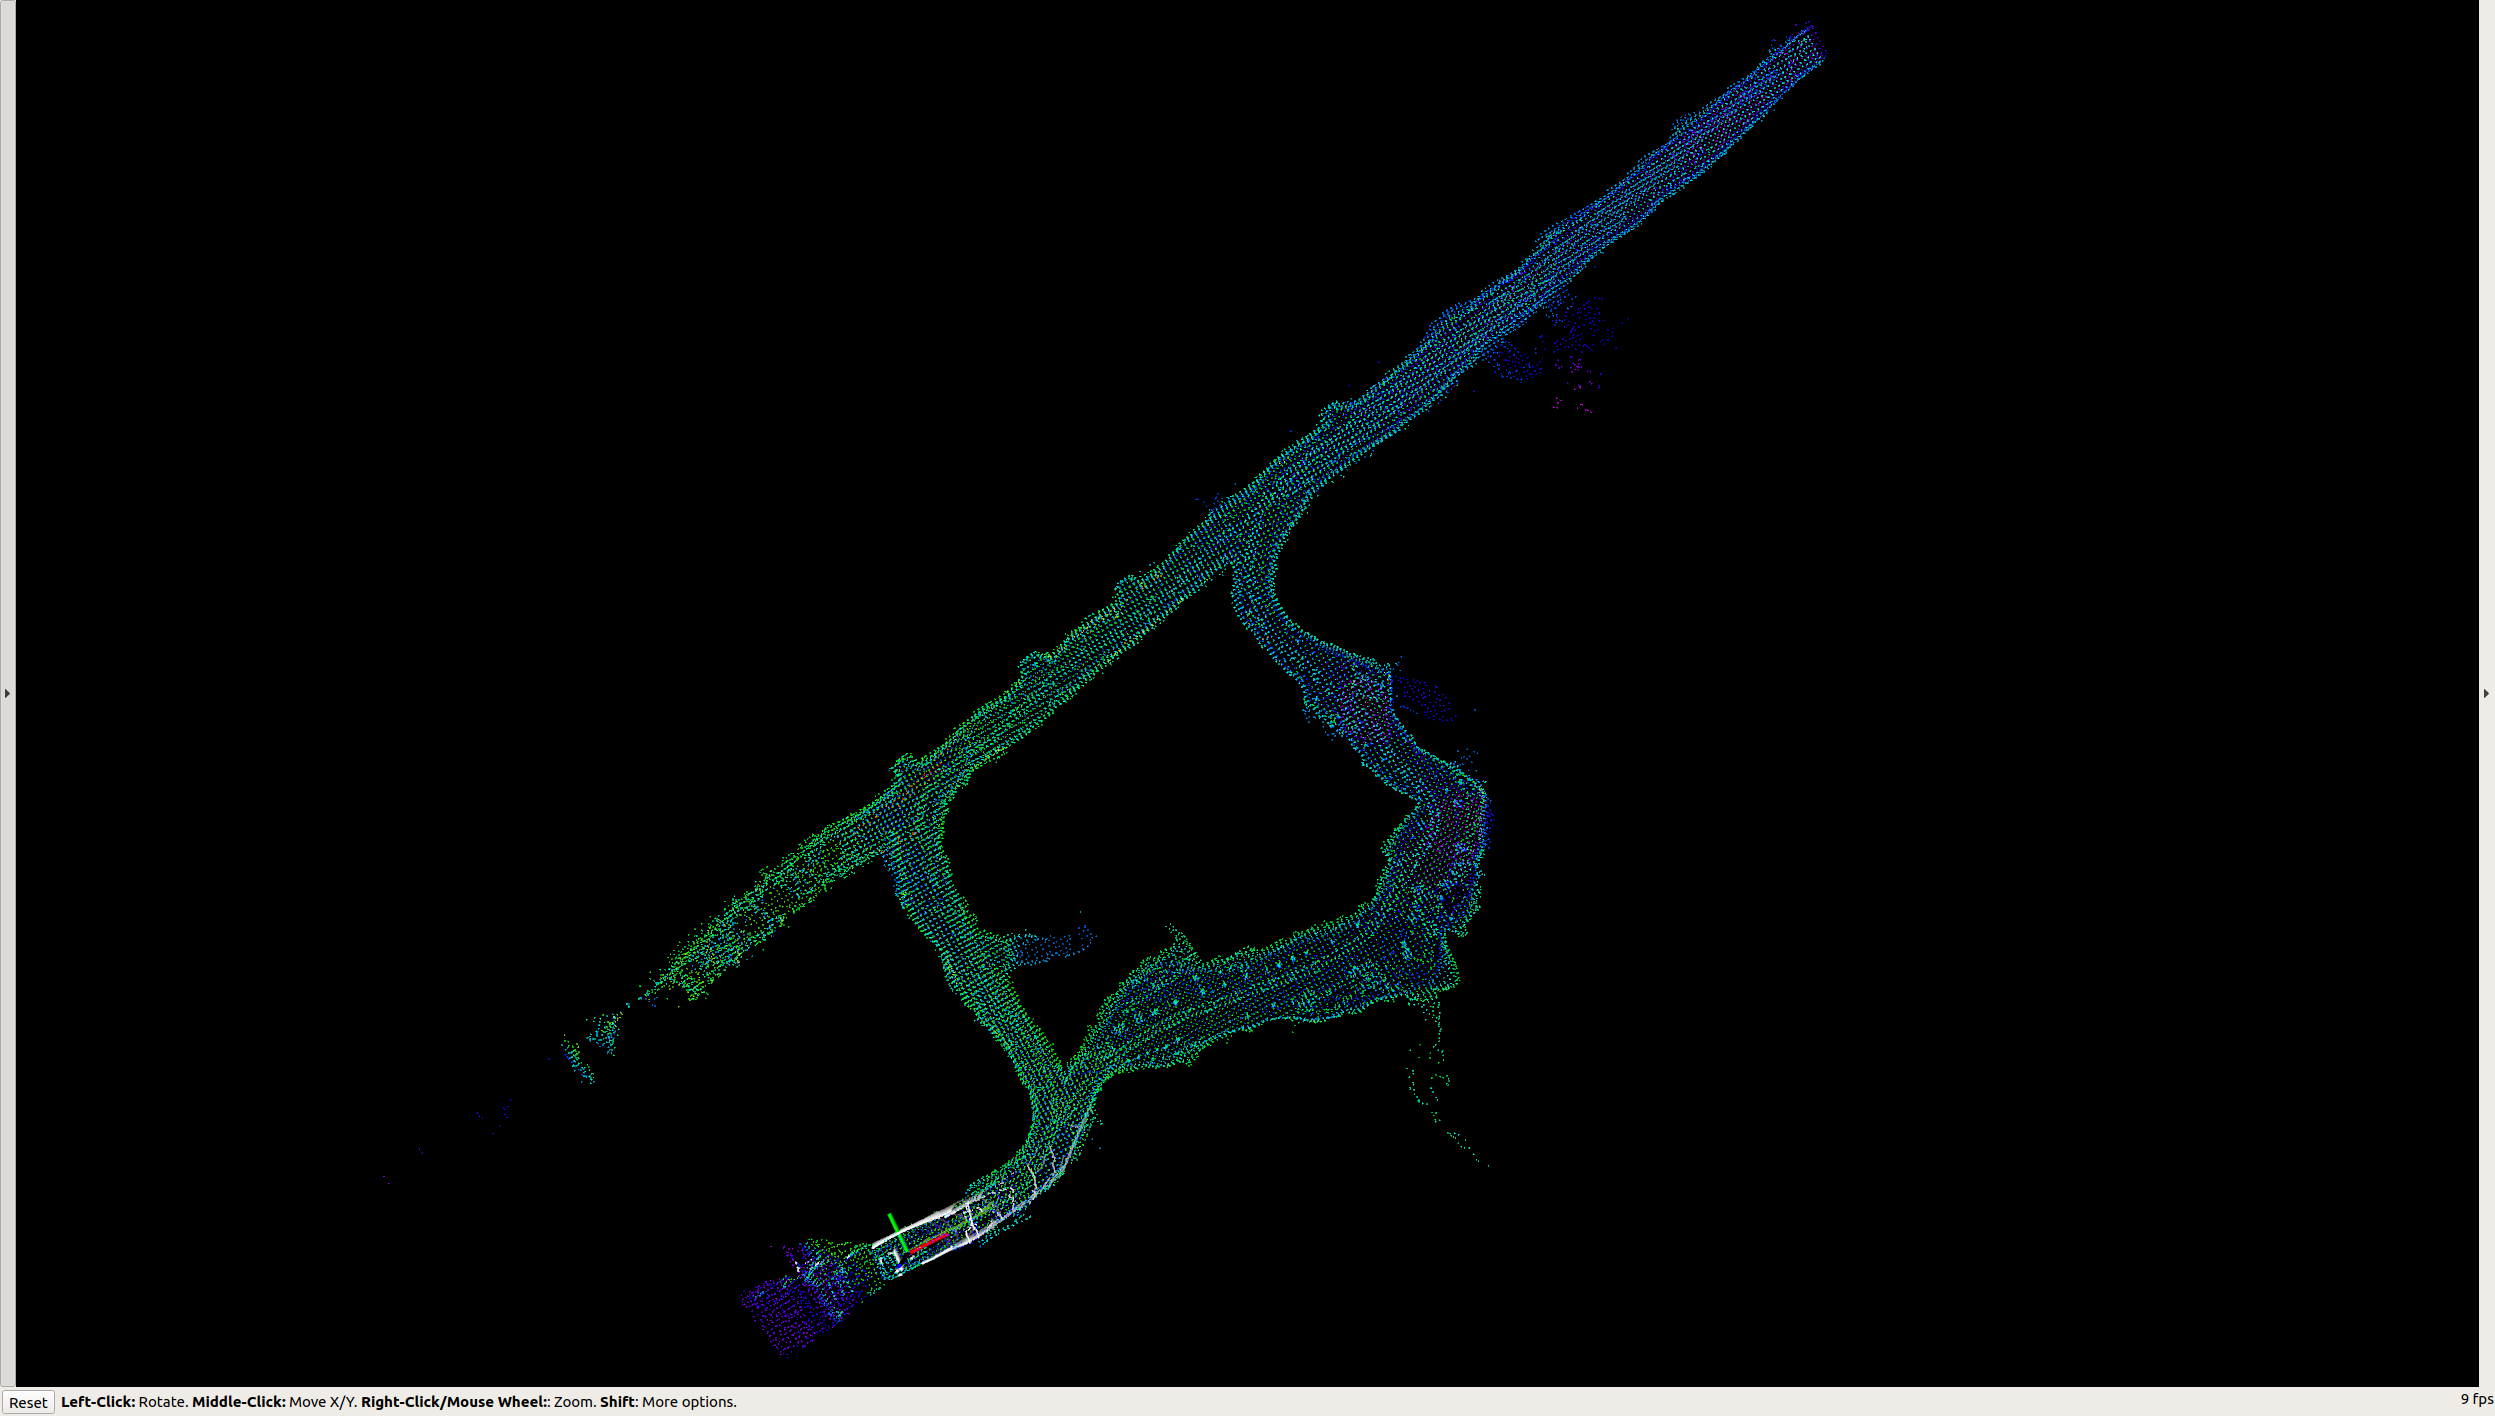
\includegraphics[width=\textwidth]{tour_ed_mine_1-00_1-50s.png}
		\caption{50\% points kept}
		\label{loam_xavier_50}
	\end{subfigure}	
	\caption[Visualization of LOAM running on an Xavier]{Visualization of LOAM running on an Xavier with different downsampling parameters, using pre-recorded data collected at the Tour-Ed Mine in Tarentum, PA. While the scan matching is correct when 50\% of points are discarded due to being able to register scans within 100 ms (fast enough to keep up with the 10 Hz data rate), the number of discarded points was deemed to be too severe.}
	\label{loam_xavier}
\end{figure}

In Figure \ref{loam_xavier_100}, the same configuration as the NUC on Mk. 0 was used. Severe misalignment is visible - the lower tunnel does not align correctly, and a secondary "ghost" tunnel is created. In Figure \ref{loam_xavier_75}, 75\% of the laser scanner's points are kept. This does result in better alignment, though the images of two tunnels are still clearly visible in the figure. Finally, in Figure \ref{loam_xavier_50}, only 50\% of the laser scanner's points are kept. In this environment, the point cloud alignment is successful, suggesting that the state estimate did not drift significantly. However, the requisite 50\% downsampling was deemed to be too significant, as it presented a high risk of misalignment under harsh motions or in feature-bare environments due to the low density of points. This experiment confirmed the initial hypothesis that, without significant optimization, the current autonomy stack would be unable to run on a single Xavier.

\subsection{State Estimation Sensor Selection}

Adhering to the requirement of rapid development (HWR1), the first candidates for state estimation sensors were selected to be those already validated to work with LOAM inside the Blue payload -- the Velodyne VLP-16 Puck LIDAR and an Xsens IMU. Alternative laser scanners, such as the Ouster OS1, were considered for use with LOAM, but the time required to tune and validate LOAM for these new sensors was deemed to be too much. The specific combination of sensors within the Blue payload has hundreds of hours of use and was proven to be reliable in a variety of environments. Achieving the same with new sensors would take prohibitively long and thus, the exact same sensor complement as the Blue payload was selected for state estimation within Mk. 0.

\subsection{Sensor Category Selection}

The selection of sensors for artifact detection was not as simple as that for state estimation. At this point in the competition, DARPA had not released a specific list of artifacts that would be used in the challenge, only 10 general categories \cite{tunnel_rules}. These categories were compared against the types of sensors which we believed could be integrated into Mk. 0 in a short amount of time. The utility of each type of sensor in detecting artifacts of each category was estimated according to the following guidelines, and is summarized in Table \ref{sensor_utility_categories}.

% TODO(vasua): Do I need to add more information about how I came up with this table?
\begin{description}
	\item[High] Artifacts of this category are expected to produce extreme sensor responses and be easy to distinguish.
	\item[Medium] Artifacts of this category are expected to be found in sensor data with moderate difficulty.
	\item[Low] Artifacts of this category are expected to be difficult or expensive to separate from sensor noise, perhaps due to a low response, or anticipated interference.
	\item[None] Artifacts of this category are expected to effect no response in sensors of this category.
\end{description}

% https://www.tablesgenerator.com/#
\begin{table}[]
	\centering
	\resizebox{\textwidth}{!}{%
		\begin{tabular}{lccccccc}
			\hline
			& \textbf{\begin{tabular}[c]{@{}c@{}}RGB\\ Camera\end{tabular}} & \textbf{\begin{tabular}[c]{@{}c@{}}Thermal\\ Camera\end{tabular}} & \textbf{\begin{tabular}[c]{@{}c@{}}Depth\\ Camera\end{tabular}} & \textbf{LIDAR} & \textbf{Microphone(s)} & \textbf{\begin{tabular}[c]{@{}c@{}}Wifi / Bluetooth\\ Scanning\end{tabular}} & \multicolumn{1}{l}{\textbf{Gas Sensor}} \\ \hline
			\textbf{Survivors}                  & High                                                          & High                                                              & High                                                            & Medium         & Low                    & None                                                                         & None                                    \\ \hline
			\textbf{Ingress / Egress Points}    & Medium                                                        & Low                                                               & High                                                            & Medium         & Low                    & None                                                                         & Low                                     \\ \hline
			\textbf{Electric Pumps}             & High                                                          & High                                                              & Low                                                             & Medium         & Medium                 & None                                                                         & None                                    \\ \hline
			\textbf{Backpacks}                  & High                                                          & None                                                              & Low                                                             & Low            & None                   & None                                                                         & None                                    \\ \hline
			\textbf{Valves}                     & High                                                          & None                                                              & Low                                                             & None           & None                   & None                                                                         & None                                    \\ \hline
			\textbf{Radios / Cell Phones}       & Low                                                           & Medium                                                            & Low                                                             & None           & Medium                 & High                                                                         & None                                    \\ \hline
			\textbf{Tools / Fire Extinguishers} & High                                                          & None                                                              & Low                                                             & None           & None                   & None                                                                         & None                                    \\ \hline
			\textbf{Power Sources}              & Medium                                                        & High                                                              & Medium                                                          & Medium         & None                   & None                                                                         & None                                    \\ \hline
			\textbf{Oxygen Level}               & None                                                          & None                                                              & None                                                            & None           & None                   & None                                                                         & High                                    \\ \hline
			\textbf{Gas Leaks}                  & None                                                          & Medium                                                            & None                                                            & None           & Medium                 & None                                                                         & High                                    \\ \hline
		\end{tabular}%
	}
	\caption[Estimated sensor utility for artifact detection]{Estimated utility of various sensor categories for DARPA provided artifact categories. These sensor categories were selected for being easy to integrate into the Mk. 0 payload. At this point in the competition, the specific list of artifacts for the Tunnel Circuit had not yet been released, forcing comparison against the overall list of categories instead.}
	\label{sensor_utility_categories}
\end{table}

Table \ref{sensor_utility_categories} indicates that while there is some redundancy across sensing categories in their speculated ability to detect various artifact categories, most of the sensor types have at least one artifact category that they alone would be highly likely to detect. For example, WiFi / Bluetooth scanning is the only sensing category rated as "High" utility in detecting radios / cell phones. Based on this table, Mk. 0 should contain at least some sort of RGB camera, thermal camera, depth camera, WiFi / Bluetooth scanner, and gas sensor in order to have a high chance of detecting each of the possible artifact categories. A LIDAR isn't required for object detection, but will necessarily be included for state estimation as described above. The microphone isn't strictly necessary to detect any particular artifact category, but could be useful for future studies. If possible, it would be included in the payload, but it was considered low priority and little attention was devoted to it. With the list of sensor types decided, experimentation began to determine specific sensors to use from each category in Mk. 0.

\subsection{RGB Camera Selection}

An RGB camera was the first sensor selected as the category offered highest overall utility across a variety of sensor categories. The first selection criteria for the camera was the interface type. Three possibilities were considered - CSI, Ethernet, and USB. CSI, capable of offering very high data rates with low latency, was the preferred interface. However, hardware and driver support for CSI cameras for the Xavier was still developing at this time, eliminating this option. Ethernet was considered for ease of integration. However, the larger size of Ethernet cameras and connectors, as well as the lower available bandwidth for multiple cameras forced this option to be eliminated as well. This left only USB for the camera interface, forcing it to be selected by default. USB 3.0 offers the data rates needed to interface with multiple cameras, but has the potential to suffer from high latency of and jitter in between frames due to multiple levels of hardware and software buffering.

After finalizing USB for the camera interface, two specific USB camera models were considered for use in Mk. 0. The first was the UI-3241LE-C-HQ by IDS Imaging, a bare camera board that we had familiarity with from successful use in other projects. The second was the Intel RealSense D435, selected for its inclusion of a stereo depth pair in a small form factor. When comparing the two cameras, in addition to the overall payload goals, there were a few camera-specific criteria used:
	
\begin{description}
	\item[Low light performance] The subterranean environments were expected to be dimly lit in general, and occasionally be completely dark. A camera with lower image noise in dark environments was preferred.
	\item[Synchronization ability] Given the expected utility of the RGB cameras, as well as for redundancy, it was anticipated that multiple cameras would be used on Mk. 0. A hardware synchronization mechanism between the cameras and other payload sensors (e.g. LIDAR) would help increase the accuracy of various software algorithms.
	\item[Shutter type] A global shutter was preferred over a rolling shutter due to the increased image quality under harsh camera motions, which was expected as a result of rough terrain.
\end{description}

To evaluate low light performance, the provided ROS \cite{quigley2009ros} drivers were used to capture images from cameras at their native or recommended resolutions (1280 x 1024 for the UI camera, and 848 x 480 for the RealSense) across a range of manually selected exposure and gain values with the camera framerates set to 30 fps. The images shown in Figure \ref{camera_comparison} contain images of the same scene from both cameras with 33 ms exposure time and the minimum and maximum gains supported by the drivers. Additionally, images of a similar scene were captured with autoexposure enabled in each camera.

\begin{figure}
	\centering
	\begin{subfigure}{0.32\textwidth}
		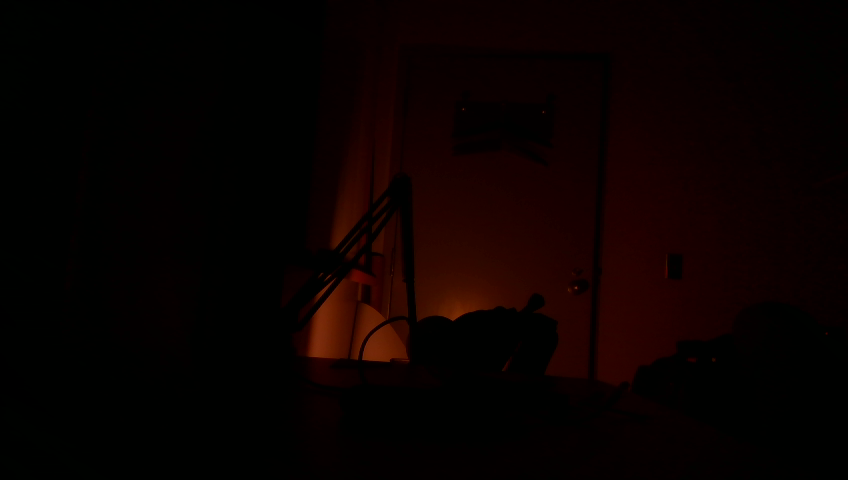
\includegraphics[width=\textwidth]{rs_img_33_ms_016.png}
		\caption{RealSense 33 ms exposure, minimum gain}
		\label{rs_img_33_ms_016}
	\end{subfigure}		
	\hfill
	\begin{subfigure}{0.32\textwidth}
		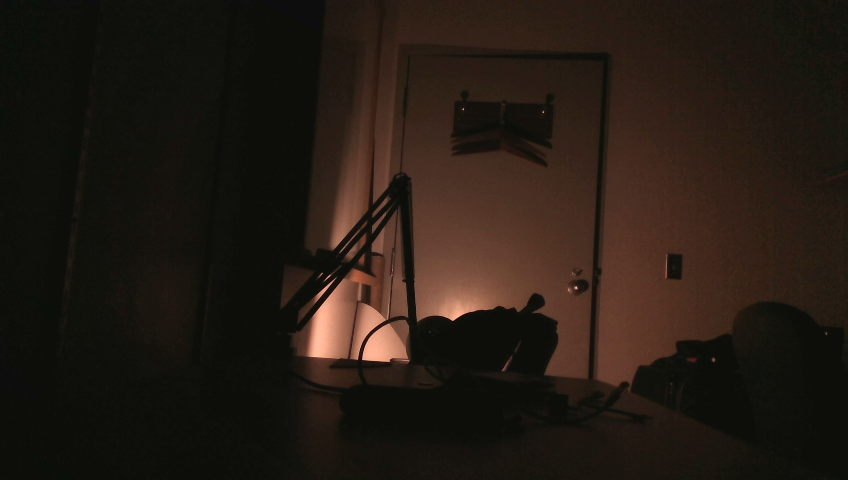
\includegraphics[width=\textwidth]{rs_img_33_ms_128.png}
		\caption{RealSense 33 ms exposure, maximum gain}
		\label{rs_img_33_ms_128}		
	\end{subfigure}
	\hfill
	\begin{subfigure}{0.32\textwidth}
		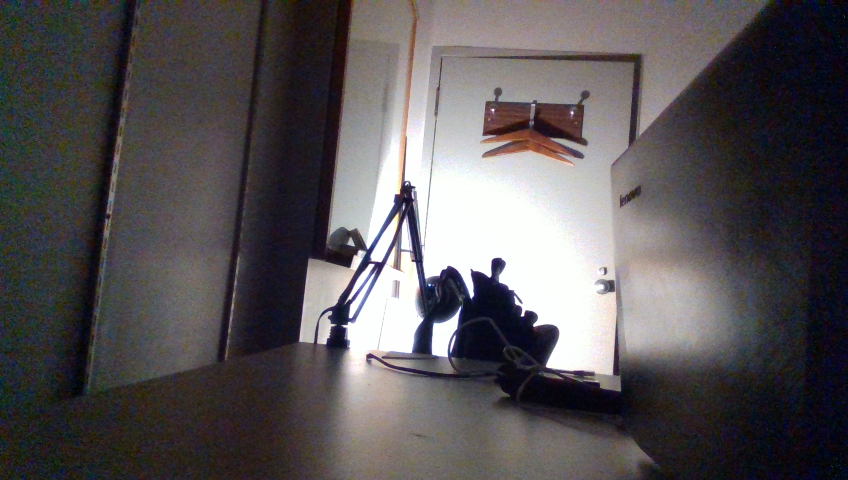
\includegraphics[width=\textwidth]{auto_realsense_2.png}
		\caption{RealSense automatic exposure, automatic gain}
		\label{auto_realsense_2}
	\end{subfigure}
	\\
	\begin{subfigure}{0.32\textwidth}
		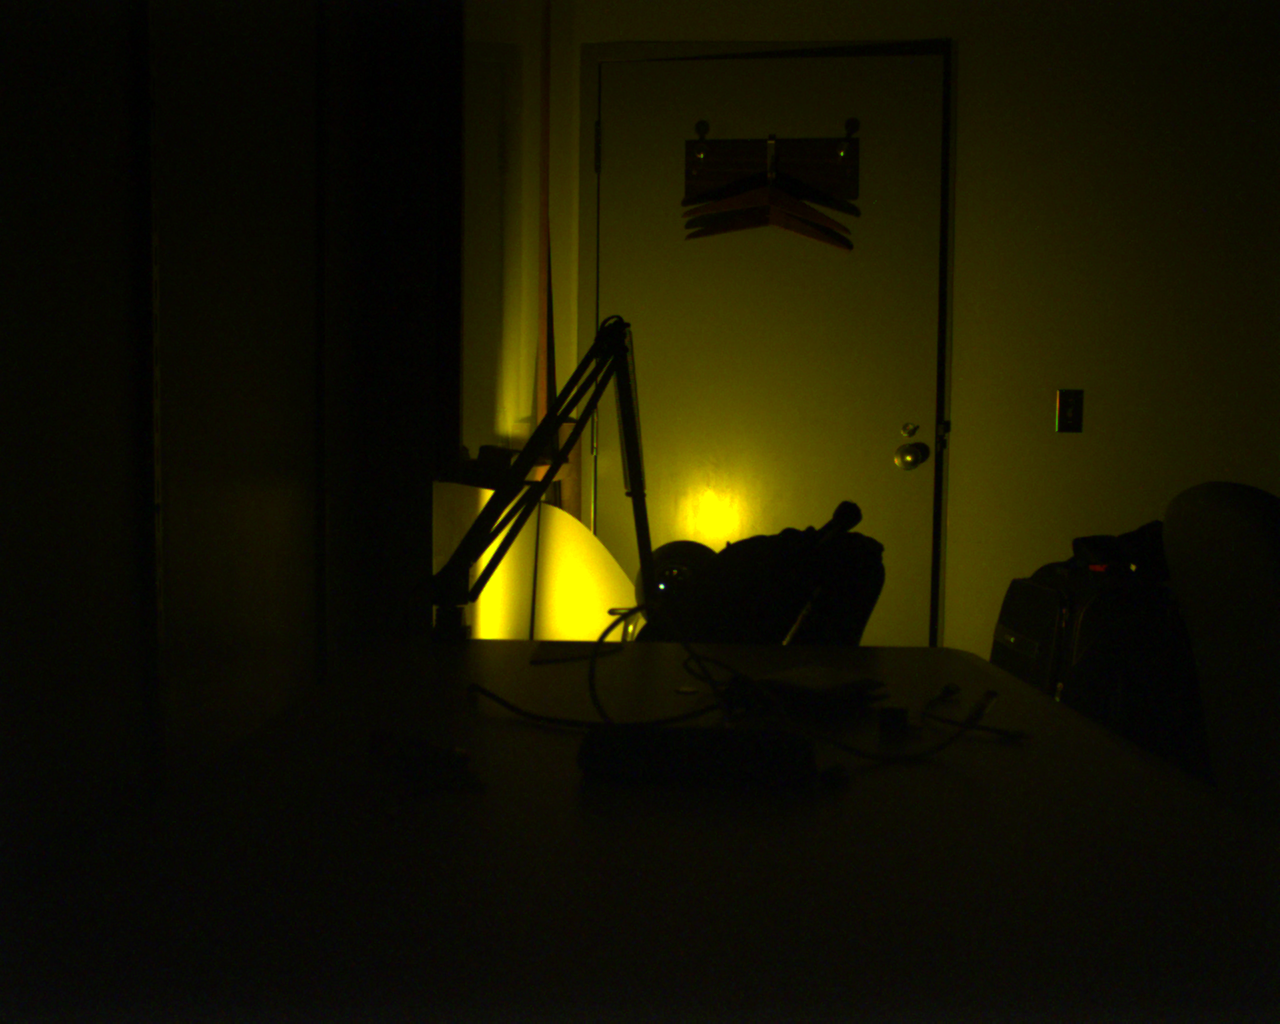
\includegraphics[width=\textwidth]{ui_img_33_ms_000.png}
		\caption{UI 33 ms exposure, minimum gain}
		\label{ui_img_33_ms_000}
	\end{subfigure}		
	\hfill
	\begin{subfigure}{0.32\textwidth}
		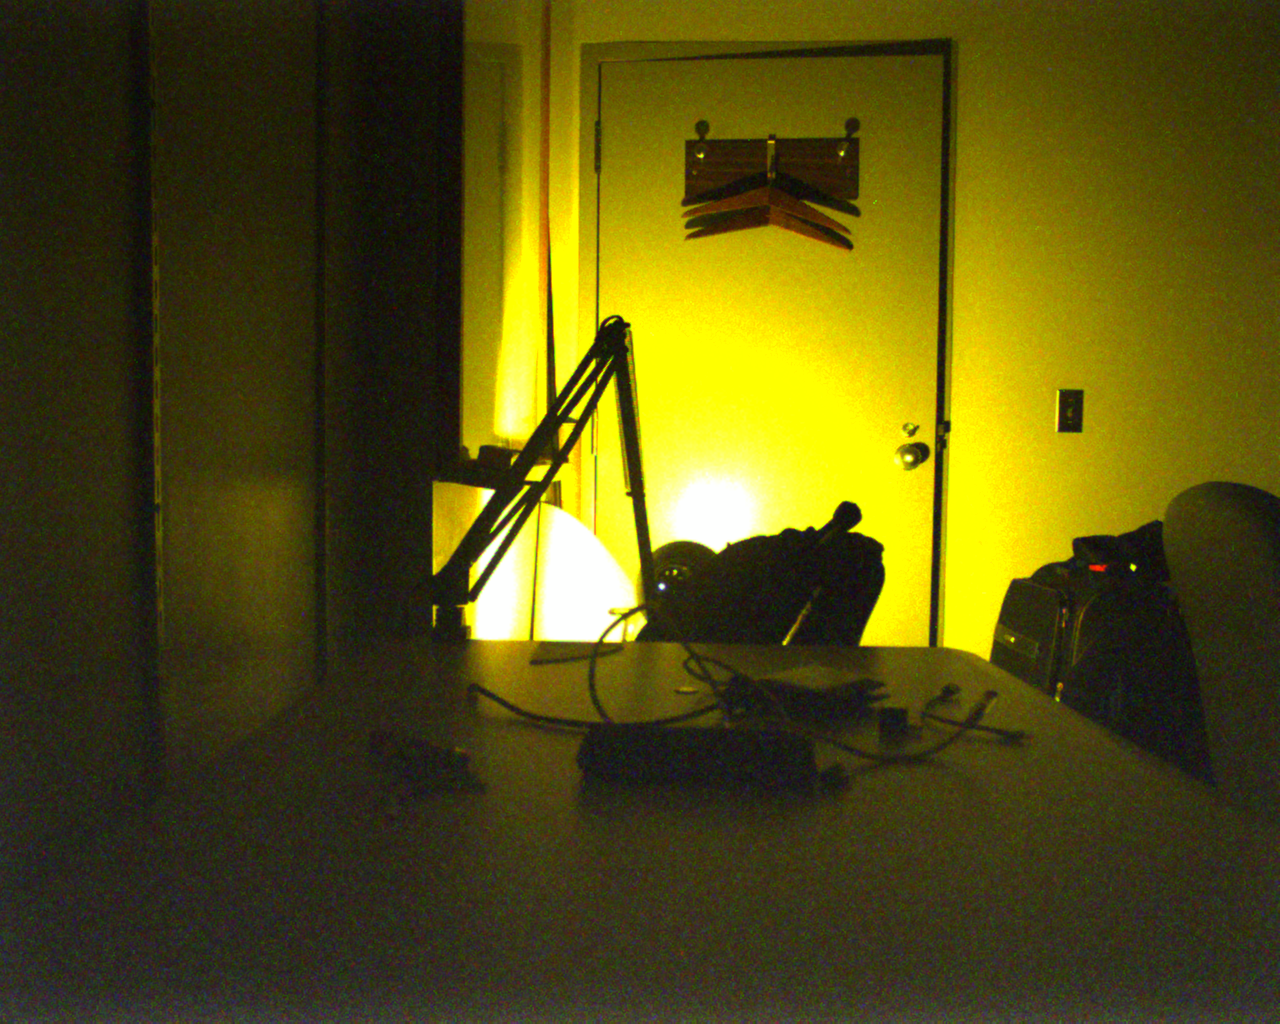
\includegraphics[width=\textwidth]{ui_img_33_ms_100.png}
		\caption{UI 33 ms exposure, maximum gain}
		\label{ui_img_33_ms_100}		
	\end{subfigure}
	\hfill
	\begin{subfigure}{0.32\textwidth}
		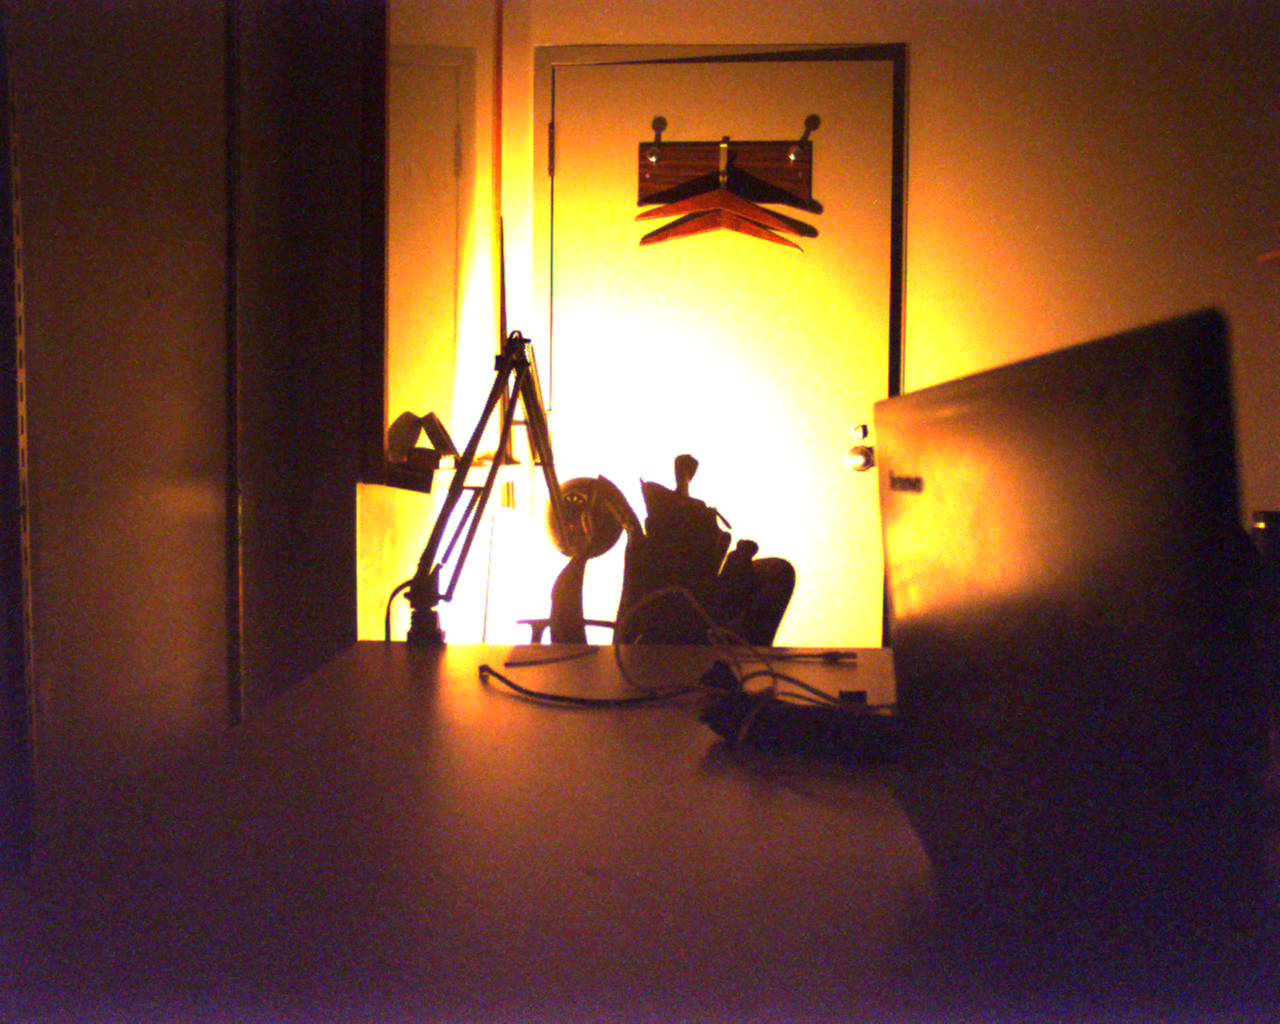
\includegraphics[width=\textwidth]{auto_ueye_2.png}
		\caption{UI automatic exposure, automatic gain}
		\label{auto_ueye_2}
	\end{subfigure}		
	\caption[RGB camera image quality comparison]{Comparison of image quality from UI-3241LE-C-HQ and RealSense D435 RGB cameras across a variety of gain values. Automatic exposure was limited to 33 ms due to a specified framerate of 30 fps for both cameras. It should be noted that after this experiment was performed, it was discovered that the RealSense firmware version used had a bug when setting manual gain which lowered the maximum possible gain value. The automatic gain feature did not have this bug, which could explain why the RealSense image with automatic gain in \ref{auto_realsense_2} appears significantly brighter.}
	\label{camera_comparison}
\end{figure}

With manual gain enabled on both cameras, the images from the RealSense RGB camera are less bright, but exhibit significantly less noise than the images from the UI camera. Additionally, the UI camera's image at maximum gain \ref{ui_img_33_ms_100} saturated in the center, while the RealSense image did not, suggesting a lower dynamic range on the UI camera. When autoexposure was enabled on both cameras (\ref{auto_realsense_2}, \ref{auto_ueye_2}), the RealSense exhibited comparable noise to the UI camera, but produced an image with colors more accurate to the actual scene.

When comparing synchronization ability, it appeared at first glance that both cameras supported external frame triggering, which allows frame capture to be driven by an external clock. This feature had previously been validated on the UI cameras in other lab projects. However, upon closer inspection it appeared that the external trigger for the RealSense module only applied to the depth module, and use of the external trigger would remove the synchronization between the RGB and depth modules on the RealSense camera. Similarly, when comparing shutter types, it appeared at first glance that both cameras had global shutters. This has also been previously validated on the UI cameras in other lab projects. However, further investigation revealed that the RealSense had a global shutter only for the 2 IR cameras used to compute depth, with the RGB camera instead having a rolling shutter.

After comparing the two camera models in these experiments, the RealSense D435 module was selected for use in Mk. 0. It was believed that the dramatic increase in low light image quality would outweigh the RGB camera rolling shutter and lack of external triggering. Additionally, the RealSense contains a depth module which eliminated the need for the selection of a separate depth camera. The RealSense also beat the UI camera in other payload requirements -- its price was less than half that of the UI camera (HWR5 cost sensitivity), had shorter lead times (HWR1 rapid development), and had an enclosure which would simplify keeping the payload environmentally robust compared to the bare UI camera board (HWR3 environmental robustness). A total of 4 RealSense modules would be used in Mk. 0, arranged approximately in a square to allow for easy mounting and to provide a nearly 360 degree horizontal field of view with the RGB cameras.

\subsection{Thermal Camera Selection}
The thermal camera selected for the Mk. 0 payload was the FLIR Boson 320 with a 92 degree HFOV. The Boson camera core was newly released at the time Mk. 0 was being developed, and its small form factor, along with ease of integration with the available USB interface, similar to the selected RGB cameras, made it a compelling option. The 92 degree HFOV model was selected specifically as it was believed the larger FOV would allow more artifacts to be visible during a deployment. Additionally, the 92 degree HFOV configuration is the only model to come with a special diamond-like coating which is qualified against harsh abrasion. This allowed us to place the camera in Mk. 0. without a special protective window, which would have been otherwise difficult to do due to the expensive and specific type of glass needed. Other thermal camera options were briefly considered, but the FLIR product was ultimately selected due to familiarity and successful use of some of their other products in other projects. An example highlighting the utility of thermal cameras in fog is shown in Figure \ref{fog_comparison}.

\begin{figure}
	\centering
	\begin{subfigure}{0.45\textwidth}
		\centering
		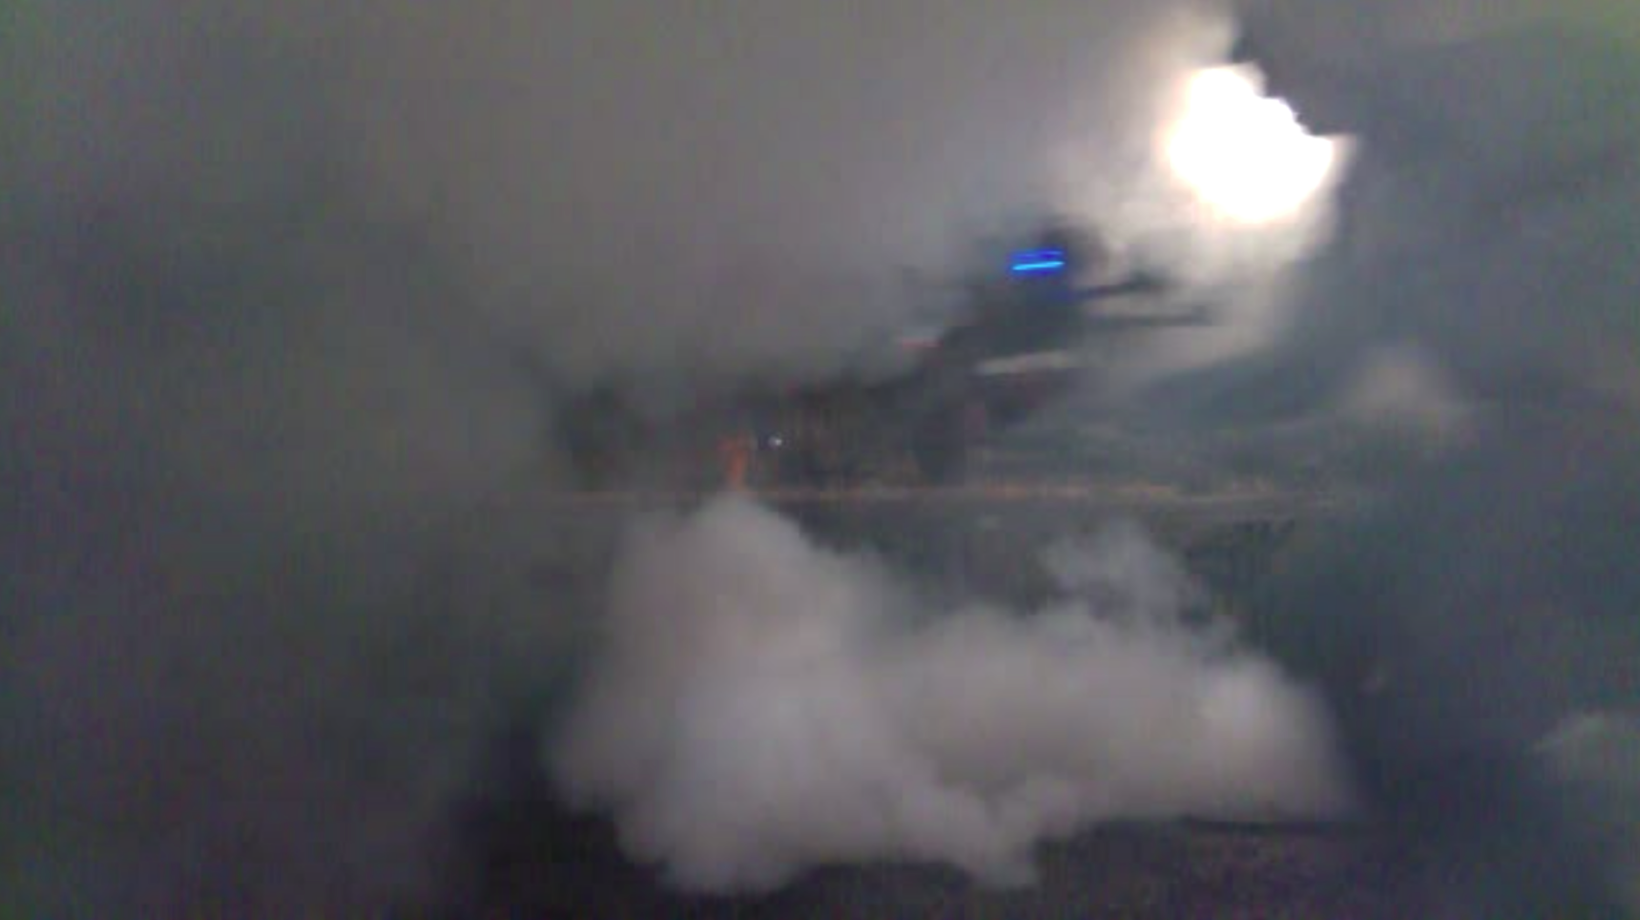
\includegraphics[width=\textwidth,height=4cm,keepaspectratio]{rgb_fog.png}
		\caption{RGB Image (RealSense D435)}
		\label{rgb_fog}
	\end{subfigure}
	\hfill
	\begin{subfigure}{0.45\textwidth}
		\centering
		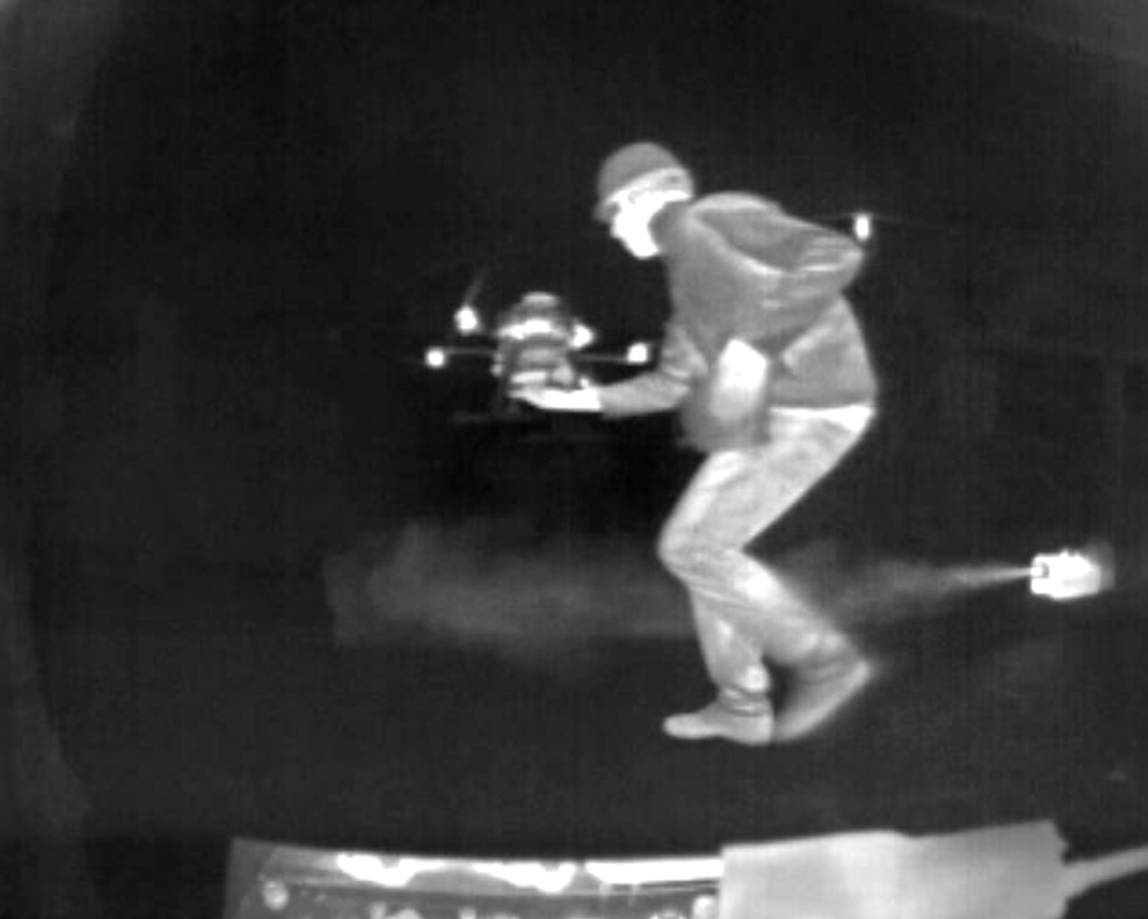
\includegraphics[width=\textwidth,height=4cm,keepaspectratio]{thermal_fog.png}
		\caption{Thermal Image (FLIR Boson 320)}
		\label{thermal_fog}
	\end{subfigure}		
	\caption[Comparison of RGB and Thermal cameras in fog]{The figure shows a scene containing a drill and a person carrying a drone in heavy fog. The RGB camera is able to see the drill in the parts of the image without fog, but is unable to easily distinguish the human. The thermal camera is able to clearly show the human through the fog but does not register a strong response for the drill.}
	\label{fog_comparison}
\end{figure}

\subsection{Microphone Selection}
The microphone was not identified to be a critical sensor in Table \ref{sensor_utility_categories}, and thus its selection was not dedicated significant resources. The "Insten VOIP/SKYPE Mini Flexible Microphone for VOIP/SKYPE - Black" was purchased from Amazon.com and was intended to be connected to NUC. After being unable to record audio information with the microphone connected to the NUC, it was discovered that the NUC's 3.5mm audio jack was a combination headset and microphone jack. A jack splitter was purchased and used to connect the microphone to the NUC successfully. Proof-of-concept driver support was added to record audio from the microphone, but the recorded audio data was never utilized.

\subsection{WiFi / Bluetooth Scanning Hardware Selection}
The NUC used inside the Mk. 0 payload contains an Intel Dual Band Wireless AC + Bluetooth 9560 module, capable of performing both WiFi and Bluetooth scanning simultaneously. The module is not used for other tasks on the robots as their wireless functionality is achieved with other, more specialized mesh hardware. Utilizing the hardware already contained on the NUC meant a reduced component count and easier integration, which was consistent with the payload goals (HWR1 rapid development, HWR5 cost sensitivity), making it a simple choice. Adapters were attached to the 9560 module to convert the dual MHF IV connectors to RP-SMA, allowing multiple antenna configurations to be easily tested without risking damage to the fragile MHF IV connectors on the module.

\subsection{Gas Sensor Selection}

With no specific information provided by DARPA about the gas leak artifact, we chose to focus our preliminary efforts on detecting oxygen levels. The Grove Oxygen Gas Sensor from SeeedStudio was selected for its low price and apparent ease of integration through an analog interface. However, the sensor did not report the expected oxygen concentration values (approximately 21\%) using the equations from the provided documentation. The decision was made to continue with Mk. 0 payload development without a gas sensor for the time being, with the intention of exploring alternative options and updating the payload as necessary in the future as more information was released. However, no further work was done with gas sensors as it was revealed soon afterwards that the Tunnel Circuit would not contain any gas artifacts.

%TODO(vasua): Mention SSD selection. Maybe put it in supporting components instead.
	
\subsection{Lighting Hardware Selection}

While the low light performance of the RealSense RGB camera was considered acceptable, adding additional lighting to the payload would enable images to be captured with lower noise, as well as allow for lower exposure times which could help decrease motion blur. Additional lighting would also be required for successful object detection in completely dark environments, which were to be expected in subterranean environments. To provide this additional lighting, the 5000K LED from the Opulent XHP70A series of LEDs, mounted on a starboard for ease of integration, was selected. This particular LED was chosen because it has the highest rated luminous flux of all LEDs we were able to find with the starboard form factor at the target voltage of 12V. 2 LEDs would be used per camera for increased brightness, as well as some redundancy in the case of failure of one of the LEDs.

After selecting the LEDs, the original intent was to synchronize and flash each pair of LEDs with the frame exposure of its associated RGB camera. Doing so would require some way of determining when the frame exposure was happening. The RealSense D435 has an expansion header with 9 pins, many of which were undocumented at the time. 1 of these pins was documented as being intended for synchronization of multiple depth modules, but no further details were provided. While probing the other undocumented pins with an oscilliscope did not reveal any signals that could be used to flash the LEDs, it revealed that the depth synchronization pin is simply a 1.8V 50$\mu$s pulse. The RealSense documentation was shortly updated to indicate that this pulse occurred slightly after the end of the depth frame exposure. Documentation also revealed that in normal operation, with the RGB camera acting as the master for the entire RealSense module, the start of the depth and RGB frame times should be synchronized. Using this information, the following equation is derived, allowing the time of the start of the next RGB camera exposure to be calculated from the start of the depth trigger:
	
\begin{equation} \label{led_flashing_eq}
	t_{rgb+1} = t_{depth} - t_{delay} - t_{exposure} + t_{frame}
\end{equation}

where $t_{rgb+1}$ is the start of exposure of the next RGB frame, $t_{depth}$ is the time of the start of the depth pulse, $t_{delay}$ is the delay between the end of depth exposure and the start of the depth pulse, $t_{exposure}$ is the exposure time of the depth frame, and $t_{frame}$ is the period of the camera frames. $t_{delay}$ was estimated by looking at the difference between the end of the depth projector control signal (in green) and the start of the depth pulse (in yellow), as shown in Figure \ref{realsense_delay}, and was set to 100 $\mu$s. The magnitude of this delay is negligible compared to $t_{frame}$ and $t_{exposure}$, which are in the tens of milliseconds, but it is provided for completeness.

\begin{figure}
	\centering
	\begin{subfigure}{0.32\textwidth}
		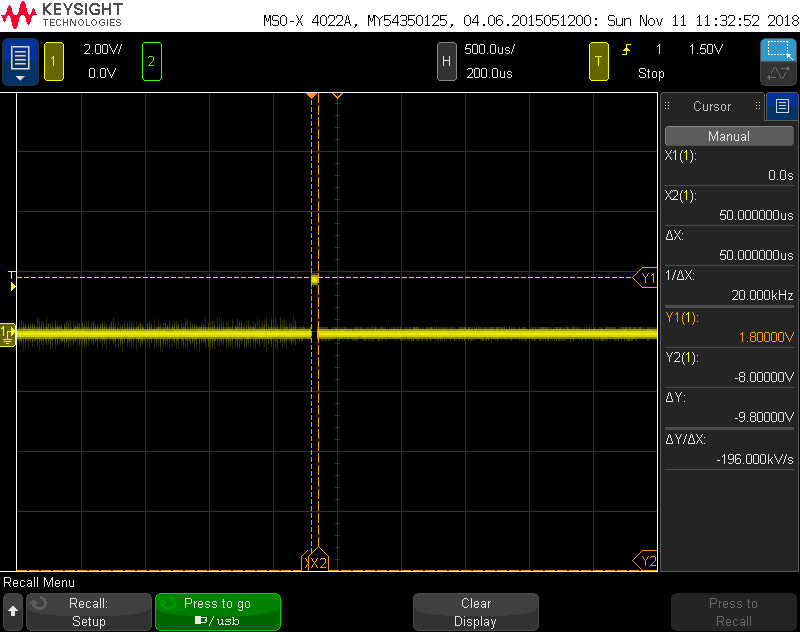
\includegraphics[width=\textwidth]{realsense_trigger.png}
		\caption{1.8V 50$\mu$s pulse after depth frame}
		\label{realsense_trigger}
	\end{subfigure}		
	\hfill
	\begin{subfigure}{0.32\textwidth}
		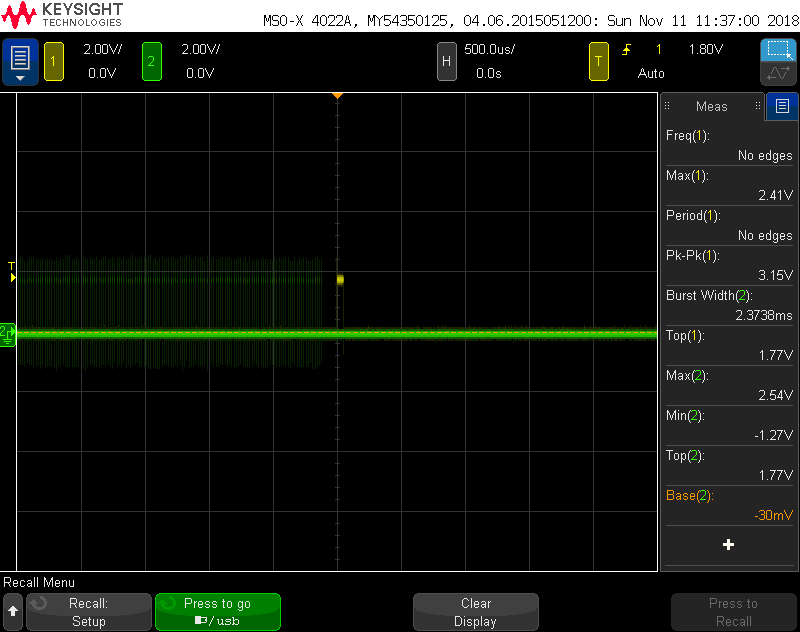
\includegraphics[width=\textwidth]{realsense_delay.png}
		\caption{Measurement used to estimate $t_{delay}$}
		\label{realsense_delay}		
	\end{subfigure}
	\hfill
	\begin{subfigure}{0.32\textwidth}
		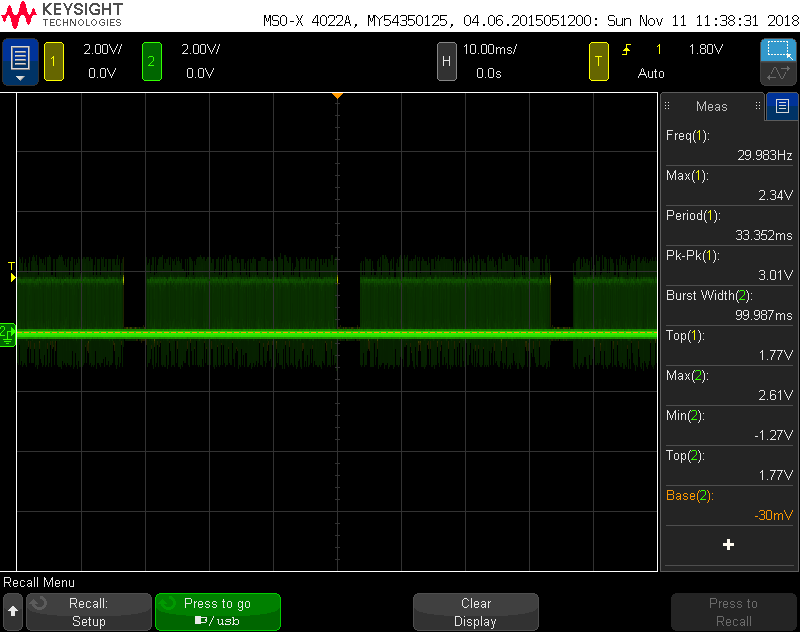
\includegraphics[width=\textwidth]{multiple_triggers.png}
		\caption{Depth triggers generated for each frame}
		\label{multiple_triggers}
	\end{subfigure}	
	\caption[Oscilliscope measurements of RealSense D435 depth trigger]{Oscilliscope measurements of RealSense D435 depth trigger. The depth pulse is shown in yellow. The IR projector control signal, active for the duration of the depth frame, is shown in green. The figures depict the depth trigger signal which occurs slightly after the end of exposure of every depth frame, and can be used to synchronize the flashing of LEDs with the RealSense RGB camera image exposure.}
	\label{realsense_scope}
\end{figure}	

To implement the LED flashing, the depth pulse was wired into an interrupt pin on a microcontroller. The interrupt triggered a timer which would sleep until the start of the next RGB frame exposure, as calculated in \ref{led_flashing_eq}. At the start of the frame, the LEDs would be turned on, and a second timer was initialized to turn the LEDs off after a specified period. The LEDs were controlled with the LED driver's dimming functionality, set to either maximum brightness or off. The LED driver selected was the BuckBlock A009, a constant current LED driver capable of supplying 2.1A at up to 16V, which was sufficient to drive 2 of the selected LEDs at their rated brightness when wired in parallel. 

Unfortunately, the LED flashing created artifacts in the RGB camera image. The streaking visible in Figure \ref{strobe_images} is believed to be a result of the rolling shutter on the RGB camera modules. Though each row in the RGB image may be exposing for less time than the frame period, the rows are being scanned sequentially, over the duration of the frame period. This means that if the LEDs are on for less time than the frame period, certain rows (depending on the exposure time set by the autoexposure algorithm) will not expose while the LEDs are on, resulting in a dark streak as seen in the figure. The specific dark rows are a function of the phase offset between the LED pulse and the rolling shutter.

The black streaks visible in Figure \ref{strobe_images} led to the decision that LED flashing would not be integrated for Mk. 0. The LEDs would instead be left on constantly, powered by a 12V constant voltage source rather than a separate LED driver. This would burn more power and in turn generate more heat on the payload, but would result in higher quality images to be used by other components in the pipeline. The connection of the voltage source to the LEDs was controlled by a switch to allow a user to disable the bright LEDs when not in use.
		
\begin{figure}
	\centering
	\begin{subfigure}{0.32\textwidth}
		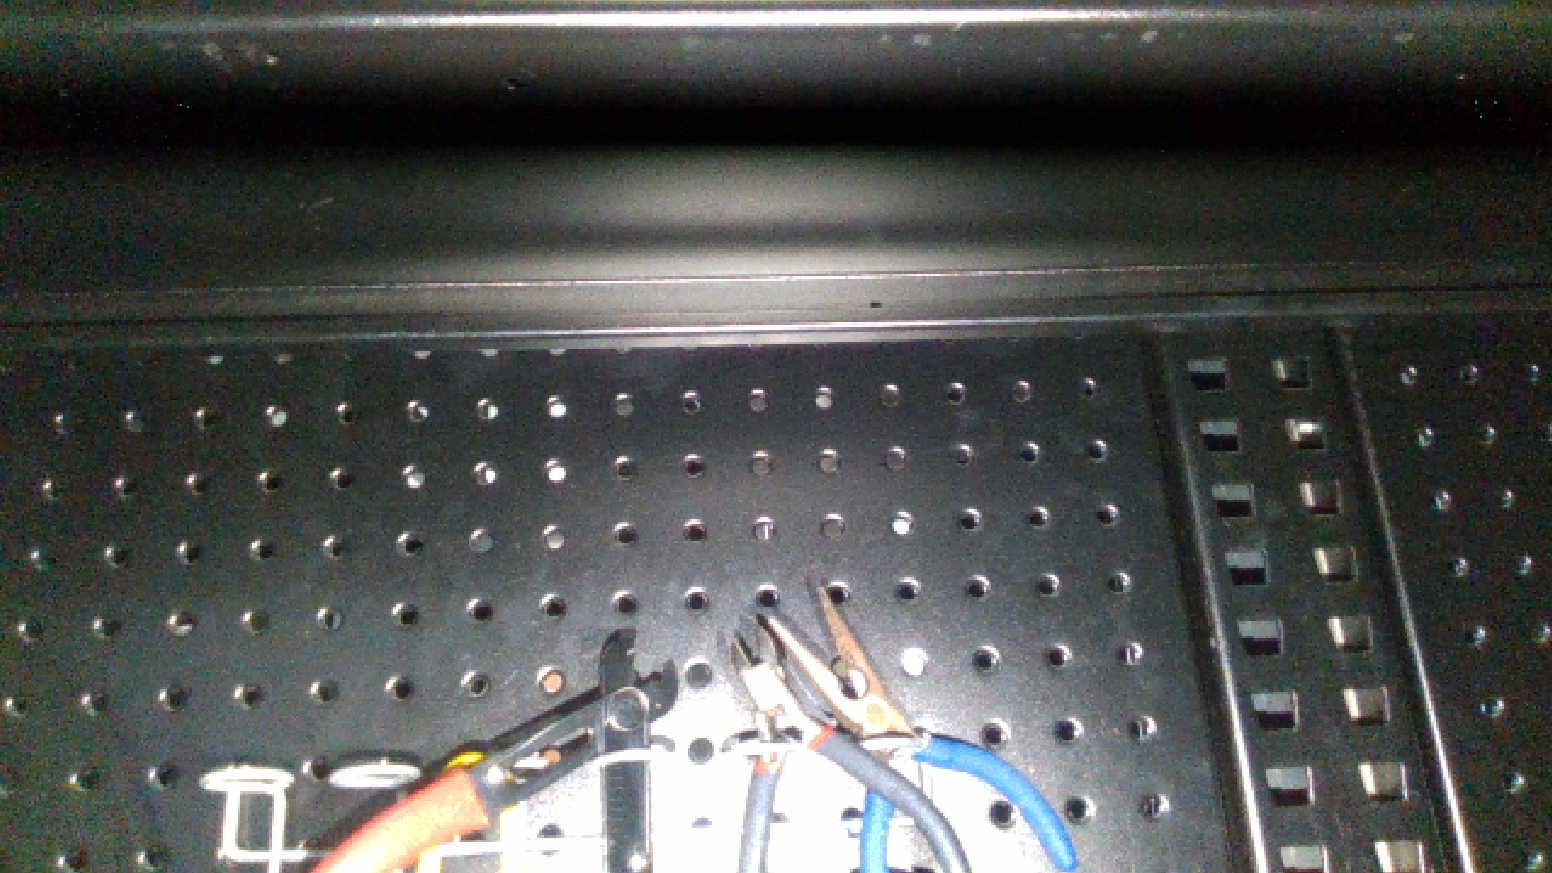
\includegraphics[width=\textwidth]{strobe_1.png}
		\caption{Top dark stripe}
		\label{strobe_top}
	\end{subfigure}		
	\hfill
	\begin{subfigure}{0.32\textwidth}
		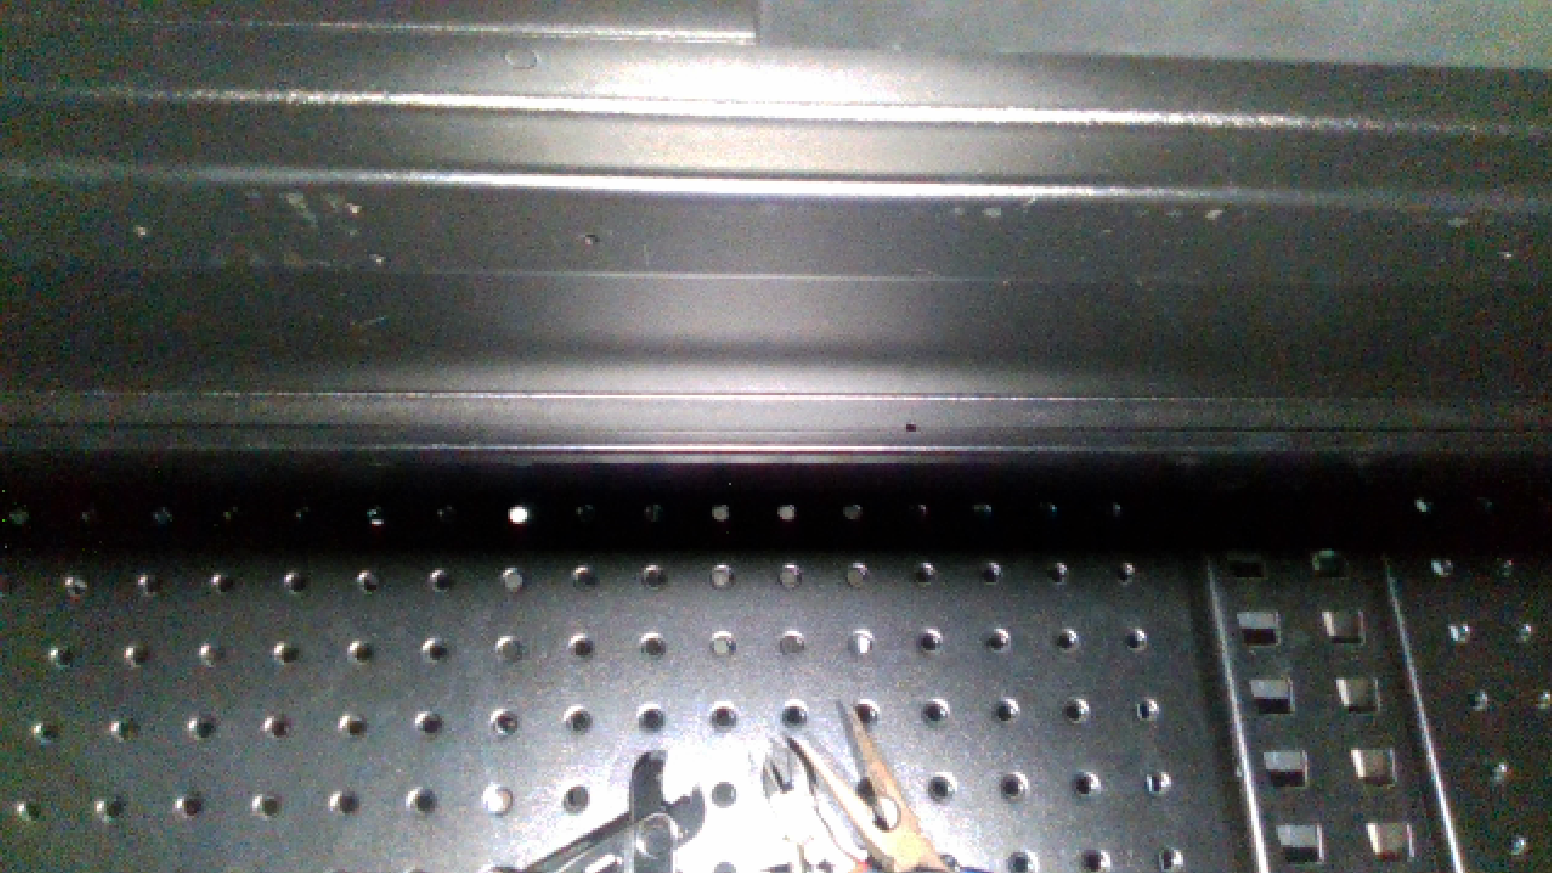
\includegraphics[width=\textwidth]{strobe_4.png}
		\caption{Middle dark stripe}
		\label{strobe_middle}		
	\end{subfigure}
	\hfill
	\begin{subfigure}{0.32\textwidth}
		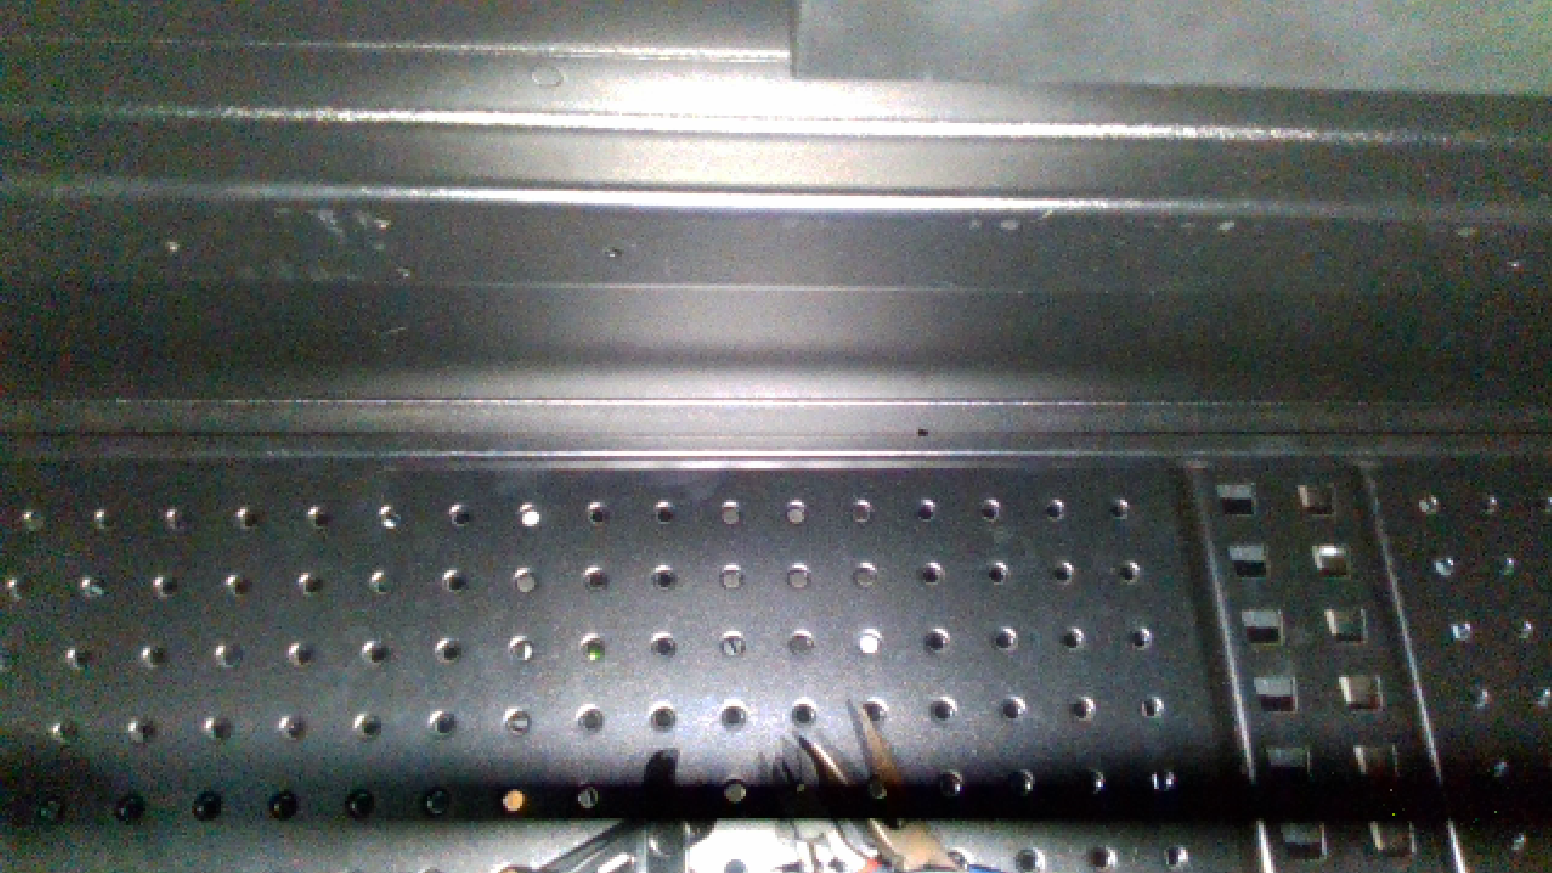
\includegraphics[width=\textwidth]{strobe_6.png}
		\caption{Bottom dark stripe}
		\label{strobe_bottom}
	\end{subfigure}	
	\caption[Dark lines in RealSense RGB images with LED flashing]{Dark lines are generated in the RealSense RGB images as a result of flashing the LEDs. The different locations of the dark stripes are caused by phase offsets between the LED pulse and the frame exposures. The phase offset was controlled by modifying $t_{delay}$ in Equation \ref{led_flashing_eq} to be between 0 and the frame period $t_{frame}$.}
	\label{strobe_images}
\end{figure}	

\subsection{Networking Hardware Selection}
Inside the Mk. 0 payload, the NUC, Xavier, and LIDAR are all connected together via Ethernet. Additionally, an Ethernet port is exposed from the payload to enable data output. In the interest of compactness, a GigEthos Lite board from Gadgetsmyth, which promised to be a very light and small gigabit Ethernet switch, was used originally. The board was successfully used inside the Mk. 0 for a few months after the initial assembly, but suddenly experienced an unexpected failure during normal operation. At that time, the GigEthos Lite board was replaced with a stripped down commodity TP-Link gigabit Ethernet switch. The failure of the GigEthos Lite board is currently believed to be caused due to insufficient cooling inside the payload, and it is believed that the larger surface area of the TP-Link board has helped prevent it from suffering from the same thermal issues.

\subsection{USB Hardware Selection}
The Mk. 0 payload contains a total of 6 USB sensors - 4 RealSense cameras, 1 thermal camera, and 1 IMU. All of the sensors except the IMU plug into the Xavier. However, the Xavier carrier board used (the developer kit carrier board) only has 3 USB ports - 2x 3.1 Gen 2 (10 Gb/s) Type C ports, and 1x 3.1 Gen 1 (5 Gb/s) Type A port. This meant that a USB hub was necessary for Mk. 0. The HB31C4AB hub from StarTech.com was selected as it was the only USB Type C hub with 4x USB Type A inputs capable of 10 Gb/s. Though the RealSense D435 cameras are only USB 3.1 Gen 1 (5 Gb/s) devices, which would limit the bus to 5 Gb/s, this 10 Gb/s capable USB hub was selected to permit future expansion and upgrades.

When thinking about USB devices, it was also decided to expose one of the USB Type C connectors from each of the two computers inside Mk. 0 as a bulkhead connector. This would allow for faster data transfers than would be possible over the existing gigabit Ethernet interface. Additionally, the exposed connectors made it possible to use any commodity USB Type C hub to break out display, keyboard, and mouse interfaces for easier debugging than would be possible via a headless connection.

\subsection{Power Hardware Selection}

The selected components for the Mk. 0 payload have a variety of different input voltage ranges and power requirements. For example, the NUC is rated for supply voltages between 12V and 19V, though was shown in prior experience to be unstable at voltages below 13V. The LEDs could be given no more than 12V without exceeding the maximum current specifications. It was determined that all components in the payload could be powered with one of two supply voltages - 12V and 18V. Unfortunately, neither of these voltages are available on the ground robot platforms. Even if they were, placing such strict requirements on the available voltages reduces the modularity of the payload, which is in direct conflict with one of the major design goals. It was instead decided to design the payload to accept a nominal 24V supply, which is available on all three platforms, and internally regulate it down to the desired voltages of 12V and 18V. The ground robots offer a regulated 24V line, while the raw battery voltage from the 6S LiPo (22.2V - 25.2V) can be used on the drone platform.

\section{Mk. 0 Assembly}

The enclosure for Mk. 0 was designed in parallel with the component selection process. Heat dissipation was an important design consideration, as the payload was expected to draw more than 250W at full load. This led to the entire body of the payload being made of aluminum, a metal with relatively high thermal conductivity. Many of the components were then attached directly to the body with thermal paste to ensure optimal heat dissipation. The body itself is a cube constructed of three major pieces - a top plate, a bottom plate, and a single unit comprising all of the side panels. This construction allows for rapid entry into the payload by just removing the top plate. The panels were designed to be simple enough to manufacture in-house or outsourced to a commercial waterjet facility with rapid turnaround. Some pictures from the initial assembly steps are shown in Figure \ref{mk_0_assembly}. After assembling Mk. 0 for the first time, it became apparent that it is too large, at approximately 8" in each dimension without the LIDAR, and too heavy, at nearly 20 lbs, to fly on the drone. A separate, simplified version of Mk. 0 would be needed for the drone.

\begin{figure}
	\centering
	\begin{subfigure}{0.32\textwidth}
		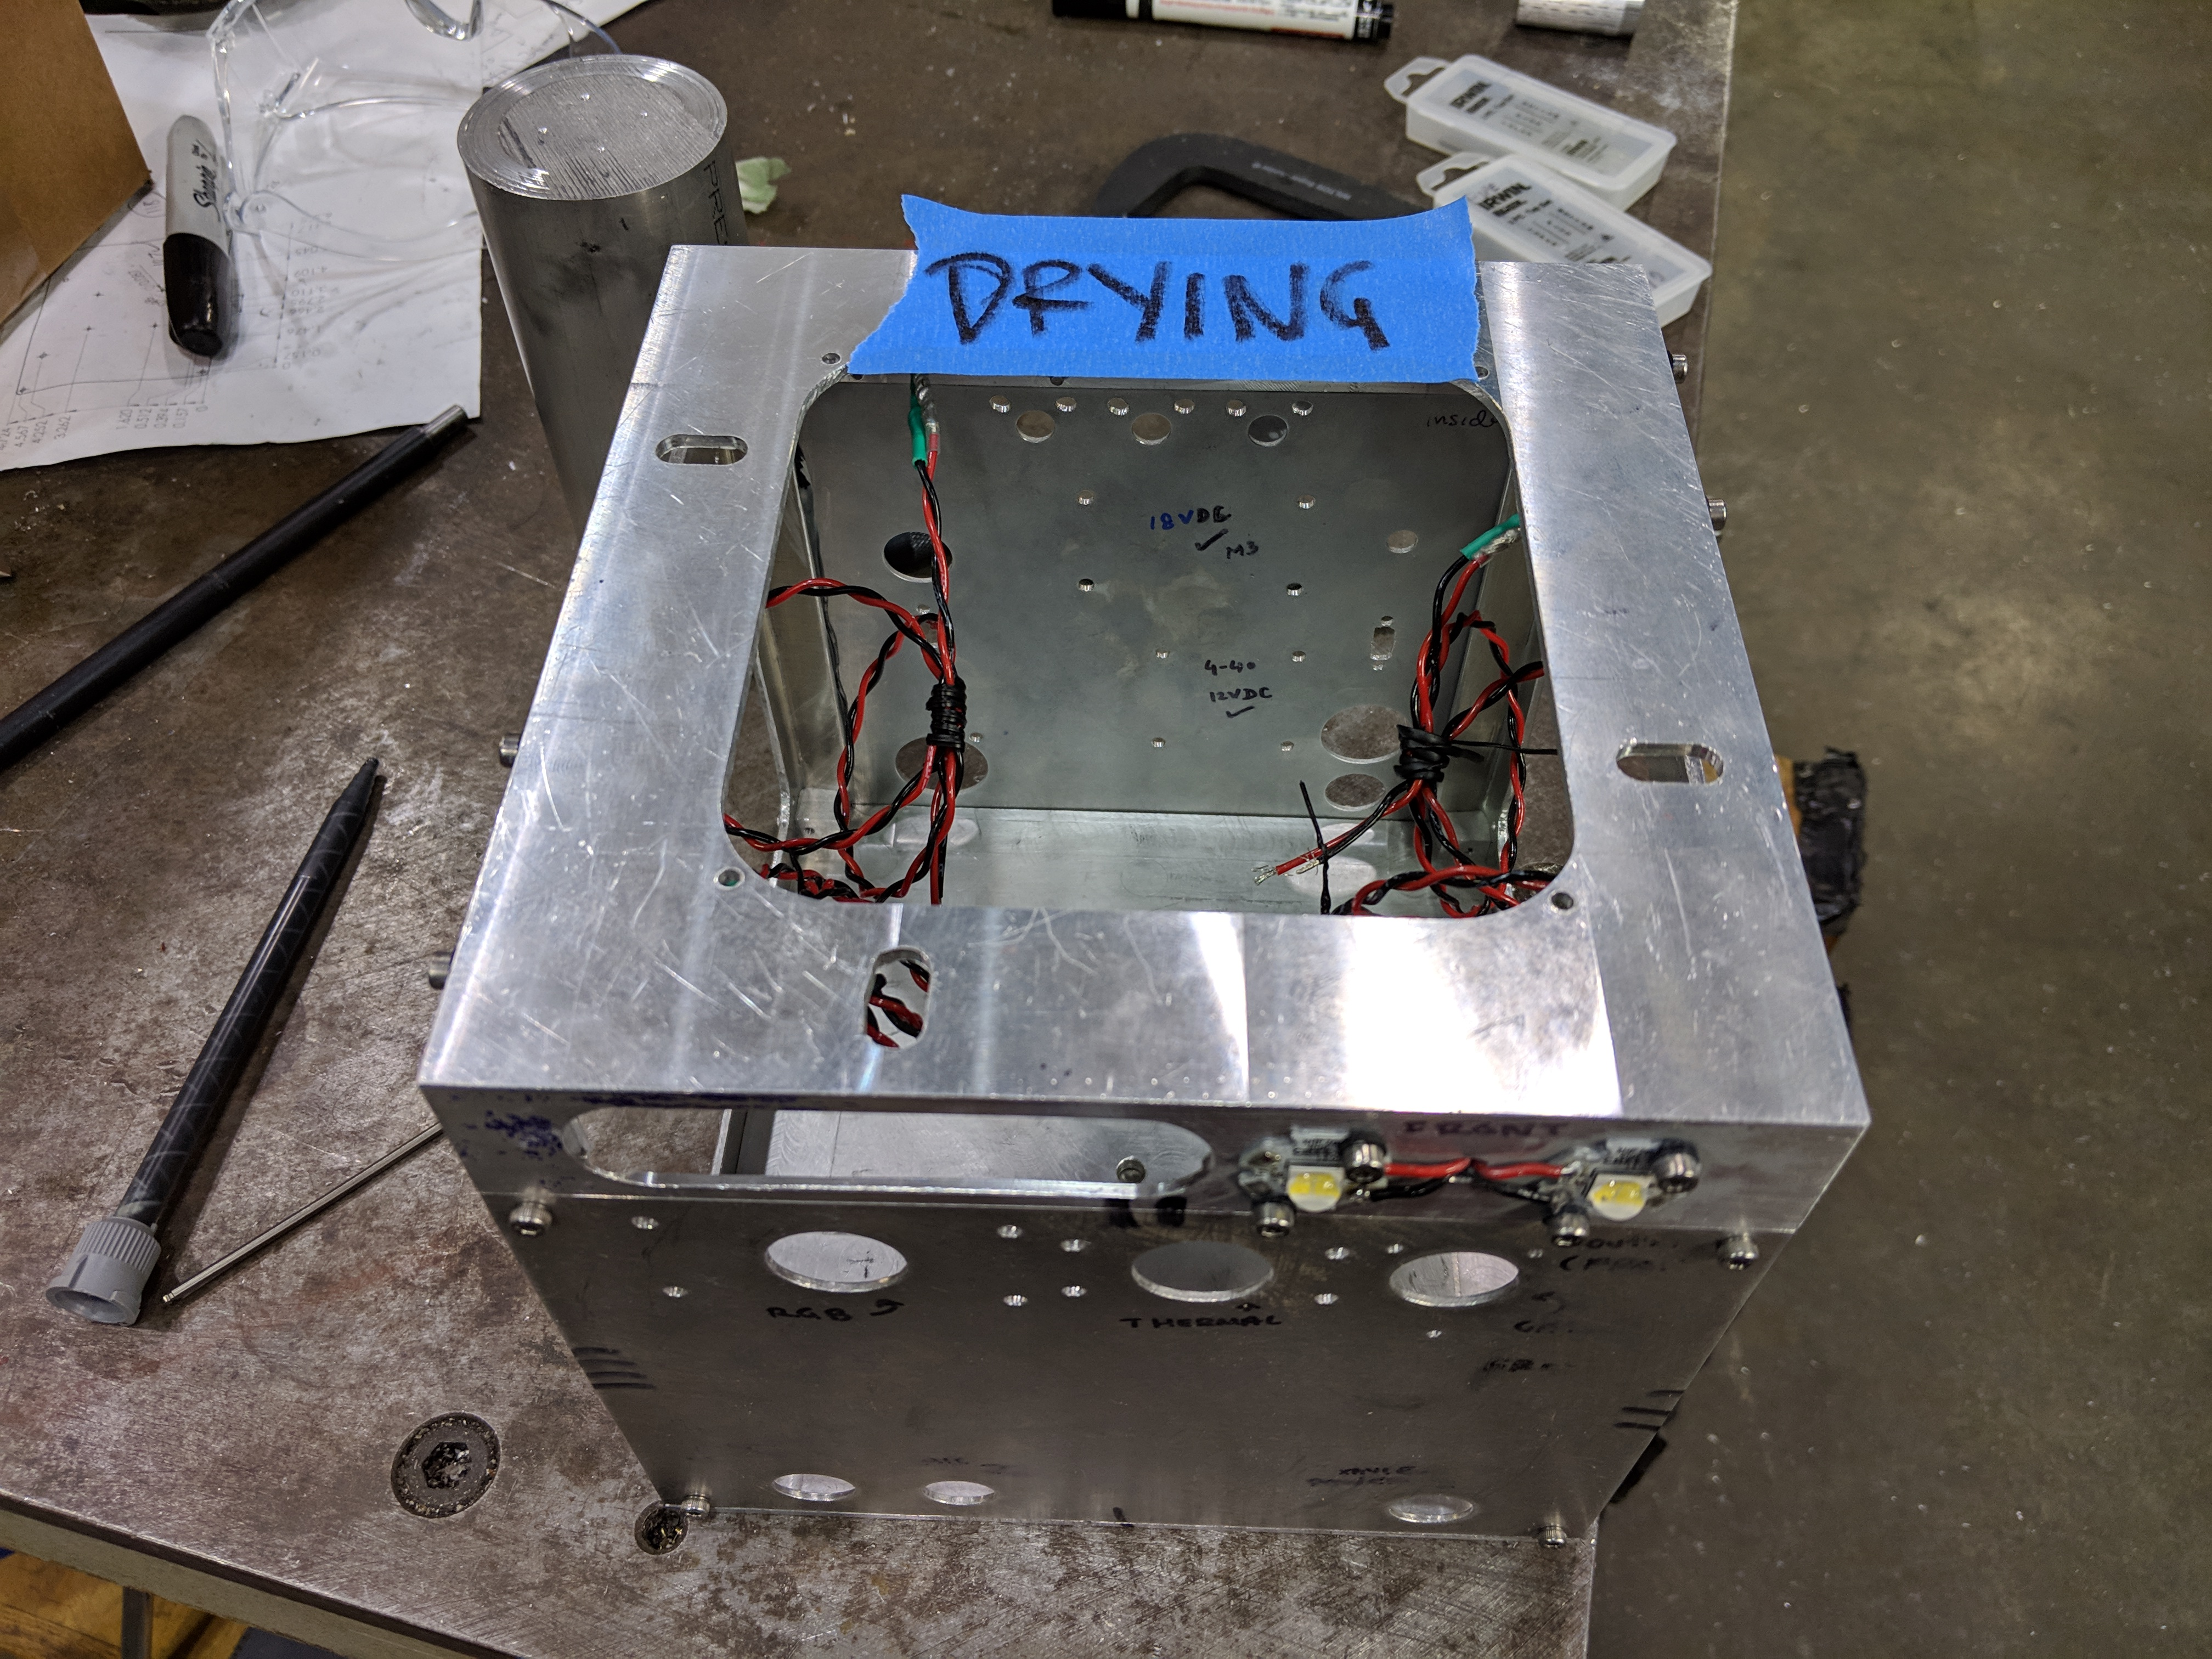
\includegraphics[width=\textwidth]{mk_0/sheet.jpg}
		\caption{Aluminum body panels}
		\label{mk_0_sheet}
	\end{subfigure}		
	\hfill
	\begin{subfigure}{0.32\textwidth}
		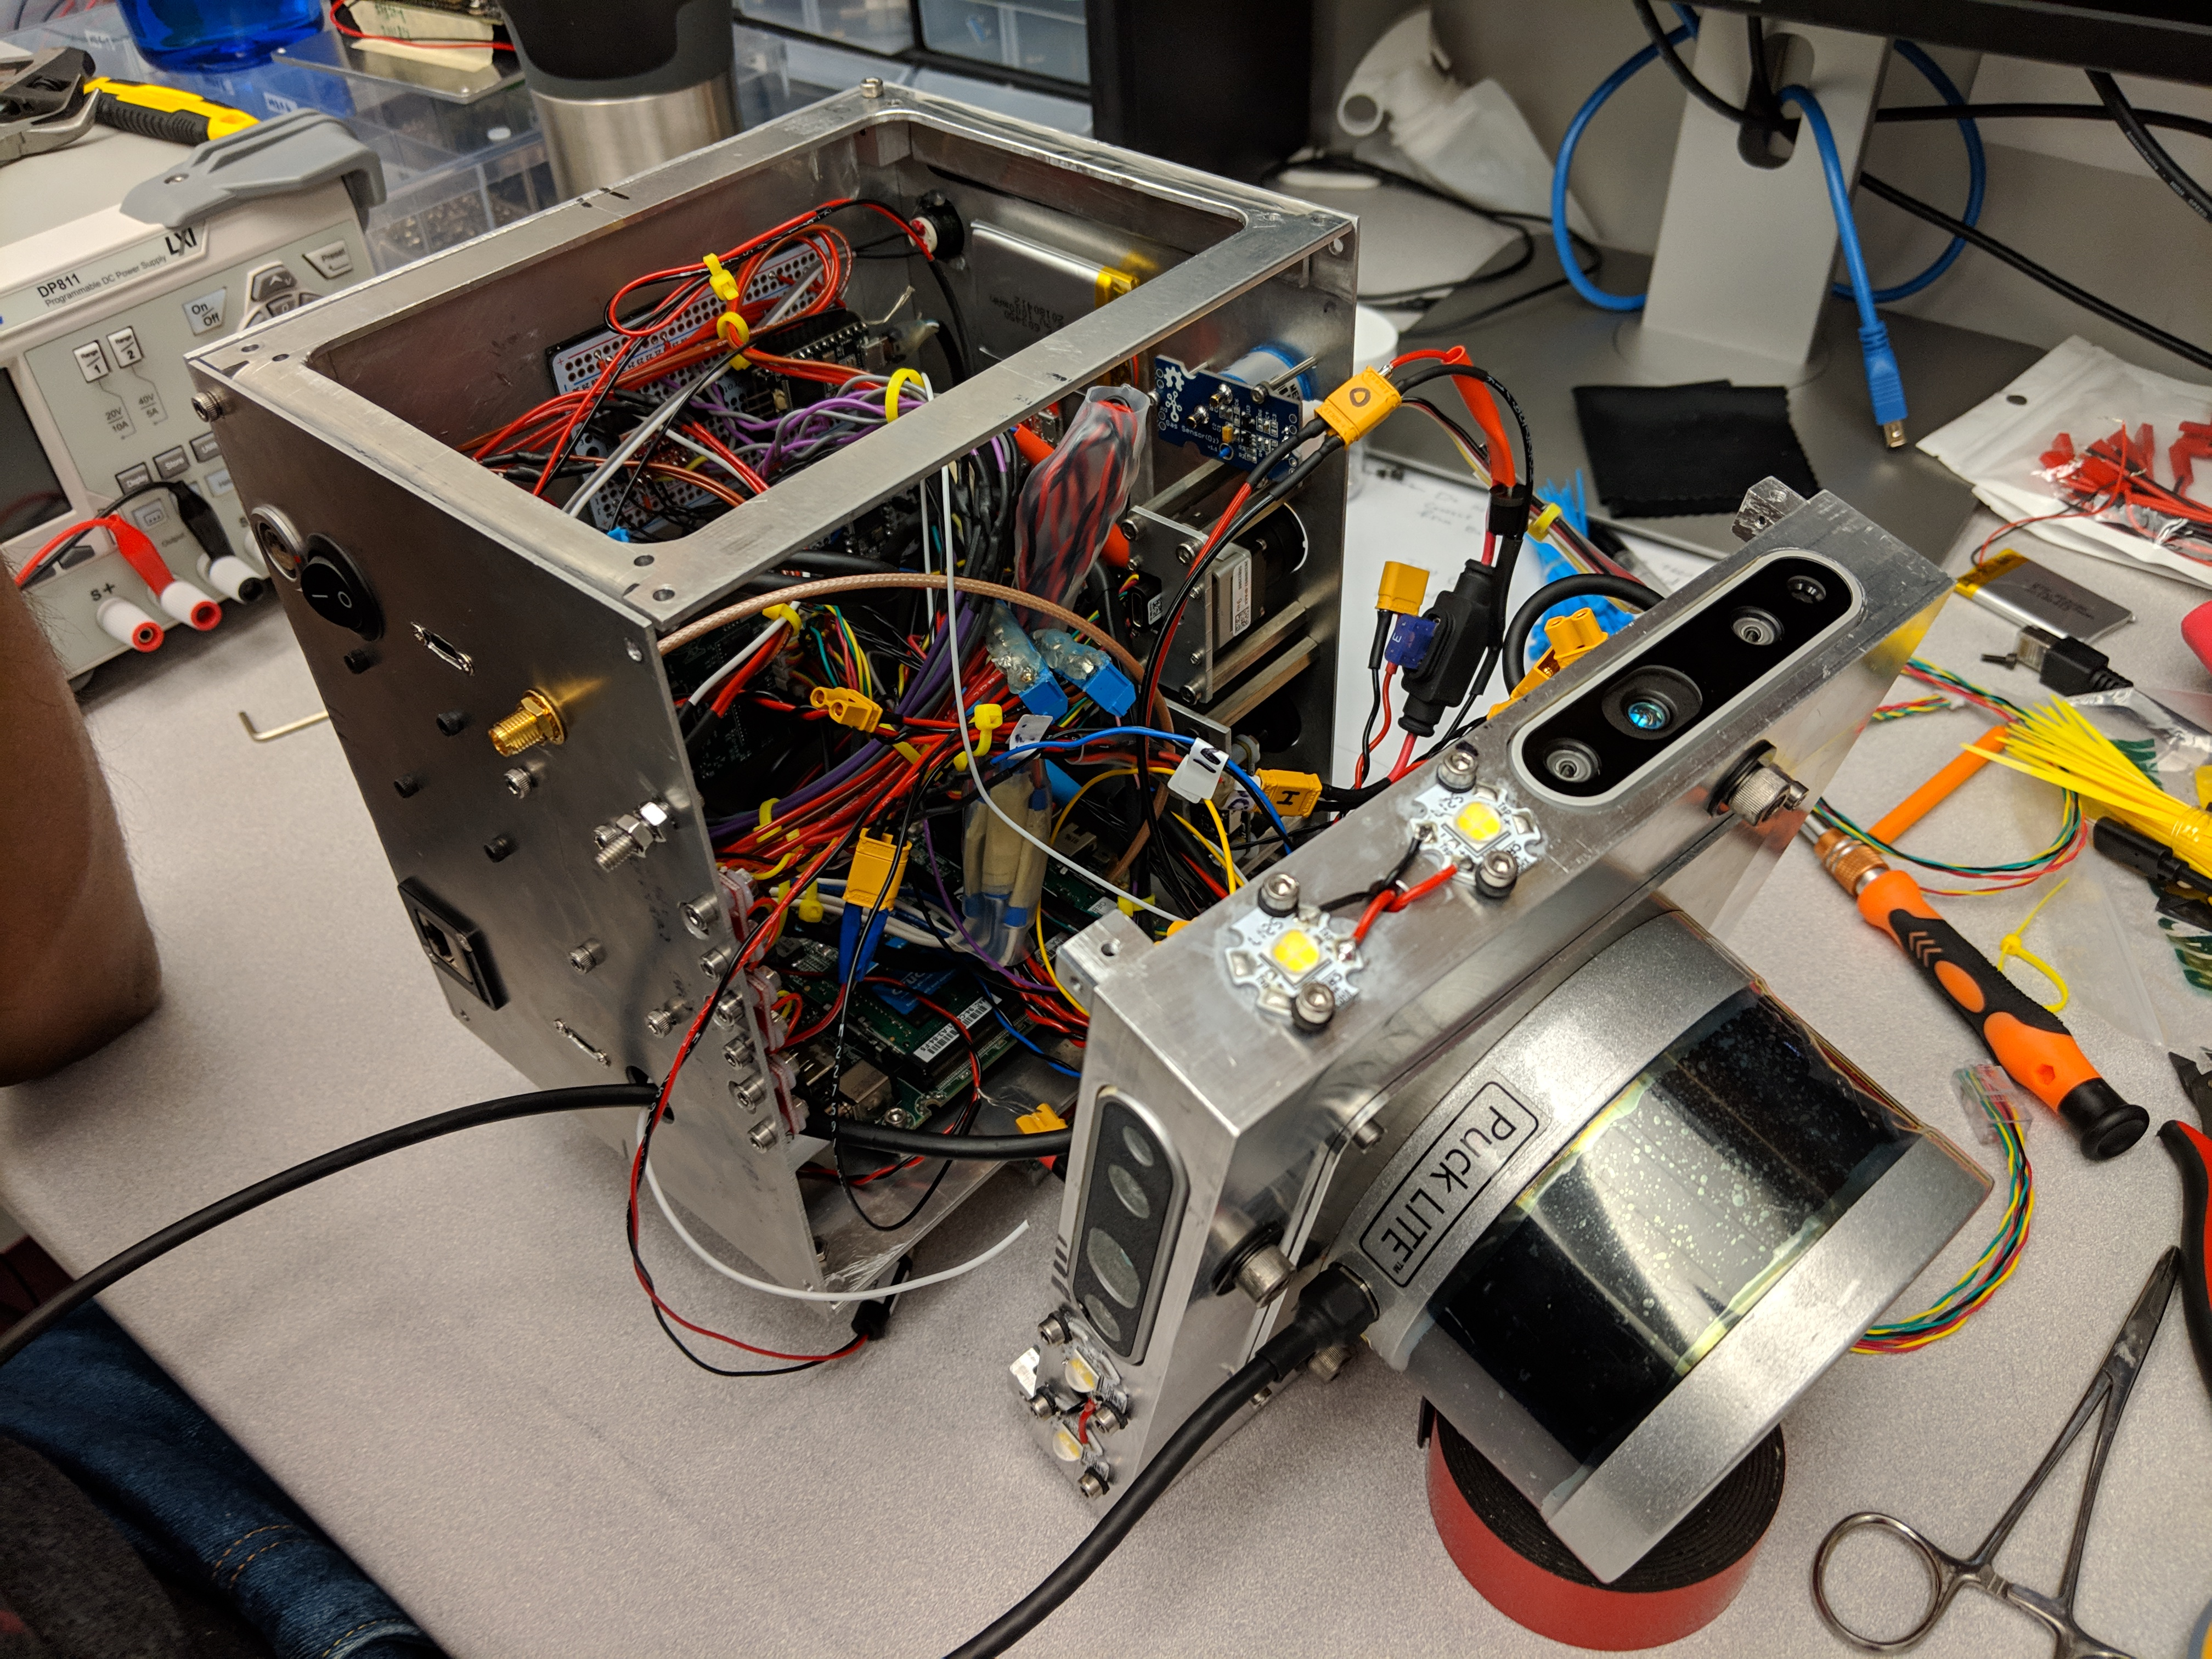
\includegraphics[width=\textwidth]{mk_0/insides.jpg}
		\caption{Initial wiring structure}
		\label{mk_0_wiring}		
	\end{subfigure}
	\hfill
	\begin{subfigure}{0.32\textwidth}
		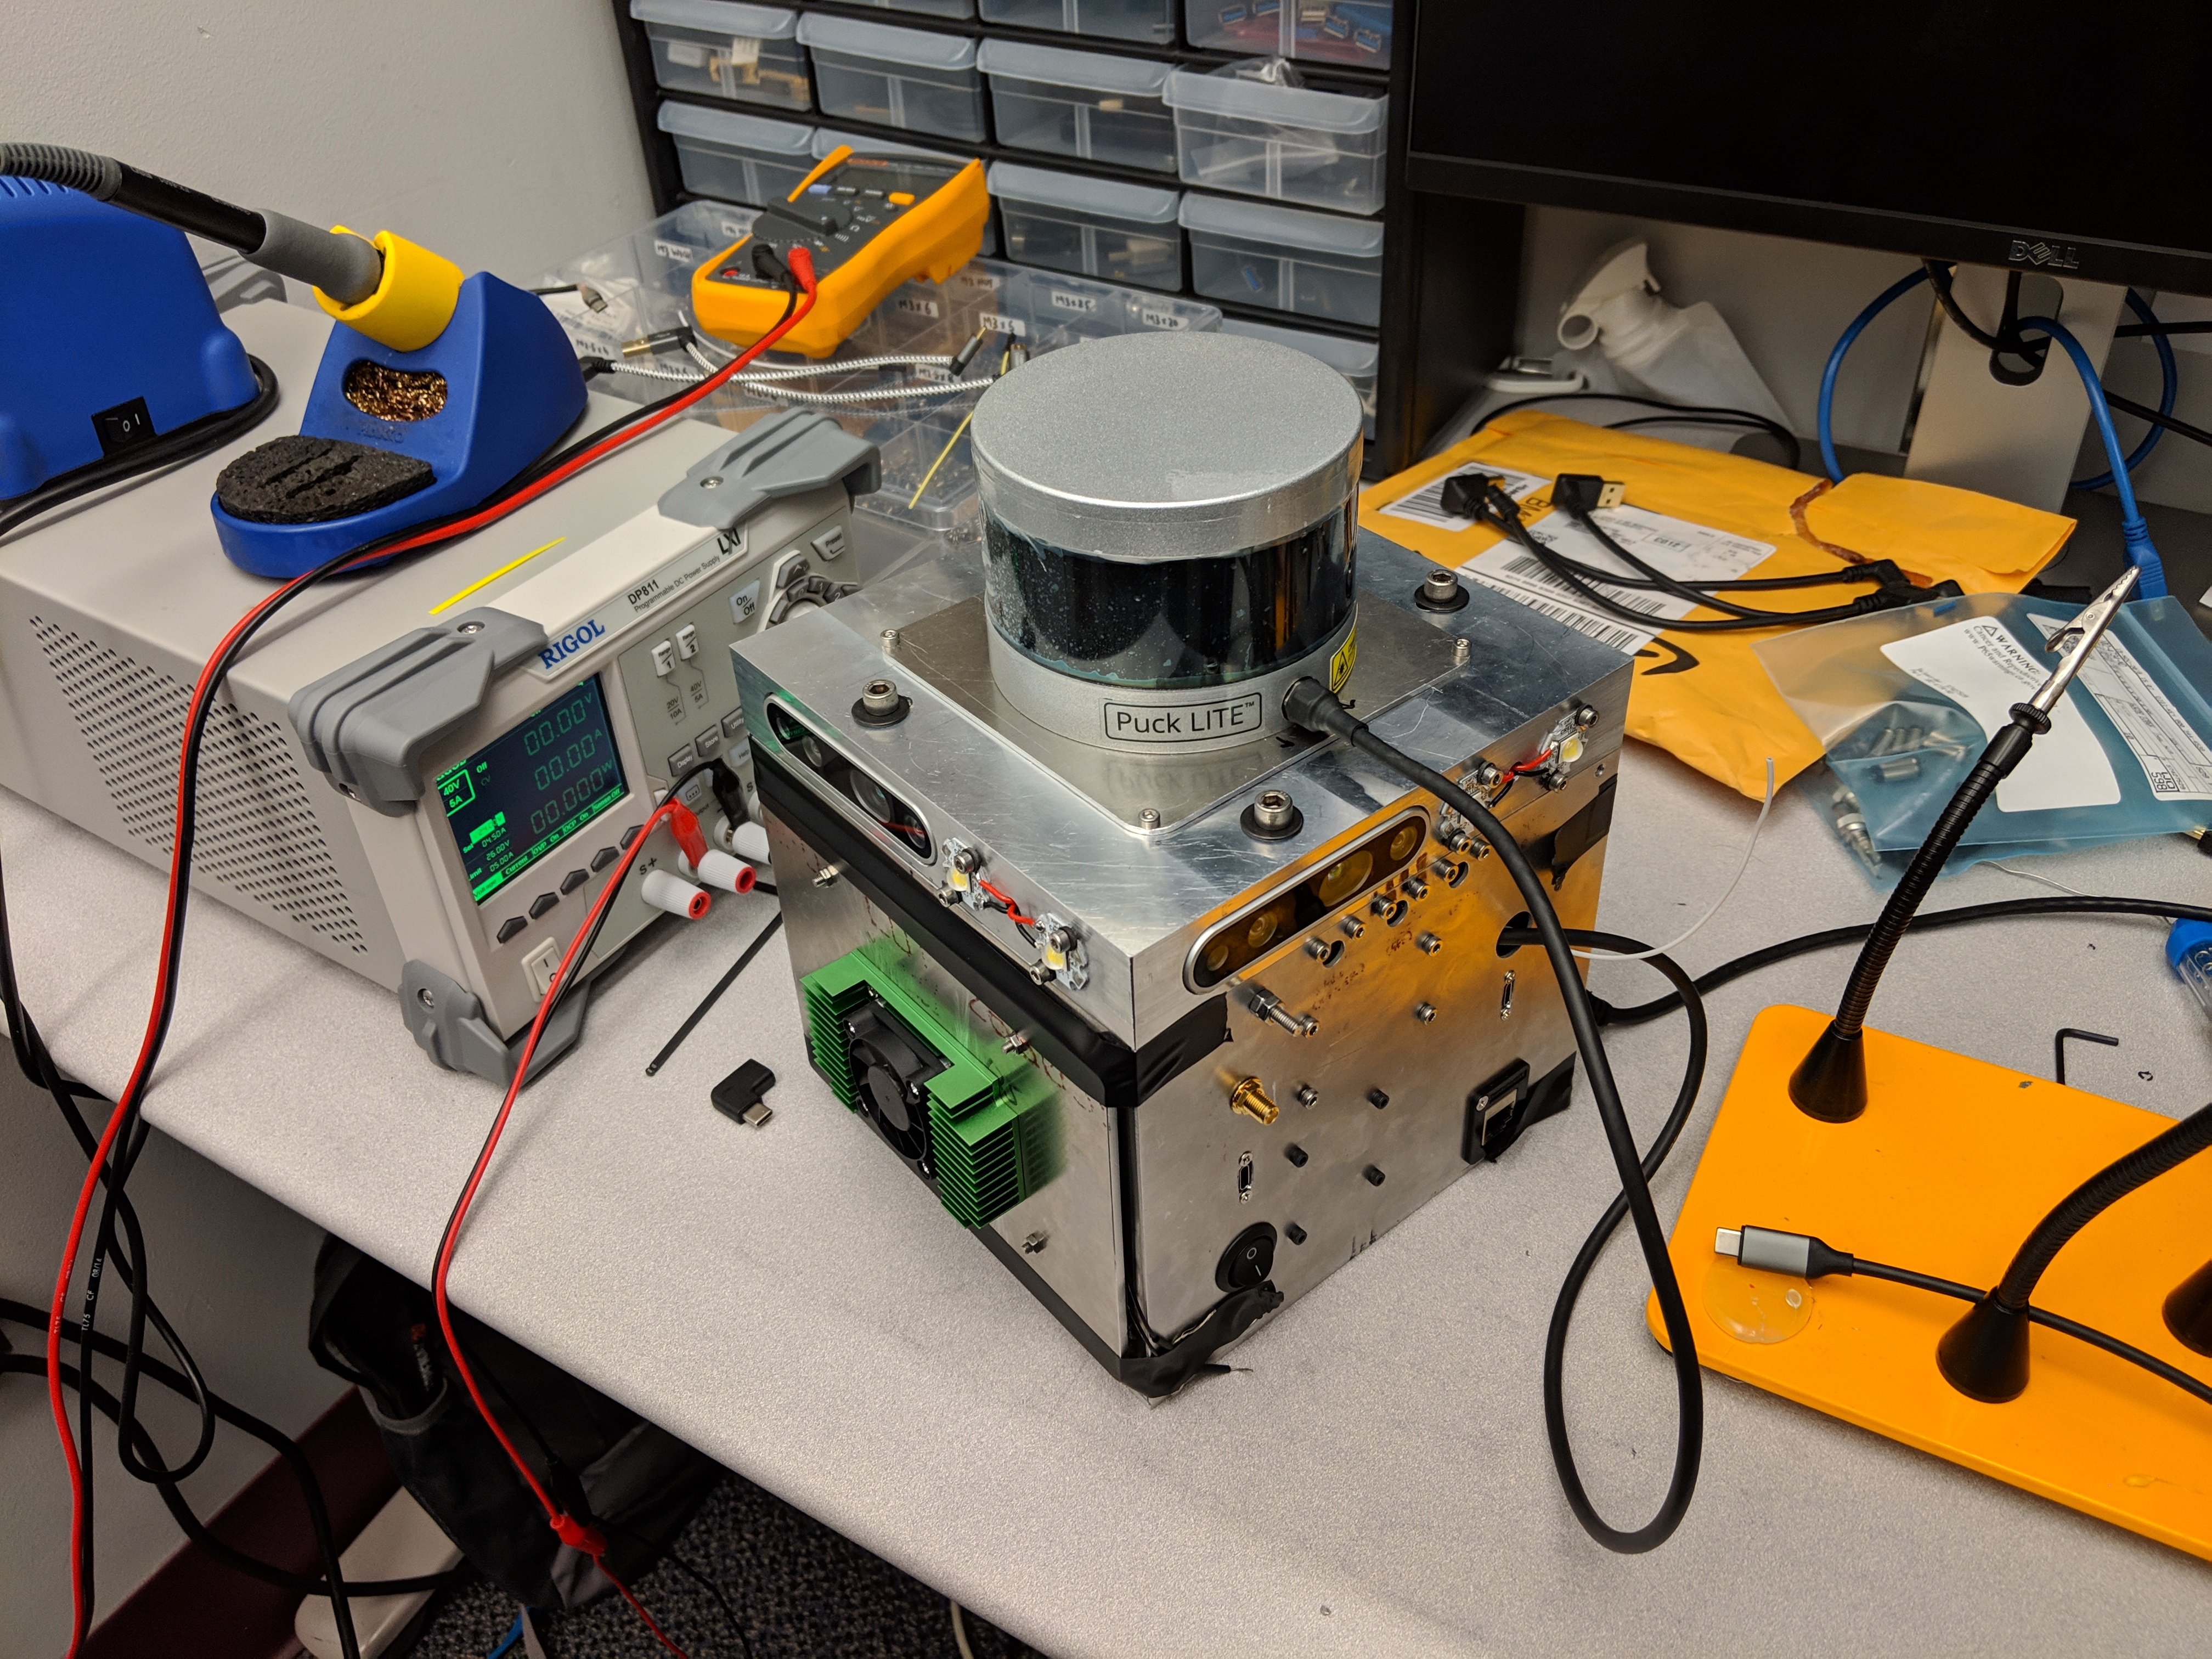
\includegraphics[width=\textwidth]{mk_0/zipped.jpg}
		\caption{Preliminary assembly}
		\label{mk_0_zipped}
	\end{subfigure}	
	\caption[Photos from Mk. 0 initial assembly]{The figure shows various steps from the initial assembly of Mk. 0. The body panels were assembled and adjusted as necessary to ensure a close fit for environmental robustness (HWR3). The electronics were then attached and wired, with enough slack left in the wires to ensure components could be pulled apart for servicing. The initial assembly revealed that everything fit together nicely, but was too large for the drone.}
	\label{mk_0_assembly}
\end{figure}

\section{Drone Payload Development}

The primary constraint for any payload flying on our aerial platforms is weight. Weight is inversely proportional to flight time and dynamics -- a lower weight means improved flight time and better handling under turbulent conditions due to higher thrust to weight ratios. After the first assembly of Mk. 0, it was discovered that the approximately 20 lbs weight of the payload would be too high to fly on D1. A separate, slimmed down version of the payload would be necessary. Reusing existing components on D1, even at the expense of modularity, would be crucial to reducing weight.

Prior to the addition of a payload, D1 already contained sensors and compute necessary for LOAM -- an Intel NUC NUC8i7BEH, a Velodyne VLP 16 LIDAR, and an Xsens IMU. No additional object detection sensors were present. From Table \ref{sensor_utility_categories}, it was clear that the highest utility single sensor would be an RGB camera. The same RGB camera as Mk. 0 was selected for consistency, along with the same lighting solution. Payload weight restrictions prevented adding 4 RGB cameras as was done in Mk. 0. Similarly, weight restrictions prevented adding a separate Nvidia Xavier module to perform object detection, meaning that all object detection code would need to run alongside all other code on the NUC, with adjustments in performance made as necessary to accommodate the resource constraints. The final hardware configuration is pictured in Figure \ref{drone_closeup}.

\section{Mk. 1 Development}

Mk. 0 and the drone payload were initially assembled in early December 2018, in time for the qualification deadline for the DARPA-hosted  SubT Integration Exercise (STIX) event to be held in April 2019. After this deadline, DARPA announced the official list of artifacts which would be used in the Tunnel Circuit (see Figure \ref{tunnel artifacts}) and indicated that the same set of artifacts would be used at STIX. While no modifications were made to the Mk. 0 or Drone Payloads as a result of this new information, this information, along with the experience using Mk. 0 and the Drone Payloads through the STIX event revealed a number of potential areas of improvement for the next ground robot payload, Mk. 1. The improvements made to Mk. 1, as compared to Mk. 0, are outlined in the remainder of this section.

\subsection{RGB Camera Improvements}

The experience at STIX indicated that the most useful category of sensor for detecting the Tunnel Circuit artifacts was RGB cameras. The backpack, drill, fire extinguisher, and survivor artifacts could be easily detected in the RGB camera streams, with cell phones being somewhat more difficult but theoretically possible as well. Thus, the first place attention was directed was improving the quality and usability of the data coming from the RealSense D435 cameras. It was decided early in the development cycle that a new RGB camera would not be used on Mk. 1 due to the rapid timeline requirements (less than 3 months of available development time), as well as to minimize component level differences between the payloads to reduce software complexity.

\subsubsection{Framerate and Resolution}

The most important issue with the RGB cameras on Mk. 0 is the limited framerate and resolution available. Each RealSense D435 module on Mk. 0 streams both RGB (encoded as YUYV) and depth (Z16) at 15 frames per second at a resolution of 640 x 360. The relatively low camera framerate, which allows for long exposure times when using autoexposure, combined with the rolling shutter of the RGB camera frequently causes images to be more blurry than desired. Additionally, the selected resolution is suboptimal for depth accuracy -- a resolution of 848 x 480 is recommended \cite{depthbestpractices}.

The primary restriction on increasing the framerate or the resolution of the RGB images is the available USB bandwidth. In Mk. 0, all 4 RealSense modules are connected to the Xavier via a single USB 3.0 hub (5 Gbps), a HB31C4AB hub from StarTech.com. A variety of framerates and resolutions were tested using the RealSense Viewer application under this configuration prior to the STIX event. Though configurations at both 640 x 360 at 30 fps per camera (885 Mbps) and 848 x 480 at 15 fps per camera (782 Mbps) both appeared mostly stable, frames would be reported as dropped infrequently. The highest framerate and resolution configuration under which no frame drops were observed is 15 fps at 640 x 360 per camera, and thus this configuration is used on Mk. 0. The results reported by Intel \cite{depthmulticam} indicate that these configurations should both be well under the USB bandwidth after which frame drops occur. The discrepancy may be due to different cabling, a different USB hub, or a different scheduling algorithm in the USB host controller used on the Xavier. 

The solution for Mk. 1 was to split the RealSense depth modules over two separate USB ports, each of which has its own host controller on the Xavier. This increases the maximum theoretical bandwidth available from 5 Gbps to 10 Gbps, as well as decreases the number of devices per bus to 2, decreasing bus contention for each host controller and making the scheduling problem slightly easier. This solution was implemented by using a second HB31C4AB hub attached to the second USB Type C port on the developer kit carrier board. Under this new configuration, 30 fps at 848 x 480 resolution (1563 Mbps) was achieved on both the depth and RGB streams for all 4 RealSense modules, as desired. However, it was discovered that the increased data rate filled up the onboard storage too quickly, and thus an identical configuration to Mk. 0 is used on Mk. 1 until more onboard storage can be added.

\subsubsection{Mounting}

The RealSense cameras in Mk. 0 are mounted to the payload using the single $\frac{1}{4}$-20 threaded hole on the bottom, to which a bolt is attached through a slot in the top of the payload. This slot allows for some translational motion of the cameras, while the single attachment point allows the cameras to rotate. Both problems were addressed to some extent with locking washers, but they did not completely eliminate the problems. As the cameras deviate from their calibrated positions, accuracy of downstream algorithms suffers. Thus, the RealSense modules in Mk. 1 are mounted using the 2 mounting points on the back of the RealSense to multiple attachment points on the payload, eliminating the possibility of any motion.

\subsubsection{Orientation}

An additional consequence of the mounting mechanism for the RealSense cameras on Mk. 0 is that all images appear to be upside down. This is compensated for in the software running on Mk. 0, but has a slightly computational cost and requires additional bookkeeping. To eliminate the additional CPU burden, the mounting mechanism on Mk. 1 ensures that the cameras are oriented normally.

\subsubsection{Occlusion}

The back RealSense camera module on Mk. 0 has its field of view partially occluded by the communication node droppers on both R1 and R2. If the possibility of placing an aerial vehicle such as D1 on the back of R1 or R2 were explored, the back camera's field of view would be further obstructed. For Mk. 1, this problem is solved by orienting the back camera upwards slightly so that it no longer sees any part of the ground robot. Having a camera oriented slightly upwards also allows the Mk. 1 payload to detect artifacts which may be on high shelves which were previously out of the field of view of the other cameras, at the cost of some redundancy in field of view. An example of the occlusion on Mk. 0 and tilted orientation on Mk. 1 is shown in Figure \ref{mk_1_rear_tilt}.

\begin{figure}
	\centering
	\begin{subfigure}{0.32\textwidth}
		\centering
		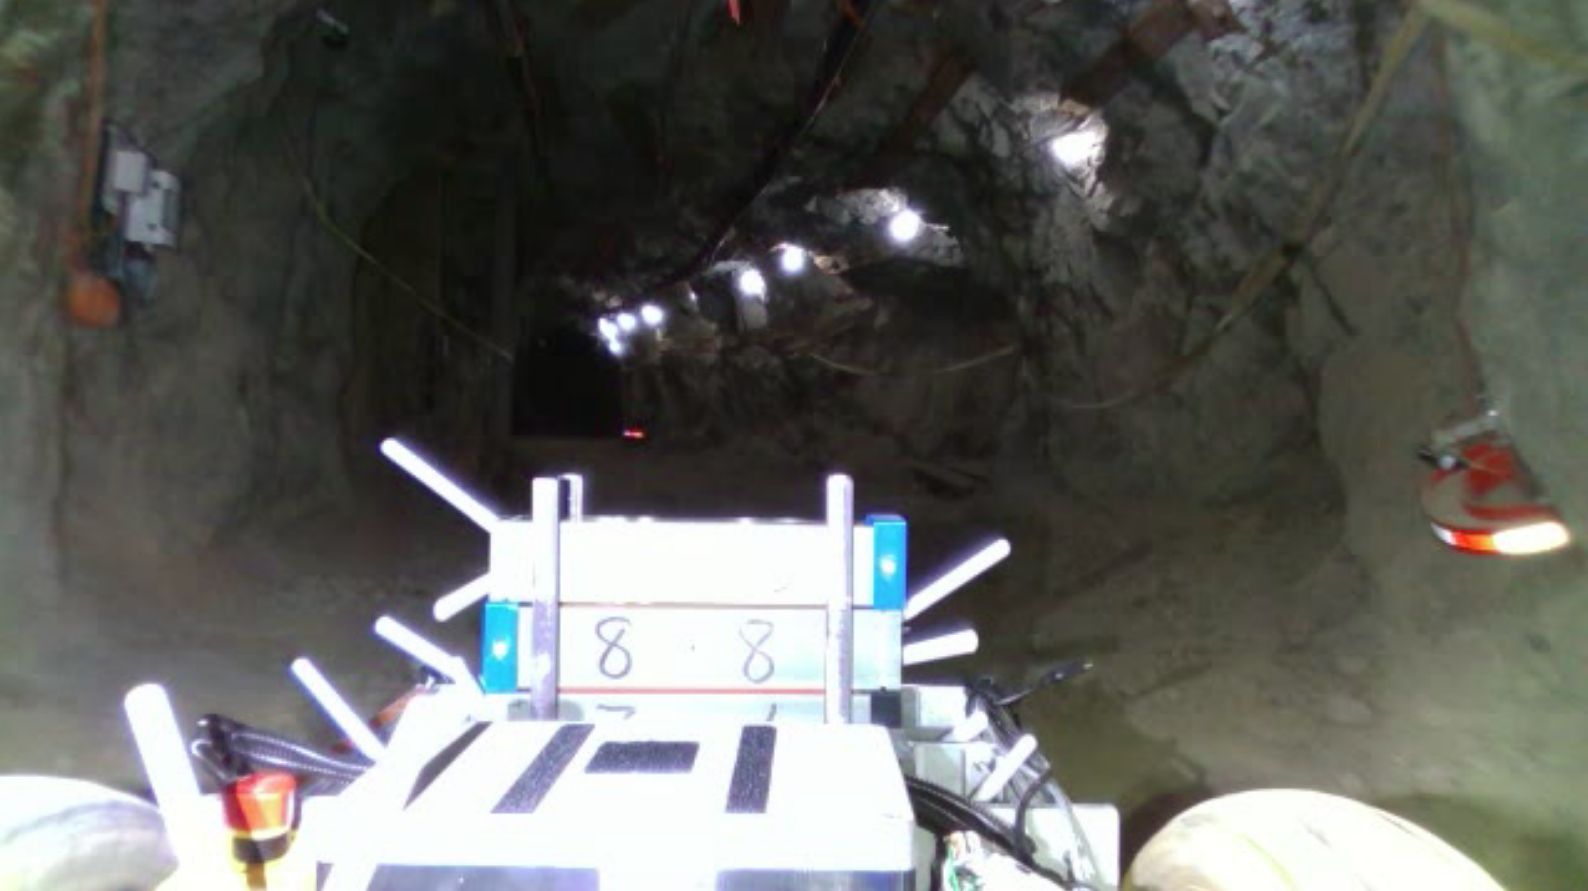
\includegraphics[width=\textwidth,height=3.5cm,keepaspectratio]{rear_occlusion.png}
		\caption{Mk. 0 Self-occlusion}
		\label{rear_occlusion}
	\end{subfigure}
	\hfill
	\begin{subfigure}{0.32\textwidth}
		\centering
		\includegraphics[width=\textwidth,height=3.5cm,keepaspectratio]{mk_1_rear_side.jpg}
		\caption{Mk. 1 back camera tilt}
		\label{mk_1_rear_side}
	\end{subfigure}		
	\hfill
	\begin{subfigure}{0.32\textwidth}
		\centering
		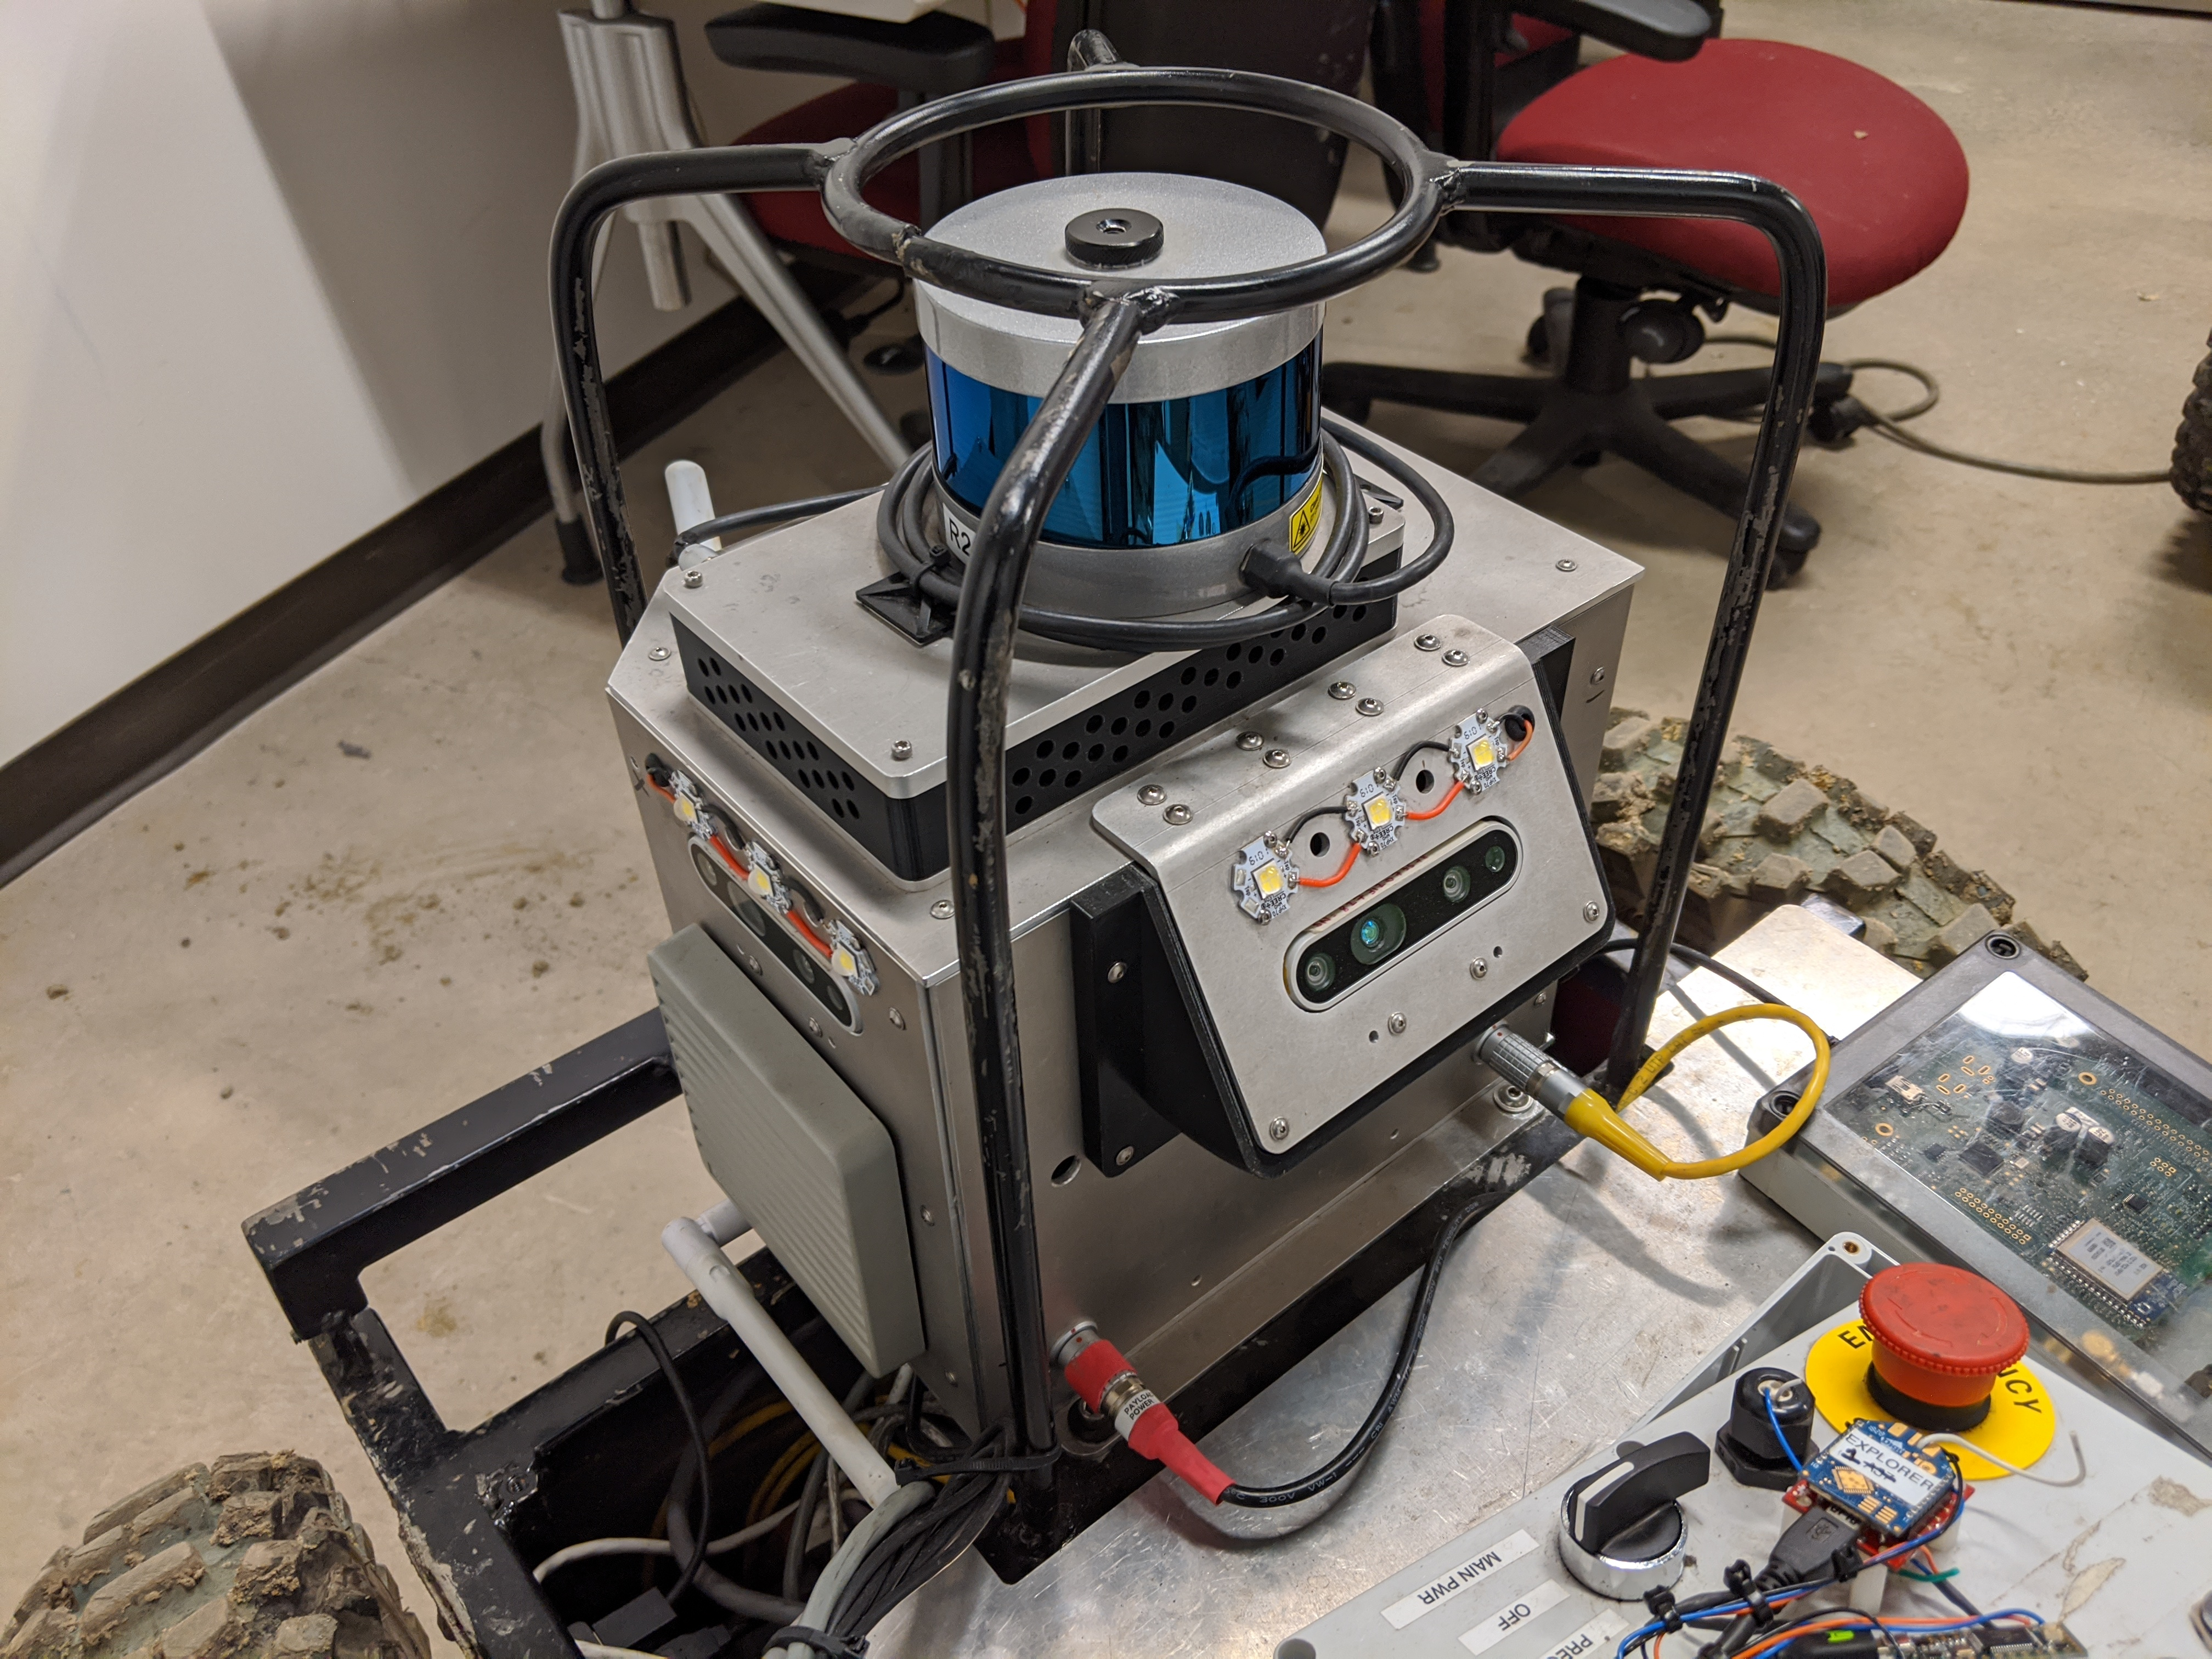
\includegraphics[width=\textwidth,height=3.5cm,keepaspectratio]{mk_1_rear.jpg}
		\caption{Mk. 1 back camera tilt}
		\label{mk_1_rear}
	\end{subfigure}	
	\caption[Tilting back RGB camera on Mk. 1]{The back RealSense module on Mk. 1 is tilted to avoid the self occlusion problems of Mk. 0. The tilt also allows for previously unseen views to be captured by the rear camera, making it possible to detect artifacts on or near the ceiling.}
	\label{mk_1_rear_tilt}
\end{figure}

\subsection{Thermal Camera Improvements}

The thermal camera on Mk. 0 offers a relatively low native resolution and framerate of 320 x 256 and 8.5 Hz respectively. The low framerate is due to a limitation of the specific camera model selected -- a higher framerate version is not readily available. Additionally, with only a single thermal camera, the overall field of view is relatively limited. Artifacts to either side of the robot are often missed, or only captured for a single frame or two by the single front-facing thermal camera on Mk. 0. Finally, there is a consistent dark spot in the center of the thermal images captured from Mk. 0, as well as on those captured from spares, shown in Figure \ref{mk_0_dark_center}. Conversations with FLIR indicated that this may be caused by the camera self-heating over time, as well as perhaps a bad lens calibration, bad sensor, or bad flat field correction, though no specific cause was determined.

\begin{figure}
	\centering
	\begin{subfigure}{0.32\textwidth}
		\centering
		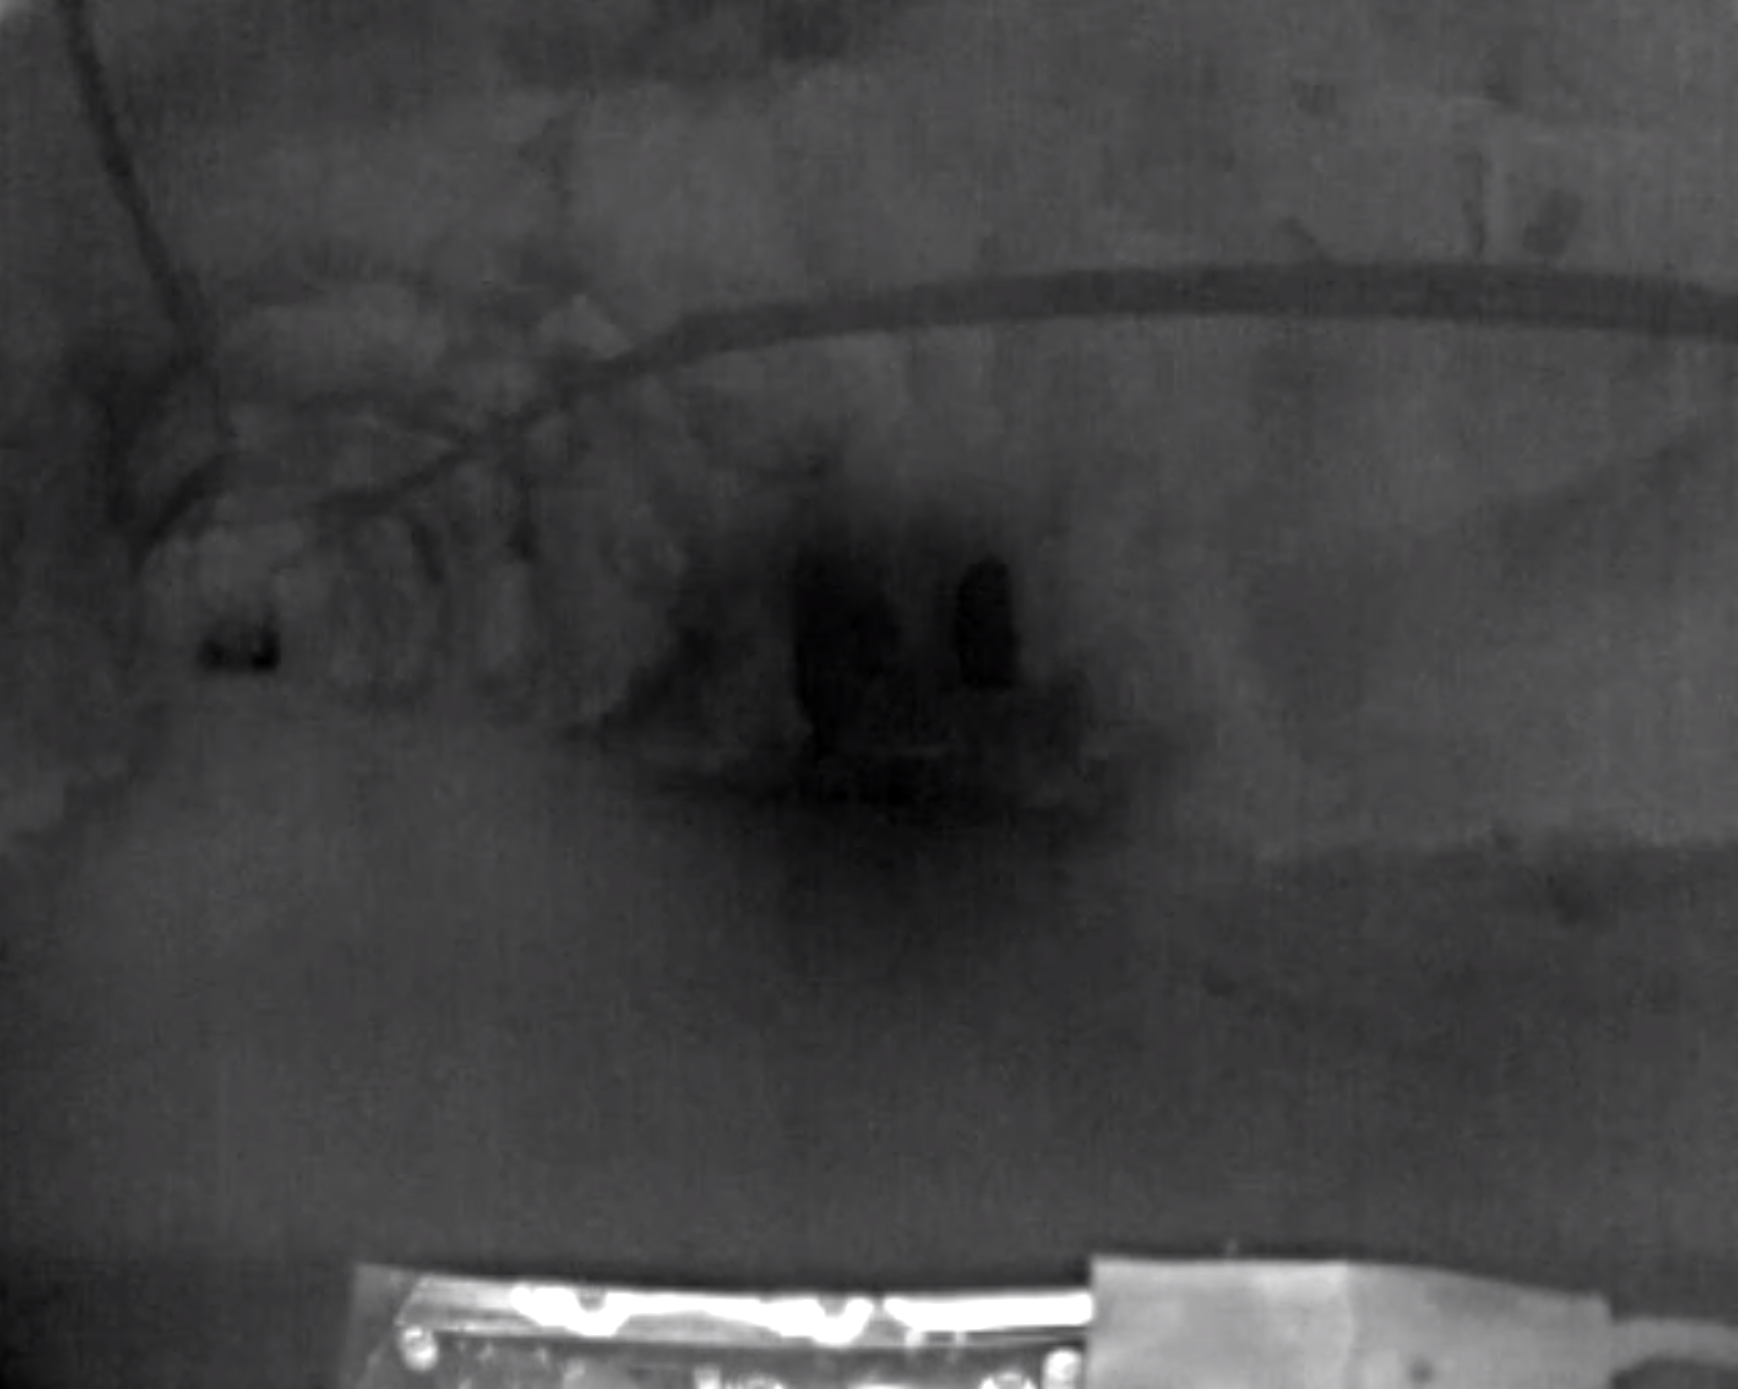
\includegraphics[width=\textwidth]{dark_1.png}
		\label{dark_1}
	\end{subfigure}
	\hfill
	\begin{subfigure}{0.32\textwidth}
		\centering
		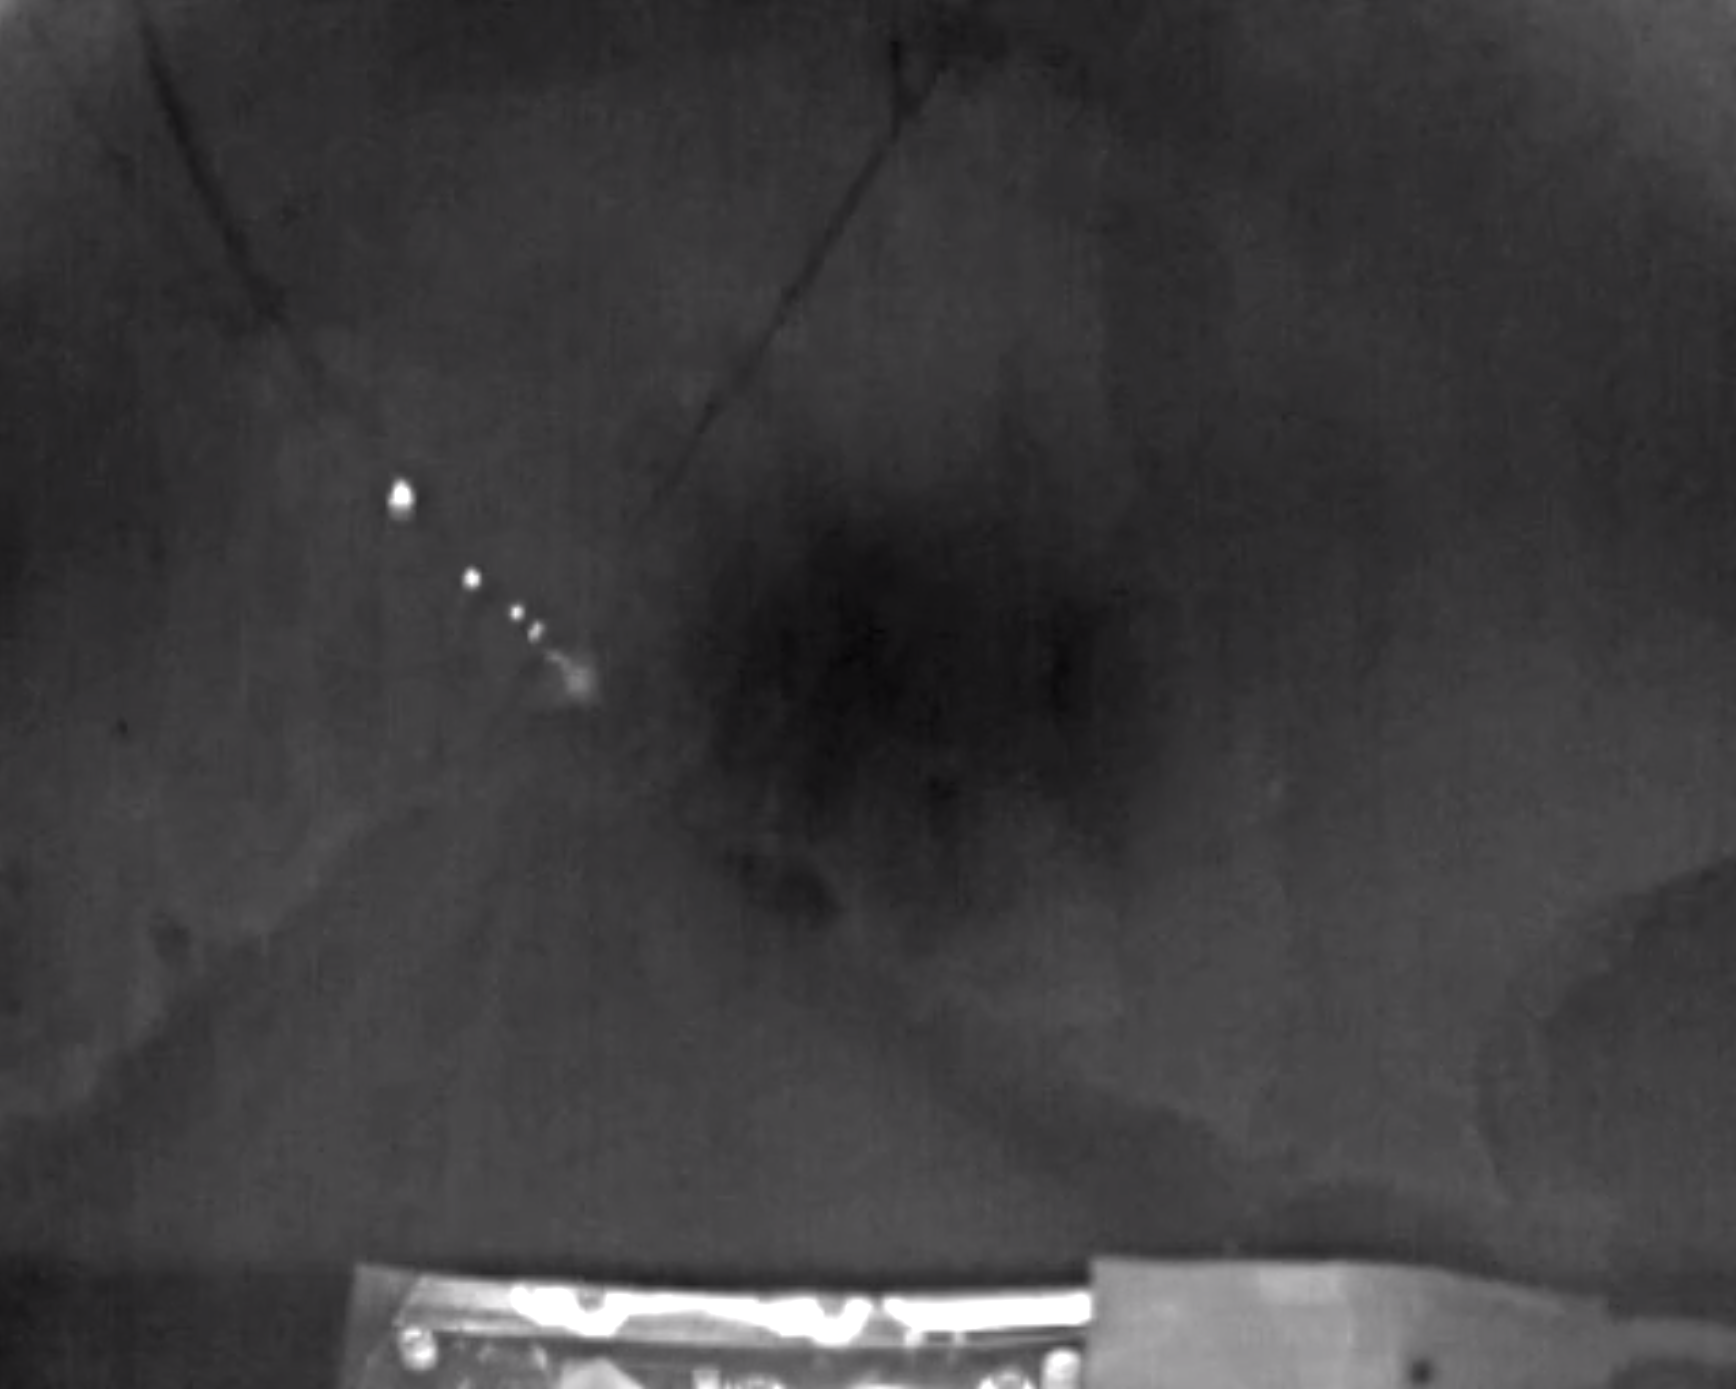
\includegraphics[width=\textwidth]{dark_2.png}
		\label{dark_2}
	\end{subfigure}		
	\hfill
	\begin{subfigure}{0.32\textwidth}
		\centering
		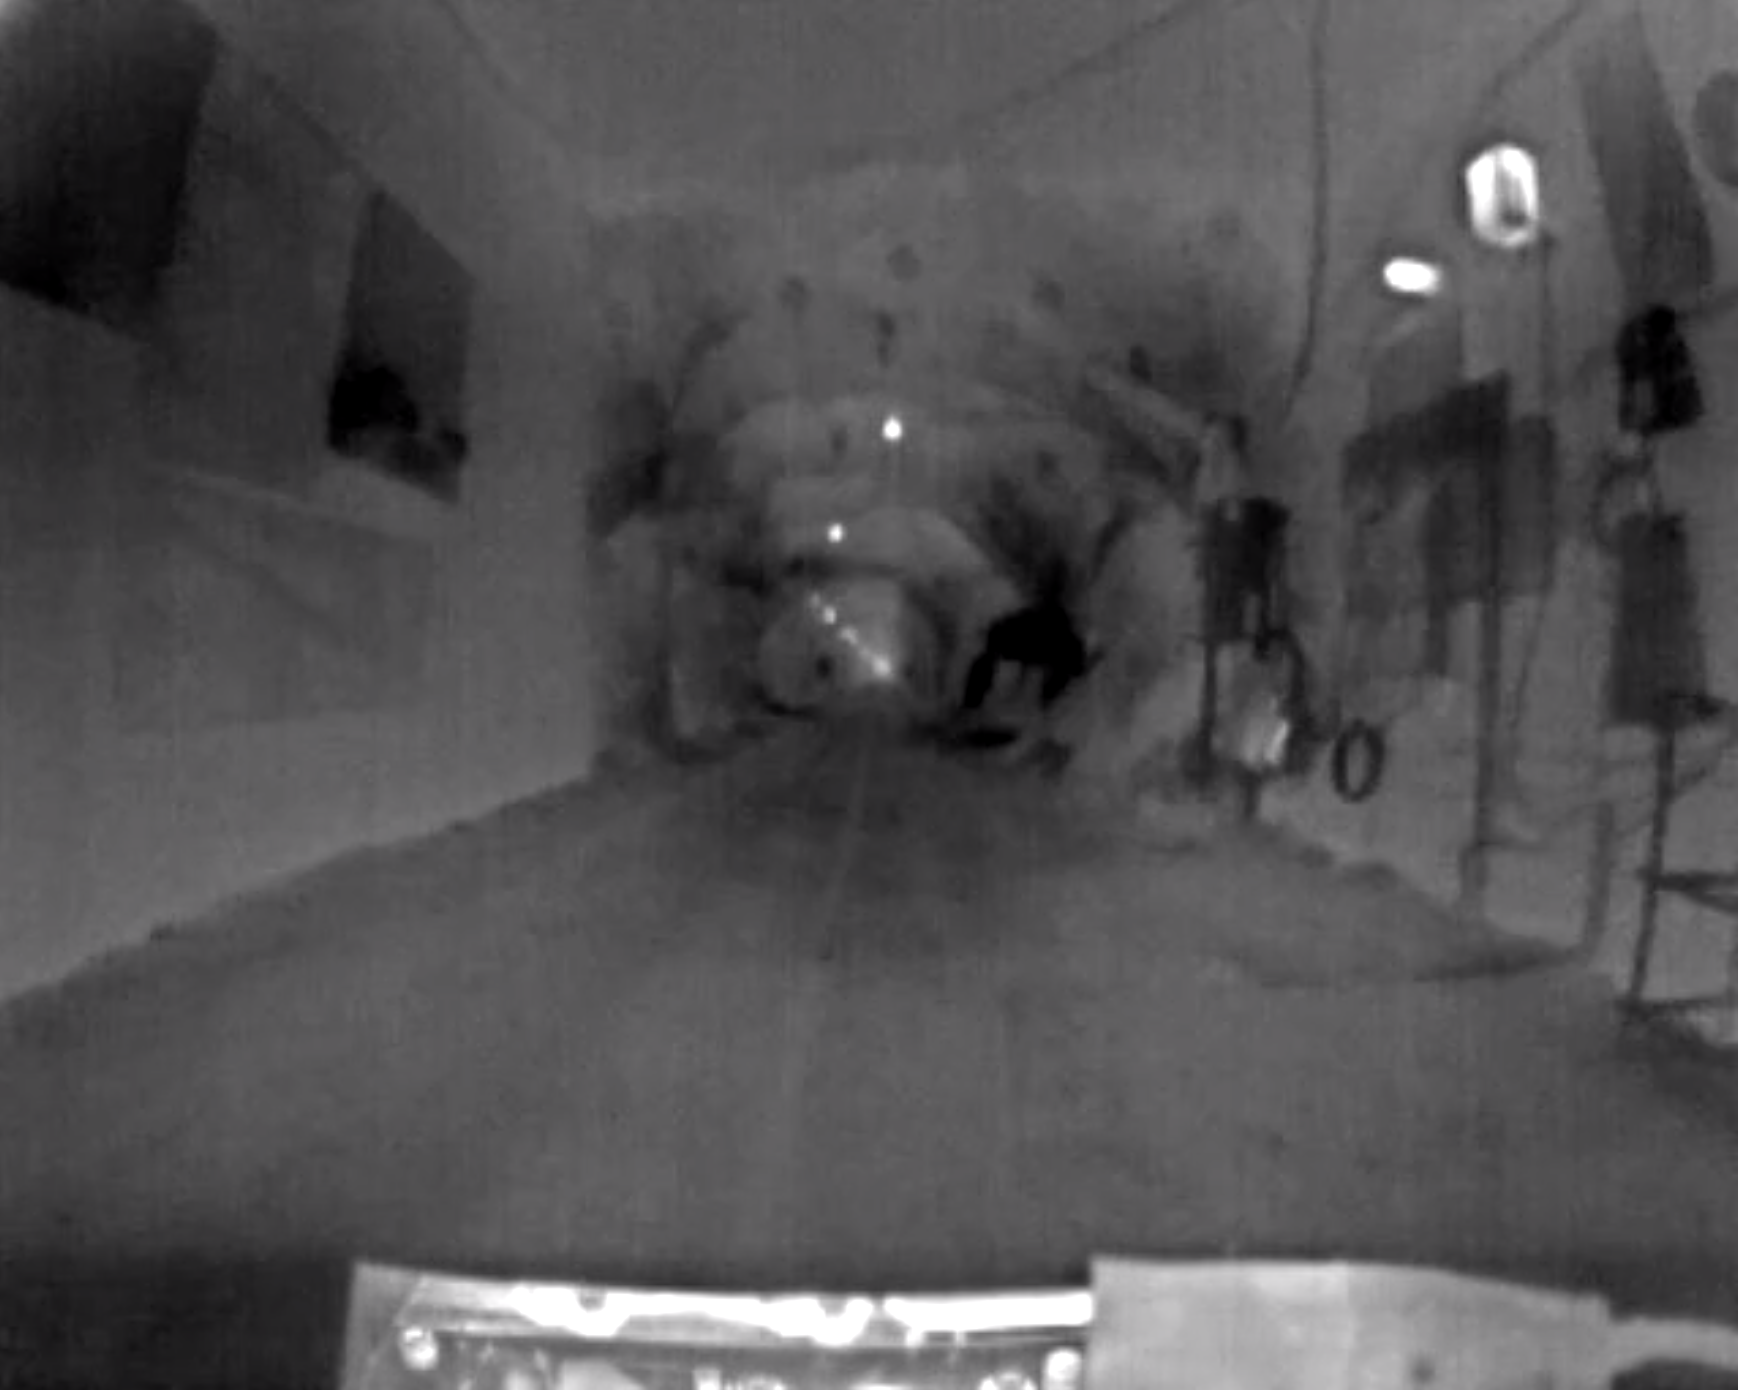
\includegraphics[width=\textwidth]{dark_3.png}
		\label{dark_3}
	\end{subfigure}	
	\caption[Dark spot visible on Mk. 0 thermal camera]{The center of each of the 3 images captured from Mk. 0's thermal camera shows an unexpected dark spot. This dark spot is present on images captured from the spares of the same camera model as well, but is not present on the new thermal cameras selected for use in Mk. 1.}
	\label{mk_0_dark_center}
\end{figure}

To resolve all of these issues for Mk. 1, 2x FLIR Boson 640, a higher end sibling of the FLIR Boson 320 used on Mk. 0, were selected. This new thermal camera offers framerates of 30 and 60 fps at a native resolution of 640 x 512, and uses a different lens assembly which offers a 95 degree HFOV. The dark center spot observed in Mk. 0's thermal camera is not observed in the Mk. 1 thermal cameras. The two cameras are positioned at the front diagonal corners of Mk. 1, covering the front 185 degrees of field of view.

Unfortunately, the interface for the new thermal cameras is USB 2.0, the same as the interface for the thermal cameras in Mk. 0. While the maximum available bandwidth over USB 2.0 is sufficient to stream 1 of the FLIR Boson 640s at 60 fps (YV12 encoding, 236 Mbps), we were unable to achieve sustained 60 fps streaming on two cameras on the the same USB port. This would require 472 Mbps of throughput over USB 2.0 which, while under the theoretical maximum bitrate, is higher than any practical implementation achieves due to transmission overhead and scheduling inefficiencies. Luckily, the changes to the RGB cameras for Mk. 1 included the addition of a second USB hub, which allows the 2 new thermal cameras to operate on separate USB 2.0 ports. The maximum framerates observed on the RealSenses on Mk. 1 were not affected as a result of this change.

\subsection{Illumination Improvements}

A few problems with the illumination system were observed when working with Mk. 0:

\begin{description}
	\item[Flickering] The Mk. 0 LEDs constantly flicker. This flickering is fast enough that it is not visible in the camera images, but is sufficiently distracting for humans working with and around the robot that it needed to be fixed for Mk. 1.
	\item[Switch control] The Mk. 0 LEDs are controlled by a physical switch on the payload. Part of the operational procedure for deployments is to ensure that the LEDs have been switched on. However, this step occasionally gets missed, and has resulted in deployments (including once at STIX) without the LEDs activated, limiting the effectiveness of the RGB cameras. For Mk. 1, the LEDs needed to be controlled automatically.
	\item[Fixed brightness] A byproduct of powering all of the LEDs on Mk. 0 with a single 12V regulator is that the brightness cannot be adjusted (beyond the unintended flickering). While brightness control is not strictly necessary for basic operation, it could serve as a way to manage power consumption and heat production and was a requested feature for Mk. 1 as well.
\end{description}

The first attempt at solving all 3 of these problems was to use a custom PCB to drive the LEDs. Each PCB drives LEDs using the same voltage regulation strategy as in Mk. 0, though with a higher quality regulator intended to reduce flicker. The PCBs also contain a programmable microcontroller which allows another computer, such as the Xavier, to control the brightness of the LEDs by issuing commands over I2C. The PCB has an input for the depth trigger produced by the RealSense depth modules (see Figure \ref{realsense_scope}) which can be used to automatically turn on the LEDs, as the trigger is only produced when the camera is broadcasting images. Early results indicated that the PCBs would be able to solve all of the problems with illumination from  Mk. 0. The PCB is shown in Figure \ref{led_board}.

Unfortunately, while the PCBs were being developed, it was decided that a third LED should be used per side to provide additional illumination, to compensate for the reduced exposure time at the new maximum framerate of 30 fps for RGB images. The current requirements for the third LED proved to be too high for the PCB, which was only designed with the current of 2 LEDs in mind. By the time this issue was discovered, it was too late to upgrade the voltage regulator and fabricate new PCBs. While some of the manufactured PCBs were able to handle the current for 3 LEDs, not all boards were able to do so reliably, which meant that the boards could not be used in a field deployment. The fallback plan, which was implemented for Mk. 1, was to use the BuckBlock A009 LED drivers which had been used for prototyping and the earlier LED flashing experiments.

The BuckBlock drivers solve the flicker problem by providing a constant current source rather than a constant voltage source. They do not offer a programmatic way to control LED brightness, but do support the use of a potentiometer to control brightness manually. The BuckBlocks used in Mk. 1 are also wired directly into power, rather than through a switch, and turn the LEDs on whenever power is applied to the payload. This is a less optimal solution than turning on the LEDs automatically with the image streaming as the PCBs would have been able to do, but it solves the primary problem of forgetting to turn the lights on. We intend to continue development on the custom PCB for use in future iterations of the payload.

\begin{figure}
	\centering
	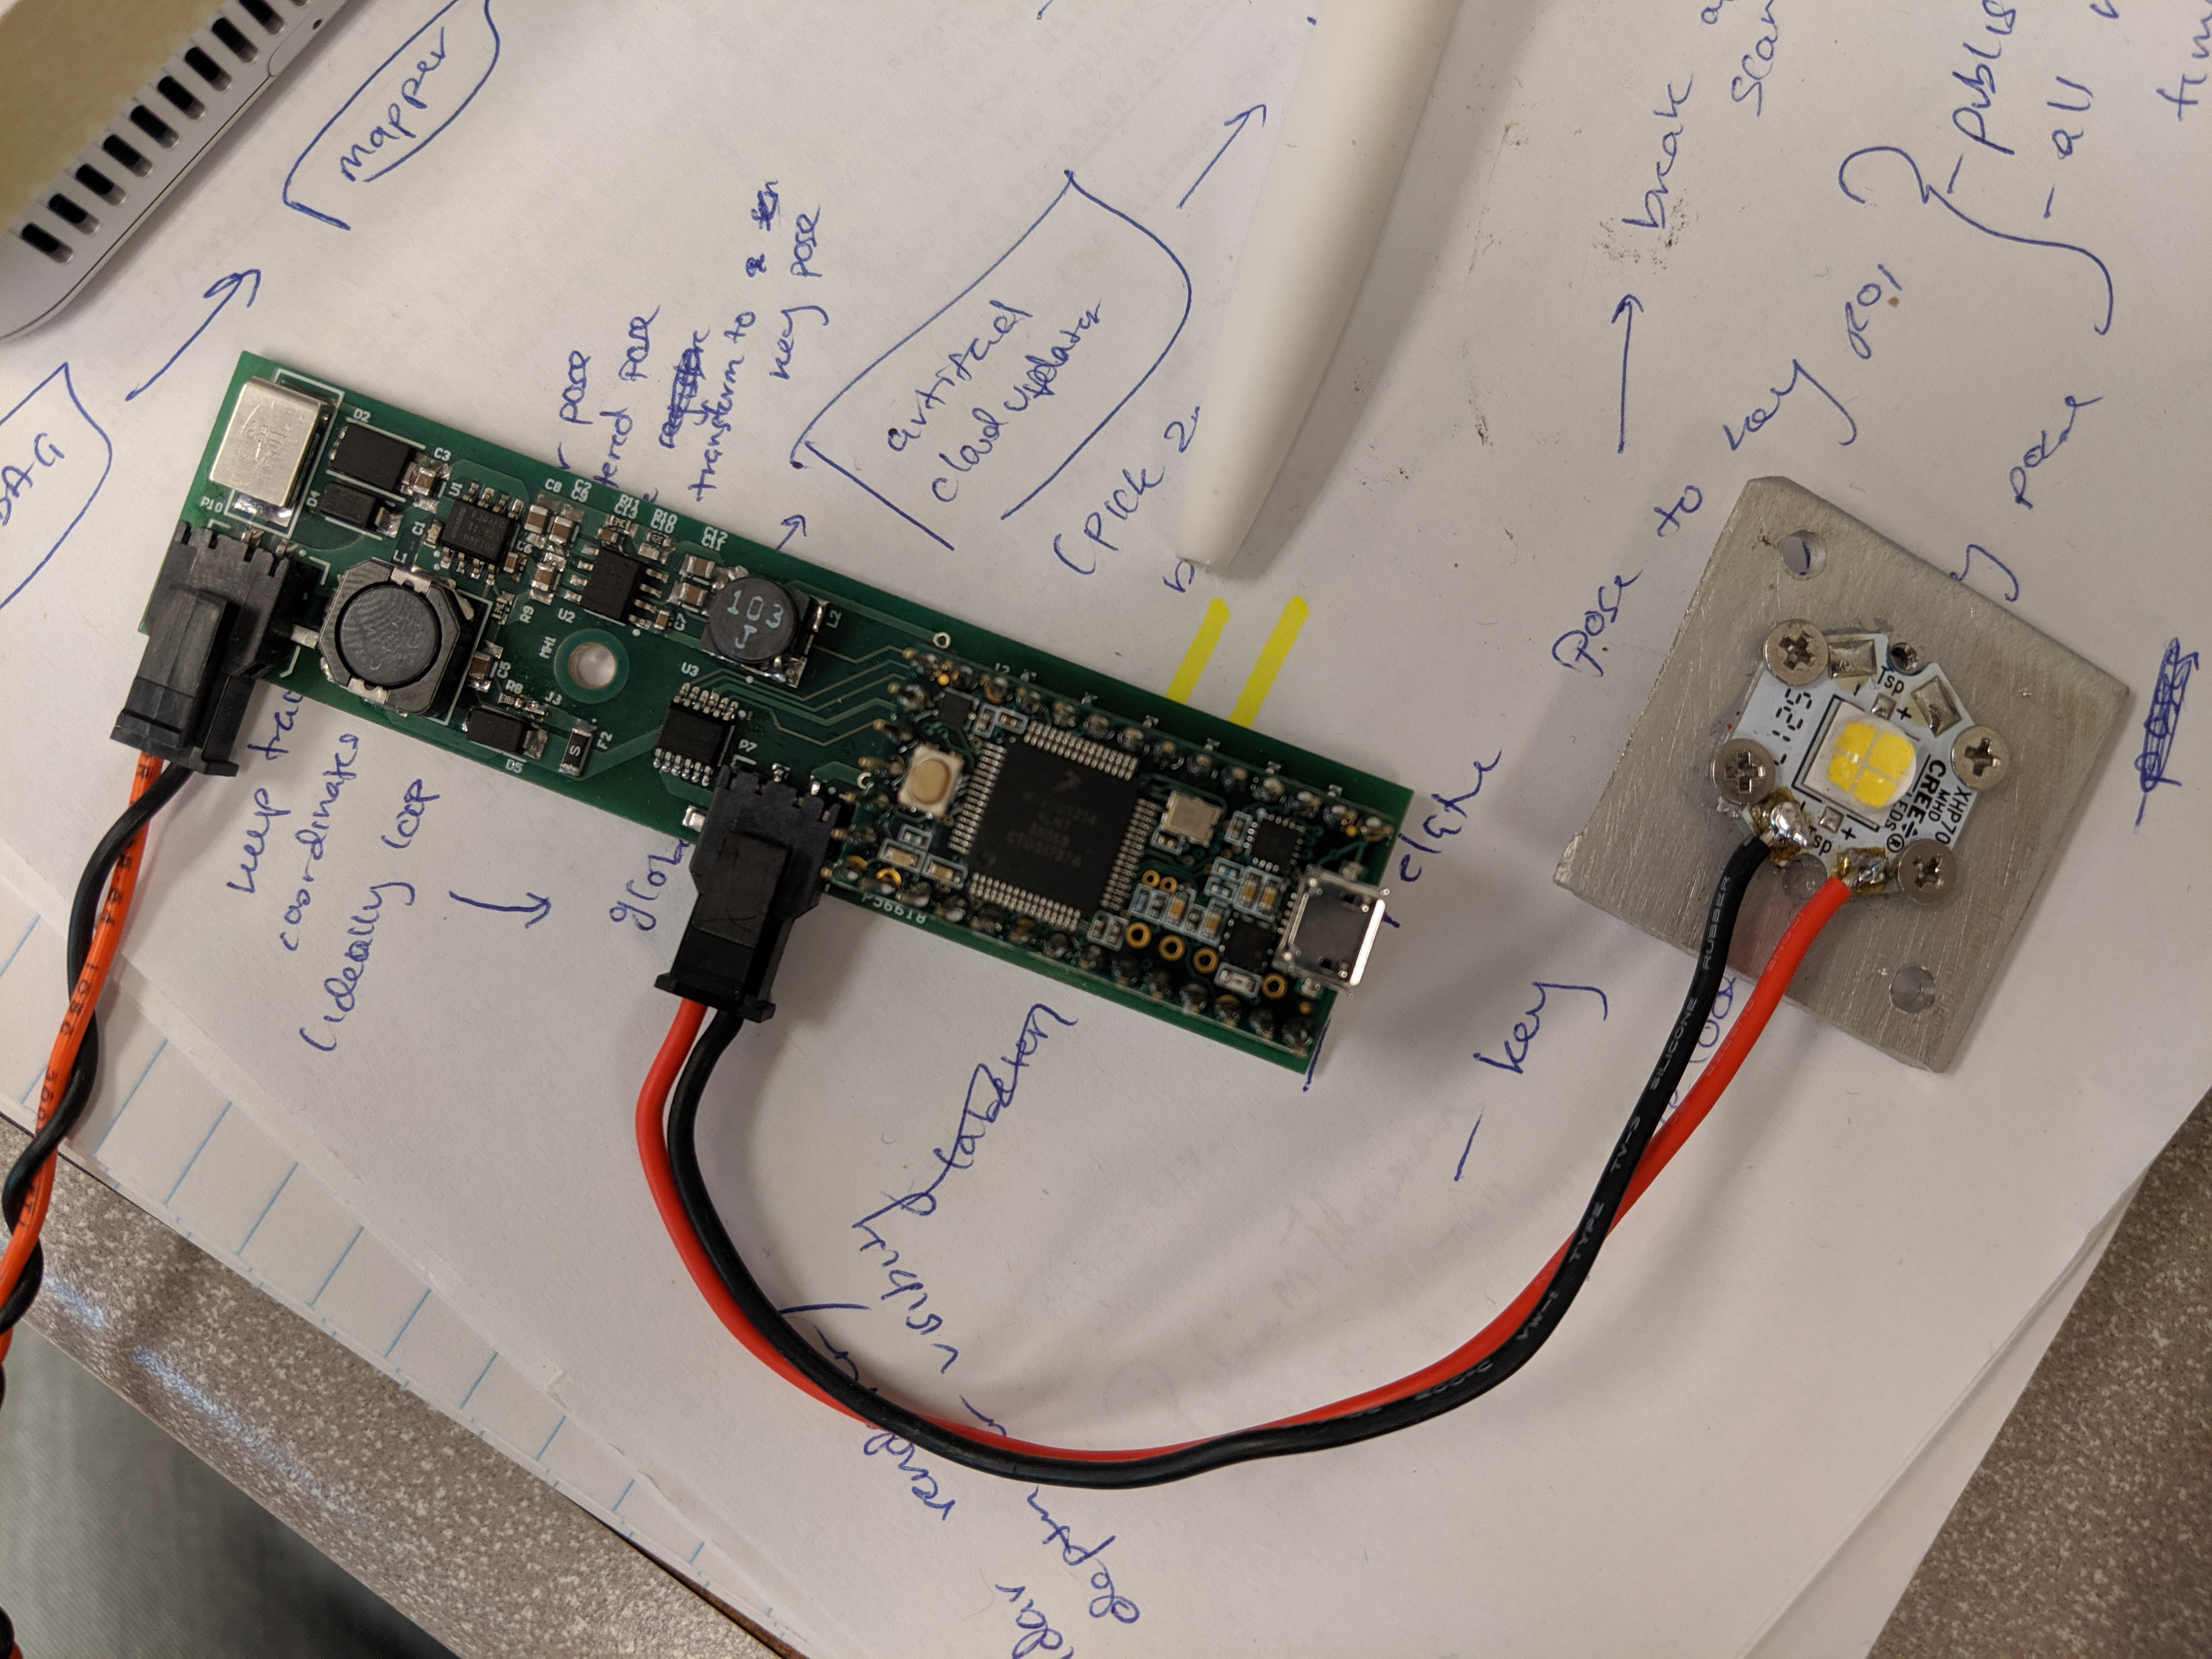
\includegraphics[width=.5\textwidth]{led_board.jpg}
	\caption[Custom PCB for LED control on Mk. 1]{This is the custom PCB developed for LED control on Mk. 1. The PCB is capable of brightness control over I2C and Serial for up to 2 LEDs, and can automatically turn them on with a trigger input from the RealSense camera modules. Unfortunately, the current requirements for 3 LEDs proved to be too great for the regulators on this PCB to handle, and there was not enough time left in the development cycle to fabricate new PCBs.}
	\label{led_board}
\end{figure}

\subsection{Miscellaneous Improvements}

A few small but useful improvements were made to the miscellaneous components used on Mk. 0 to improve reliability, robustness, or simplicity as a direct result of problems encountered when working on Mk. 0.

\subsubsection{Computer Power Buttons}

The computer power buttons used on Mk. 0 are relatively unreliable and do not indicate status of the computers. The power button for the NUC, for example, works very infrequently, and thus it has become standard (and inconvenient) operating procedure to use a small stick to poke the power button directly on the NUC. For Mk. 1, the power buttons have been replaced with rugged and illuminated metal power buttons which indicate computer power status. A blue LED is used for the NUC while a green LED is used for the Xavier.


\subsubsection{Ethernet Switch}

As mentioned previously, the original GigEthos switch in Mk. 0 failed randomly during field testing and was replaced with a commodity TP-Link gigabit Ethernet switch. For Mk. 1, the switch was further upgraded to a robust industrial grade gigabit network switch from Antaira with roughly the same footprint as the commodity one. The Antaira switch comes with screw terminals which make applying power from a regulator significantly easier than the commodity switch's barrel jack.

\subsubsection{Ethernet Connector}

The RJ-45 cable bulkhead used on Mk. 0 does not lock Ethernet cables very tightly, potentially allowing them to disconnect under strong vibration. Though this failure mode has not yet been experienced during field testing, it is likely to happen as the connector ages. For Mk. 1, an 8 pin connector from LEMO was used to create a custom connection for Ethernet. This solution has the added advantage of being significantly smaller than the RJ-45 bulkhead used on Mk. 0.

\subsubsection{LIDAR Cable Connector}

The cable for the LIDAR on Mk. 0 is passed through the case and wired directly into other components (e.g. power, network switch) without a connector. This makes servicing in the event of LIDAR failure (as in the case of the robot flipping over) difficult and time consuming. For Mk. 1, another locking connector from LEMO is used to allow easy LIDAR removal and replacement. Backup LIDARS have been prepared to allow replacement in a matter of minutes, rather than hours.

\subsubsection{Power Distribution Board}

Mk. 0 regulates 24V input down to 12V and 18V rails internally. Each regulator is a separate component from which wires are brought out to individual components. Though functional, this approach uses an abundance of wires which make any servicing inside Mk. 0 quite tedious. Mk. 1 instead uses a custom power distribution board with only a single 15V regulator, eliminating much of the wiring clutter and reducing component count. Use of the 15V regulator was now possible as the LED drivers could directly accept the input voltage to the payload and did not require a separate 12V rail.

\subsection{New Components}

Experience using Mk. 0, as well as the announcement of the actual Tunnel Circuit artifacts indicated that additional sensors and components could be useful for Mk. 1's functionality, as well as add some degree of future-proofing.

\subsubsection{Xavier WiFi Scanning}

WiFi scanning on Mk. 0 using the chip in the NUC takes an average of 3 seconds for a complete scan. At the ground robots' average speed of 2 m/s, this means the robots will typically move about 5 meters per scan. Assuming that the frequency of each individual scan cannot be improved due to library restrictions, the next best solution is to add a second chip capable of performing scanning. To this end, an Intel 8265 WiFi chip was added to the Xavier used in Mk. 1 to allow a second set of scans to run in parallel. Mk. 1 scans on both the NUC and Xavier simultaneously, and receives scan results at approximately 0.6 - 0.8 Hz.

\subsubsection{Microphone Array}

Though WiFi and Bluetooth scanning provide reliable presence detection for cell phones, accurate localization with the noisy signals produced from the scans is challenging. DARPA guarantees that the cell phones will be playing video with audio, meaning that audio can potentially be used as a secondary detection and localization mechanism. Mk. 1 includes a microphone array, the ReSpeaker Mic Array v2.0 from SeeedStudio, which provides 4 raw audio channels over USB. The audio streams can be fed into an algorithm such as ODAS \cite{grondin2019lightweight} to produce 3D direction of arrival estimates, which can be used for localization. This microphone array replaces the single microphone used in Mk. 0.

\subsubsection{Speaker}

The Mk. 0 payload has no way of communicating with or offering feedback to robot operators. Audio was selected as a viable feedback mechanism for Mk. 1 as it does not require line of sight as a screen would. The Large Surface Transducer from Adafruit was selected, along with an amplifier chip, to provide audio feedback. A transducer, pressed directly against the payload wall, is used instead of a traditional speaker in order to provide higher environmental robustness in the payload.

\section{Mk. 1 Assembly}

The assembly for Mk. 1 draws inspiration from Mk. 0, but differs in a few key areas to improve serviceability and reduce manufacturing time. Mk. 1 maintains the same multi-panel design as Mk. 0, but makes it possible to remove each of the 6 main panels from the cube, rather than gluing the 4 center panels together. This allows for a significant improvement in serviceability over Mk. 0. The computers have been moved from the sides of the payload to sheets in the center, with fans added to provide airflow and additional cooling. The fans are guarded by air filters and baffles to prevent dust and debris from entering the payload. The goal of flying Mk. 0 on a drone was entirely abandoned for Mk. 1, allowing thicker sheet metal to be used everywhere, improving the rigidity of the entire structure. Some pictures from the assembly of Mk. 1 are given in Figure \ref{mk_1_assembly}.

\begin{figure}
	\centering
	\begin{subfigure}{0.32\textwidth}
		\centering
		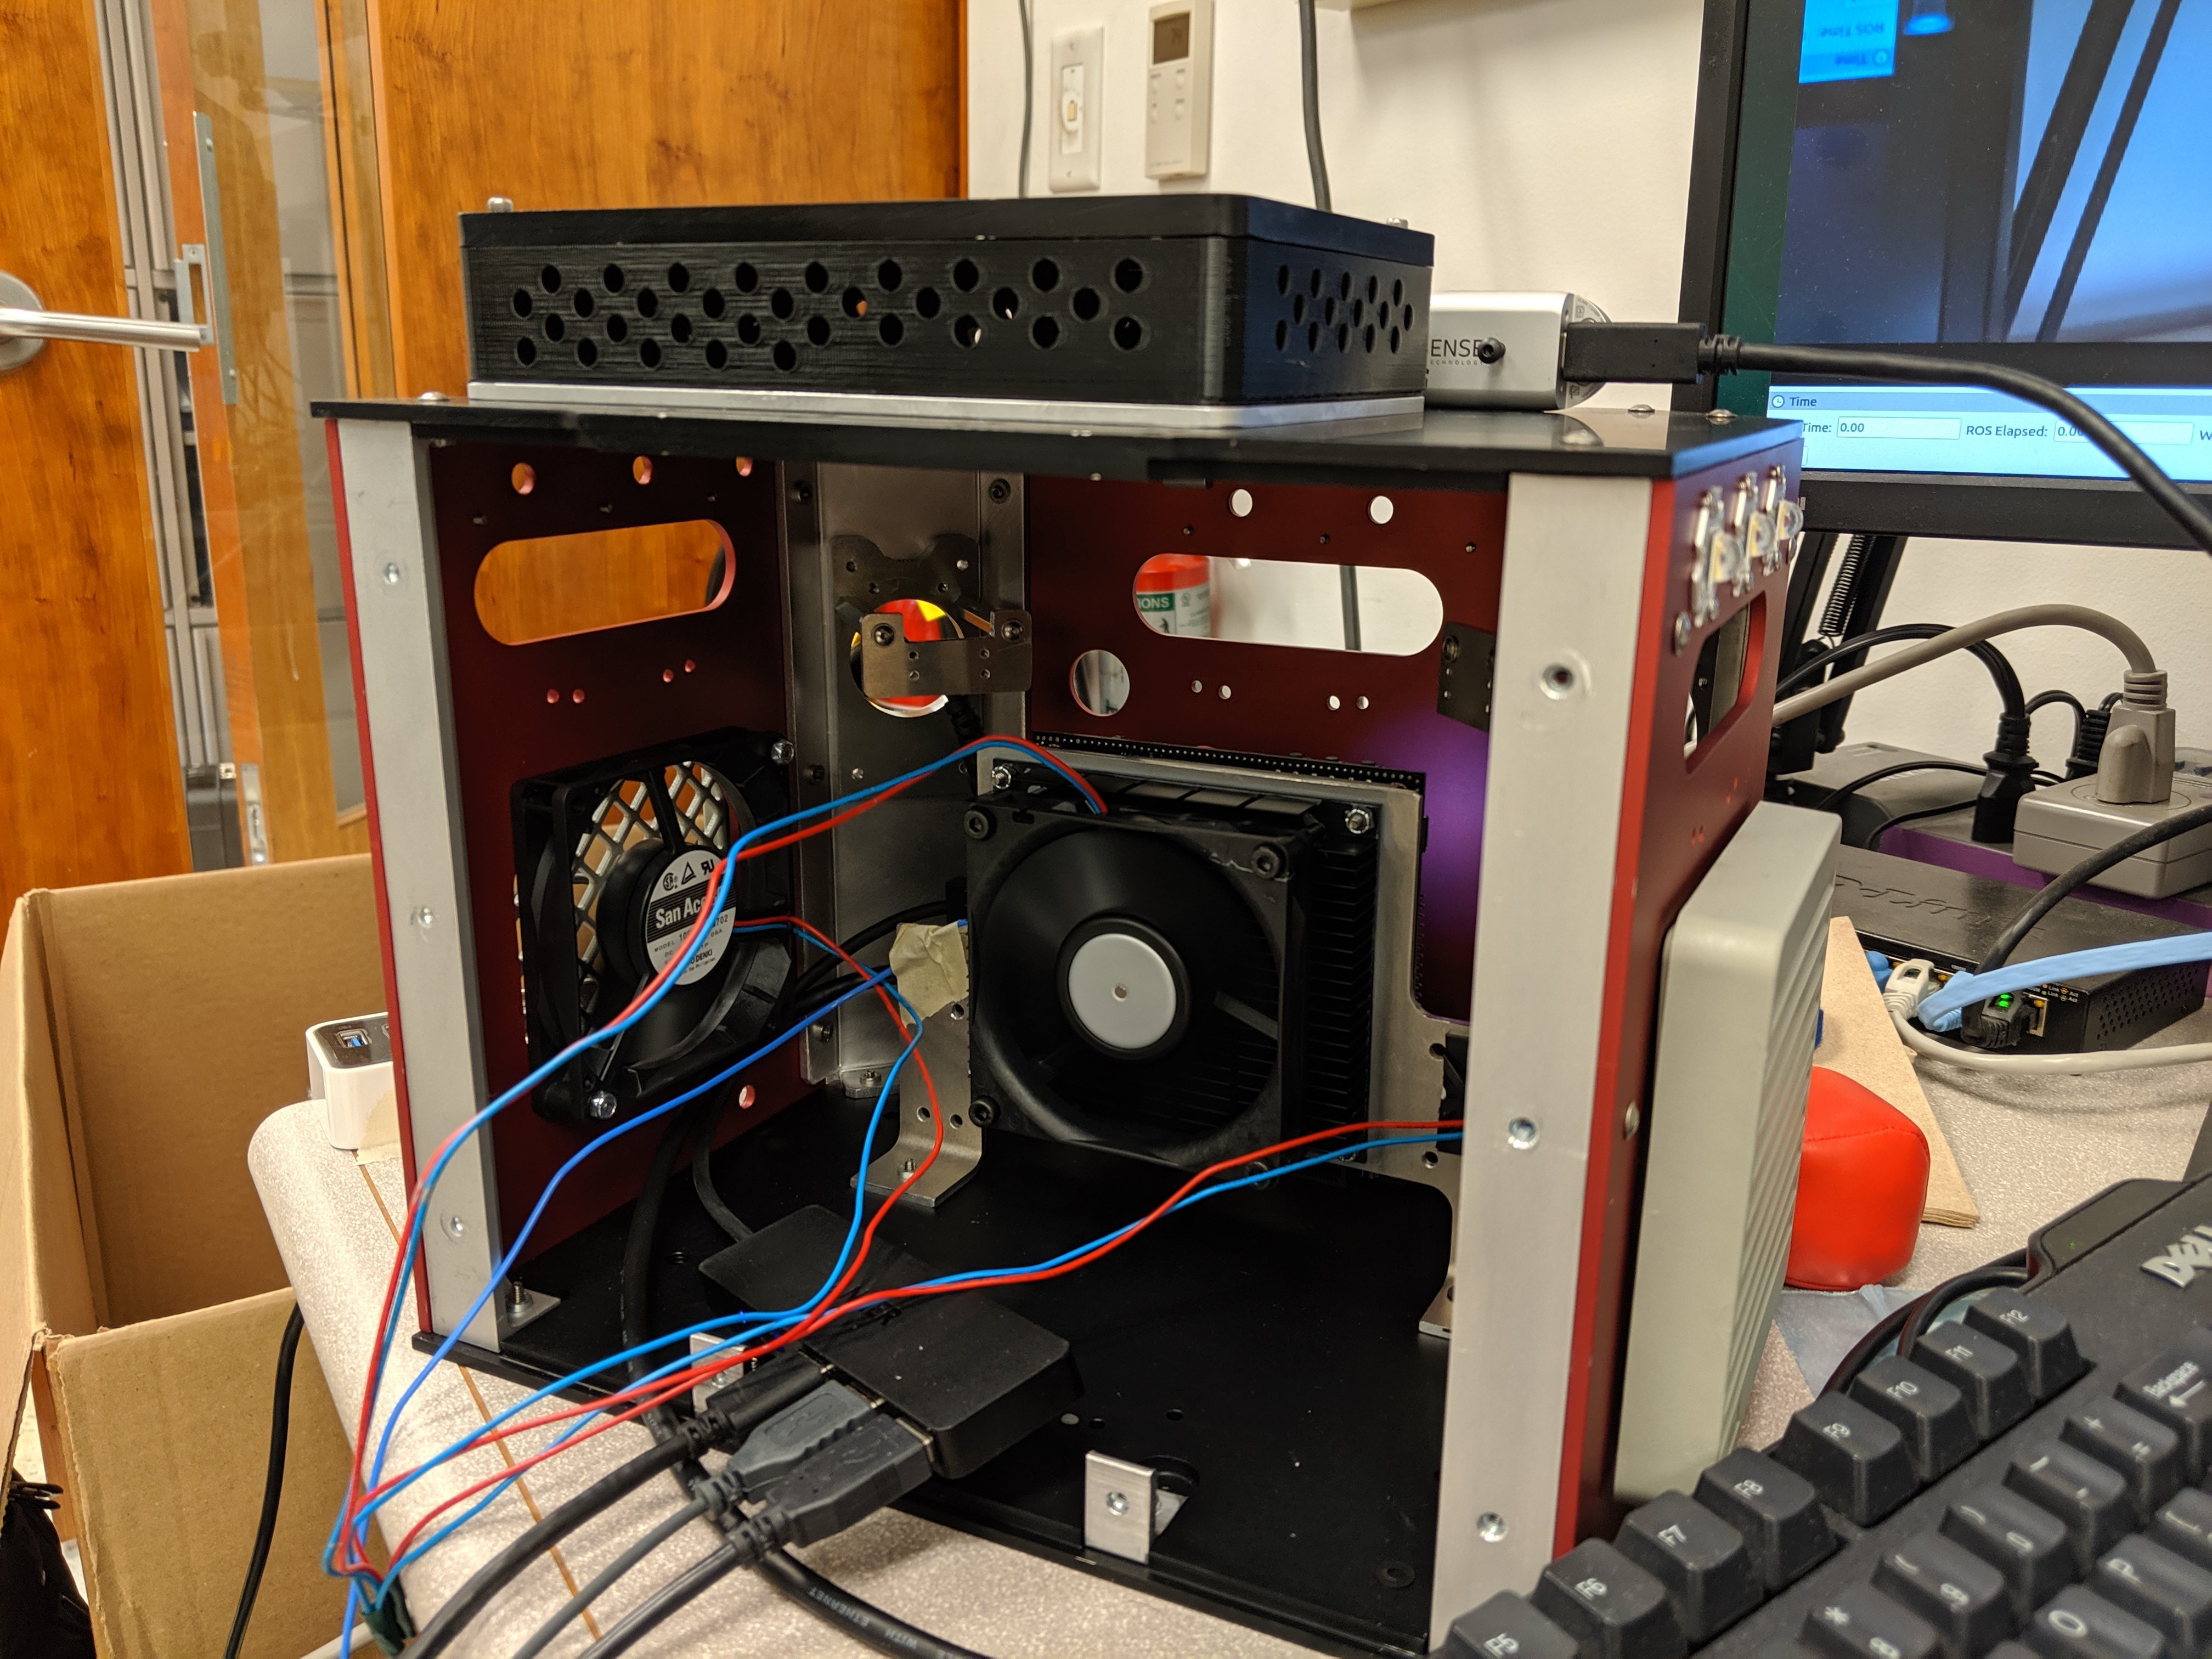
\includegraphics[width=\textwidth]{mk_1/interior.jpg}
		\caption{Xavier in interior panel}
		\label{mk_1_interior}
	\end{subfigure}
	\hfill
	\begin{subfigure}{0.32\textwidth}
		\centering
		\includegraphics[width=\textwidth]{mk_1/lit_up.jpg}
		\caption{Initial test of LEDs}
		\label{mk_1_lit_up}
	\end{subfigure}		
	\hfill
	\begin{subfigure}{0.32\textwidth}
		\centering
		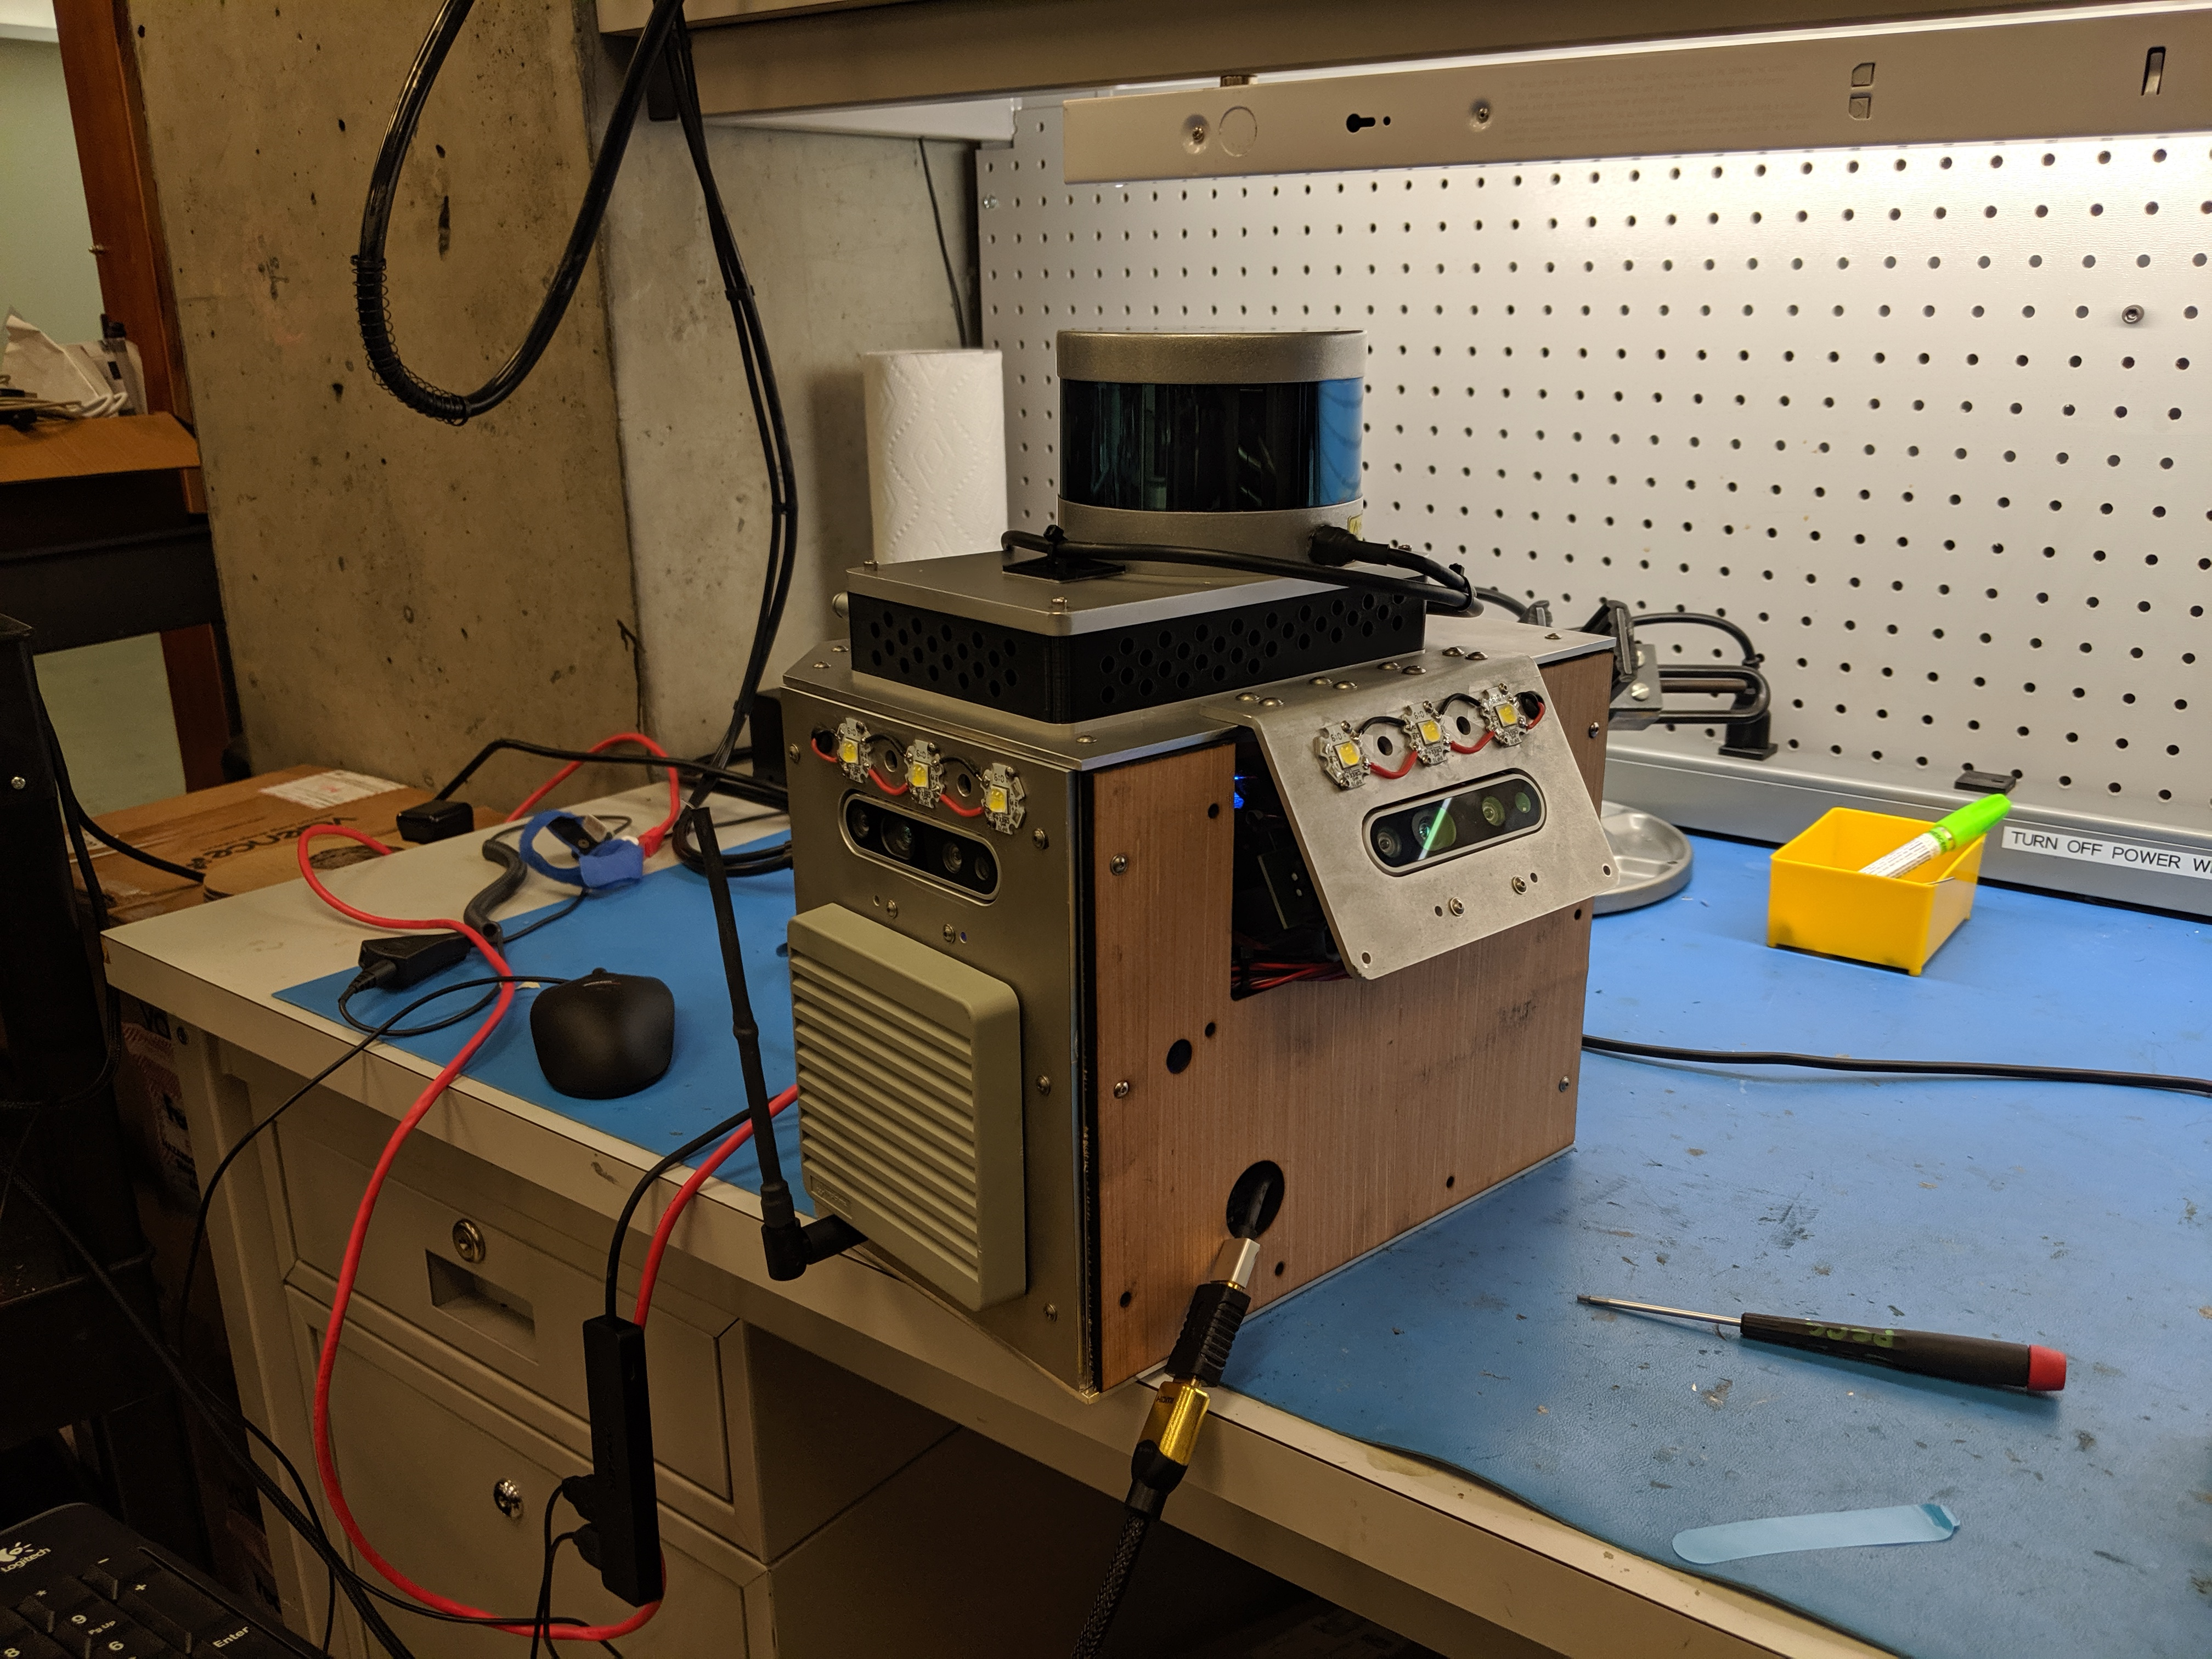
\includegraphics[width=\textwidth]{mk_1/wood_back.jpg}
		\caption{First button-up}
		\label{mk_1_wood_back}
	\end{subfigure}	
	\caption[Pictures from Mk. 1 assembly process]{The panel design used in Mk. 1 makes manufacturing and servicing significantly easier than Mk. 0. Careful consideration was also given to the assembly process, which is notably less painstaking than Mk. 0.}
	\label{mk_1_assembly}
\end{figure}

\section{Summary of Payloads} \label{Summary of Payloads}

This chapter describes the development of 3 distinct sensing and compute payloads. Each payload is capable of performing state estimation, path planning and navigation, and artifact detection and localization. A summary of the relevant components and capabilities of each payload is provided below. The Drone Payload is a simplified version of Mk. 0 meant for use on aerial platforms, while Mk. 1 is an incremental improvement on Mk. 0 using lessons learned over 6 months of development and use. See Figure \ref{payloads} for pictures of each payload.


\begin{description}
	\item[Drone Payload] \hfill
	\begin{itemize}
		\item \textbf{Compute}: Intel NUC8i7BEH
		\item \textbf{State Estimation}: Velodyne VLP-16 Puck LIDAR
		\item \textbf{State Estimation}: XSens IMU
		\item \textbf{RGB Camera}: RealSense D435 (front-facing)
		\item \textbf{Illumination}: 1x Opulent XHP70A 5000K LED
	\end{itemize}

	\item[Mk. 0 Payload] \hfill
	\begin{itemize}
		\item \textbf{Compute}: Intel NUC8i7BEH
		\item \textbf{Compute}: Nvidia Xavier with Developer Kit Carrier
		\item \textbf{State Estimation}: Velodyne VLP-16 Puck LIDAR
		\item \textbf{State Estimation}: XSens IMU
		\item \textbf{RGB Cameras}: 4x RealSense D435, up to 15 fps at 640 x 360 per camera
		\item \textbf{Thermal Camera}: FLIR Boson 320 w/ 92 degree HFOV, 320 x 256 at 8.5 fps
		\item \textbf{Audio Input}: 3.5mm audio input microphone
		\item \textbf{WiFi Scanning}: NUC builtin 9560 module
	\end{itemize}

	\item[Mk. 1 Payload] \hfill
	\begin{itemize}
		\item \textbf{Compute}: Intel NUC8i7BEH
		\item \textbf{Compute}: Nvidia Xavier with Developer Kit Carrier
		\item \textbf{State Estimation}: Velodyne VLP-16 Puck LIDAR
		\item \textbf{State Estimation}: XSens IMU
		\item \textbf{RGB Cameras}: 4x RealSense D435, up to 30 fps at 848 x 480 per camera
		\item \textbf{Thermal Camera}: 2x FLIR Boson 320 w/ 95 degree HFOV, 640 x 512 at 60 fps
		\item \textbf{Audio Input}: ReSpeaker Microphone Array V2.0
		\item \textbf{Audio Output}: Large Surface Transducer from Adafruit
		\item \textbf{WiFi Scanning}: NUC builtin 9560 module, Intel 8265 module in Xavier
	\end{itemize}
\end{description}

%problems to resolve for a future iteration:
%\begin{enumerate}
%	\item some light bleed / led glare on the realsense cameras. not sure why.
%	\item antennas need to be constantly checked since there's no way to force them to stay in their orientation
%	\item improved LED handling, yet again.
%	\item better speaker mounting? maybe use an actual speaker?
%	\item synchronization not addressed at all here
%	\item gas sensor
%\end{enumerate}